\documentclass[tikz]{article}

% Packages
\usepackage[utf8]{inputenc} % Core latex bundle 
\usepackage[a4paper, total={6in, 9in}]{geometry} % Customize document dimensions and formats
\usepackage{changepage} % Customize page layout in middle of document
\usepackage[table]{xcolor} % Add color to tables
\usepackage{standalone} % Add figures and tables from other files
\usepackage{import} % Import glossary
\usepackage{graphics} % General color and formats
\usepackage{url} % URL formatting
\usepackage{breakurl} % URL formatting
\usepackage{enumitem} % Format list spacing 
\usepackage[hang]{footmisc} % Footnote margins
\usepackage{hyperref} % References
\usepackage{mathtools} % Useful tools for mathematical typesetting and replaces amsmath
\usepackage{amssymb,bm} % Math symbols
\usepackage{svg} % SVG
\usepackage{tikz} % Making charts
\usepackage{array,boldline,multirow,float,booktabs} % Added to make tables
\usepackage{stackengine} % Customize row heights
\usepackage{hhline} % Add double lines to table
\usepackage{multicol} % Two column lists
\usepackage{nicematrix} % Put table lines after color
\usepackage{wrapfig} % Wrap figures in text
\usepackage{tocloft,titletoc} % TOC package
\usepackage{titlesec} % Section spacing
\usepackage{wasysym} % symbols
\usepackage{mathrsfs} % mathscr
\usepackage{setspace}

% Paper formatting
\newlength\LabelWidth
\setlength\parindent{0pt}
\setlength{\parskip}{1em}

% Section spacing
\titlespacing*{\section}
  {0pt}{0.6\baselineskip}{0.6\baselineskip} % Modify section spacing - first \baselineskip is spacing before, second is spacing after the section
\titlespacing*{\subsection}
  {0pt}{0.6\baselineskip}{0.6\baselineskip} % Modify subsection spacing 
\titlespacing*{\subsubsection}
  {0pt}{0.6\baselineskip}{0.6\baselineskip} % Modify subsubsection spacing

% String formats
\newcommand{\code}[1]{\texttt{#1}}
\newcommand{\term}[1]{\textsl{#1}}

% Paper margins
\def\changemargin#1#2{\list{}{\rightmargin#2\leftmargin#1}\item[]}
\let\endchangemargin=\endlist

% Table of contents
\renewcommand{\contentsname}{Table of Contents}
\renewcommand{\cfttoctitlefont}{\Large\bfseries} % TOC title size
\renewcommand{\cftsecleader}{\cftdotfill{\cftdotsep}} % Add dots in TOC to sections
\renewcommand{\cftsecpagefont}{} % Remove \bfseries from section titles' page in TOC

% Section
\renewcommand*{\cftsecnumwidth}{2em} % Increase space section from numbers on left

% Subsection
\cftsetindents{subsection}{1em}{3em} % space between numbers and toc subsections
\setlength{\cftsubsecindent}{2.5em} % subsection number spacing from left
\setlength{\cftbeforesubsecskip}{3pt} % Messes with subsection TOC length was 3pt

% Subsubsection
\cftsetindents{subsubsection}{1em}{4em} % space between numbers and toc subsubsections
\setlength{\cftsubsubsecindent}{5.5em} % subsubsection number spacing from leftindent
\setlength{\cftbeforesubsubsecskip}{3pt} % Messes with subsubsection TOC length was 3pt

% paragraph section
\setcounter{secnumdepth}{4}
\setcounter{tocdepth}{4}

\cftsetindents{paragraph}{1em}{5em} % space between numbers and toc paragraph
\setlength{\cftparaindent}{9.5em} % paragraph number spacing from leftindent
\setlength{\cftbeforeparaskip}{3pt} % Messes with paragraph TOC length was 3pt

% indent after paragraph section
\titleformat{\paragraph}
{\normalfont\normalsize\bfseries}{\theparagraph}{1em}{}
\titlespacing*{\paragraph}
{0pt}{3.25ex plus 1ex minus .2ex}{1.5ex plus .2ex}

% Abstract
% Make abstract justified
\makeatletter
\newcommand{\justified}{
  \rightskip\z@skip
  \leftskip\z@skip}
\makeatother

% Format and size abstract
\makeatletter
\renewenvironment{abstract}{
    \if@twocolumn
      \section*{\abstractname}
    \else 
      \begin{center}
        {\bfseries \large\abstractname\vspace{\z@}} % Bolds abstract name
      \end{center}
      \quotation
    \fi}
    {\if@twocolumn\else\endquotation\fi}
\makeatother

% Delimiters
\DeclarePairedDelimiter\floor{\lfloor}{\rfloor} % Define paired delimiter for floor function
\DeclarePairedDelimiter{\ceil}{\lceil}{\rceil} % Define paired delimiter for ceiling function

% Hyperlinks
\hypersetup{
    colorlinks=true,
    linkcolor=black,
    filecolor=blue,
    urlcolor=black,
}
\urlstyle{same}

% Footnotes
\newcommand{\fref}[1]{\footnote{\href{http://#1}{#1}}}
\setlength{\footnotemargin}{8mm} % Spacing between footnote number and body

% Include tables
\makeatletter
\newcommand{\includetable}[1]{%
  \@ifundefined{tablepath}{%
    \InputIfFileExists{#1}{}{}%
  }{%
    \InputIfFileExists{\tablepath/#1}{}{\InputIfFileExists{#1}{}{}}%
  }
}
\makeatother  

% Table formatting commands
\newcolumntype{Q}{ >{\centering\arraybackslash} m{2.4cm} } % (figures - col width)
\newcolumntype{S}{ >{\centering\arraybackslash} m{5.27cm} } % (figures - col width double)
\newcommand\xrowht[2][0]{\addstackgap[.5\dimexpr#2\relax]{\vphantom{#1}}} % Set row height for tables
\newcommand{\rowh}[1]{\xrowht{40pt}} % Command to set row height for cell with 3 rows
\newcommand{\rowm}[1]{\xrowht{26.667pt}} % Command to set row height for cell with 2 rows
\newcommand{\rows}[1]{\xrowht{13.333pt}} % Command to set row height for cell with 1 rows

\newcommand{\PintoCover}{\includesvg[scale=0.37]{./logos/black-pinto.svg}} % Logo on cover page
\newcommand{\PintoContract}{\includesvg[scale=0.032]{./logos/black-pinto.svg}} % Pinto contract used in paragraphs and formulas
\newcommand{\Pinto}{\includesvg[scale=0.032]{./logos/white-pinto.svg}} % Pinto used in paragraphs
\newcommand{\pinto}{\includesvg[scale=0.025]{./logos/white-pinto.svg}} % Pinto used in superscripts and subscripts
\newcommand{\nonpinto}{\includesvg[scale=0.022]{./logos/non-pinto.svg}} % Non-Pinto used in superscripts and subscripts

% List Key
\SetEnumitemKey{midsep}{topsep=0pt, itemsep=3pt} % Itemize key

% File paths
\newcommand{\tablepath}{figures} % Tables file path
\graphicspath{{figures/}} % Figures file path

%%%%%%%%%%%%%%%%%%%%%%%%%%%%%%%%%%%%%%   Begin Document   %%%%%%%%%%%%%%%%%%%%%%%%%%%%%%%%%%%%%%

\begin{document}
\pagenumbering{arabic} % Start page numbering style
\thispagestyle{empty} % Hide page numbering
\begin{titlepage}
    \begin{center}
        \vspace*{-0.1cm}
        \begin{changemargin}{-0.8cm}{-0.8cm}
            \centering % added to center title
            \textbf{\Large{Pinto: A Scalable Leviathan-Free Low-Volatility Money Protocol}}
        \end{changemargin}

        %%%%%%%%%%%%%%%%%%%%%%%%%%%%%%%%%%%%%%%%%%%% ICON %%%%%%%%%%%%%%%%%%%%%%%%%%%%%%%%%%%%%%%%%%%%
        
        \begin{center}
            \PintoCover
        \end{center}

        %%%%%%%%%%%%%%%%%%%%%%%%%%%%%%%%%%%%%%%%%%%% AUTHORS %%%%%%%%%%%%%%%%%%%%%%%%%%%%%%%%%%%%%%%%%%%%

        \begin{center}
            \begin{tabular}{>{\centering\arraybackslash}p{3.2cm} >{\centering\arraybackslash}p{3.2cm} >{\centering\arraybackslash}p{3.2cm} >{\centering\arraybackslash}p{3.2cm}}
                Brendan Sanderson & Ben Weintraub & Brian Nguyen & Austin Moninger \\
                \href{https://x.com/brendaann__}{\normalsize{x.com/brendaann\_\_}} & \href{https://x.com/bwein_}{\normalsize{x.com/bwein\_}} & \href{https://x.com/fr1j00}{\normalsize{x.com/fr1j00}} & \href{https://x.com/isthisaustin}{\normalsize{x.com/isthisaustin}}
            \end{tabular}
        \end{center}
        
        \vspace*{-0.52cm}

        \begin{center}
            \begin{tabular}{>{\centering\arraybackslash}p{4.6cm} >{\centering\arraybackslash}p{4.6cm} >{\centering\arraybackslash}p{4.6cm}}
                Drew Davis & Nikolaos Katsios & Ryan Ham \\
                \href{mailto:zsdrew@proton.me}{\normalsize{zsdrew@proton.me}} & \href{mailto:nkatsios@protonmail.com}{\normalsize{nkatsios@protonmail.com}} & \href{https://x.com/gkaehddls}{\normalsize{x.com/gkaehddls}}
            \end{tabular}
        \end{center}

        \vspace*{-0.52cm}

        \begin{center}
            \begin{tabular}{>{\centering\arraybackslash}p{4.6cm} >{\centering\arraybackslash}p{4.6cm} >{\centering\arraybackslash}p{4.6cm}}
                Calvin Ham & John Deere & Soil King \\
                 \href{mailto:calvinham@proton.me}{\normalsize{calvinham@proton.me}} & \href{mailto:johndeere8r420@protonmail.com}{\normalsize{johndeere8r420@protonmail.com}} & \href{mailto:soilking435@gmail.com}{\normalsize{soilking435@gmail.com}}
            \end{tabular}
        \end{center}

        \vspace*{-0.52cm}

        \begin{center}
            \begin{tabular}{>{\centering\arraybackslash}p{4.6cm} >{\centering\arraybackslash}p{4.6cm} >{\centering\arraybackslash}p{4.6cm}}
                Motasem Ahmed & Aaron Ash & Gabe Weintraub \\
                \href{https://x.com/itsmod323}{\normalsize{x.com/itsmod323}} & \href{mailto:aaron@aaronash.com}{\normalsize{aaron@aaronash.com}} & \href{mailto:gabeweintraub1@proton.me}{\normalsize{gabeweintraub1@proton.me}}
            \end{tabular}
        \end{center}

        %%%%%%%%%%%%%%%%%%%%%%%%%%%%%%%%%%%%%%%%%%%% WEBSITE AND DATES %%%%%%%%%%%%%%%%%%%%%%%%%%%%%%%%%%%%%%%%%%%%

        \normalsize{\href{https://pinto.money/}{pinto.money}}

        \footnotesize{Whitepaper Version:} {\normalsize{1.1.0}}

        \vspace{-0.25cm}
        \footnotesize{Published:} {\normalsize{April 2, 2025}}

        \vspace{-0.25cm}
        \footnotesize{Code Version:} \href{https://github.com/pinto-org/protocol/releases}{\normalsize{1.1.0}}\footnote{\href{https://github.com/pinto-org/protocol/releases}{github.com/pinto-org/protocol/releases}}

        \vspace{-0.25cm}
        \footnotesize{Deployed:} {\normalsize{March 12, 2025}}
        
        \vspace{0.1cm}

        \begin{adjustwidth}{1em}{1em} % Adjust margins equally
            \normalsize
            \term{“You broke the heads of Leviathan in pieces, and gave him to be meat to the people inhabiting the wilderness.”}
            
            \hspace{2.5em} - Psalm 74:14\fref{biblegateway.com/verse/en/Psalm\%2074:14}
        \end{adjustwidth}

        %%%%%%%%%%%%%%%%%%%%%%%%%%%%%%%%%%%%%%%%%%%% ABSTRACT %%%%%%%%%%%%%%%%%%%%%%%%%%%%%%%%%%%%%%%%%%%%

        \vspace*{-0.25cm}

        \begin{abstract}\setstretch{1.25}
            \justified{\normalsize{\noindent The ideal money is trustless and volatility free. Bitcoin is trustless, but has no native volatility minimization scheme. The tremendous success and adoption of Bitcoin as a store of value (SoV) has demonstrated the power of trustless technology and the primacy of trustlessness with respect to storing value. However, the widespread adoption of trusted stablecoins (\textit{e.g.}, USDT, USDC) as media of exchange (MoE) and units of account (UoA) on trustless computer networks has demonstrated the primacy of freedom from volatility with respect to exchanging and accounting for value. Because value is subjective, dynamic and relative, (1) money will never be entirely free from volatility, and (2) a money protocol optimizing for low volatility can not be trustless without the development of a trustless value index oracle. We propose a trust-minimized, low-volatility money protocol that issues a fungible token, Pinto, optimized to be a MoE and UoA. A bounty based timekeeping mechanism, non-custodial deposit and credit facilities, a variable supply and autonomously adjusting interest rates incentivize user behavior that minimizes the volatility of Pinto with respect to its value target over time, without ever forcing users to act or forcibly removing Pinto from their accounts. Future development of a trustless value index oracle can remove the only trust required by the protocol.}}
        \end{abstract}
   \end{center}
\end{titlepage}

\newpage

% TOC formatting
\thispagestyle{empty} % Hide TOC page numbering 
\addtocontents{toc}{\protect\thispagestyle{empty}} % Allow hiding both TOC page numbers

\cleardoublepage
\pagenumbering{gobble}
{\large\tableofcontents} % Compile TOC with large font
\cleardoublepage
\pagenumbering{arabic}

\newpage

\setcounter{page}{6} % Begin page numbering

%%%%%%%%%%%%%%%%%%%%%%%%%%%%%%%%%%%%%%   Introduction   %%%%%%%%%%%%%%%%%%%%%%%%%%%%%%%%%%%%%%

\section{Introduction}

The creation of Bitcoin began a technological revolution still in its infancy. Bitcoin proved the ability of open source software with endogenous incentives to create positive sum externalities (\textit{i.e.}, endogenous value), without requiring trust in any party or set of parties (\textit{i.e.}, a leviathan). Building an economy on such leviathan-free software that radically (1) empowers individuals with sovereignty and community, and (2) realigns incentives to encourage creating value instead of extracting it, is humanity's best bet to avoid being consumed by the ever more present technology-enabled Orwellian dystopia.

\vspace*{-0.1cm}

Money is the root of economy. It is no wonder, therefore, that Bitcoin (\textit{i.e.}, leviathan-free money) rang the bell to announce the revolution. However, money has historically fulfilled three unique but deeply complimentary roles in an economy: storing value, acting as a media through which to exchange value, and accounting for value. Bitcoin, incredible as it is, has only found product market fit as a SoV, not as a MoE or UoA. The volatility of the value of Bitcoin is the cause of the shortcoming. This is clearly demonstrated by the massive success of leviathan-dependent stablecoin protocols that issue tokens pegged to some exogenous unit of value, typically the US Dollar (USD) (\textit{i.e.}, the globally dominant MoE, UoA and, prior to the creation of Bitcoin, SoV) on trustless computer networks.

\vspace*{-0.1cm}

Trust is a least common denominator problem: a system requires as much trust as its component that requires the most trust. As of today, the reliance of users of, and protocols on, trustless computer networks (\textit{e.g.}, Ethereum, Solana) on leviathan-dependent MoE and UoA is so great that, in practice, the networks themselves lose their trustlessness: the authorities that control these protocols have so much power they are de facto the ultimate determinants of the state of the networks.\fref{haseebq.com/ethereum-is-now-unforkable-thanks-to-defi} Without a leviathan-free MoE and UoA, trustless systems will struggle to remain free from leviathans.

\vspace*{-0.1cm}

Credit is the ideal tool to minimize volatility because it (1) enables using future value in the present, (2) is infinitely scalable, and (3) does not require a leviathan. During periods of excess supply (\textit{i.e.}, insufficient demand), Pinto uses credit to call forward future demand to the present. In practice, the protocol borrows Pinto from the market and then burns the borrowed excess Pinto to decrease the supply, thereby reducing downside volatility. During periods of excess demand (\textit{i.e.}, insufficient supply) the protocol mints new Pinto and pays back creditors with interest, thereby reducing upside volatility. The more debt Pinto repays with interest, the more (1) creditworthy it is perceived, (2) it can borrow at lower interest rates, and (3) it can sustainably reduce future downside volatility. 

\vspace*{-0.1cm}

Pinto consists of four interconnected components: (1) a bounty based timekeeping and execution facility, (2) a liquid deposit facility, (3) a first in, first out (FIFO) credit facility, and (4) a suite of tools that reduce the friction of interacting with Pinto and other Base-native protocols. Protocol-native incentives coordinate the components to create low-volatility money with competitive carrying costs and deep liquidity in a permissionless and (almost) leviathan-free fashion.

\vspace*{-0.1cm}

Pinto is designed from economic first principles to create low-volatility money. The following principles inspire Pinto:

\vspace*{-0.3cm}

\begin{itemize}[itemsep=0.03cm]
    \item Incentive structures determine behaviors;
    \item Low concentration of ownership;
    \item Strong credit;
    \item Deep liquidity;
    \item The marginal rate of substitution;
    \item Low friction; and
    \item Equilibrium.
\end{itemize}

%%%%%%%%%%%%%%%%%%%%%%%%%%%%%%%%%%%%%%   Previous Work   %%%%%%%%%%%%%%%%%%%%%%%%%%%%%%%%%%%%%%

\section{Previous Work}

Pinto is the culmination of previous development, evolution and experimentation within the DeFi ecosystem. 

Pinto requires a robust, trustless computer network that supports composability and both fungible and semi-fungible token standards (\term{e.g.}, Ethereum and Base) with a network-native automated market maker (AMM) decentralized exchange with a manipulation-resistant oracle (\term{e.g.}, Pinto Exchange\fref{pinto.exchange}). 

Pinto was inspired by Beanstalk\fref{bean.money}. The performance of Beanstalk and other algorithmic stablecoin implementations provided invaluable information that influenced the design of Pinto. A significant portion of the Pinto codebase was forked from the Beanstalk codebase.


%%%%%%%%%%%%%%%%%%%%%%%%%%%%%%%%%%%%%%%% Farm %%%%%%%%%%%%%%%%%%%%%%%%%%%%%%%%%%%%%%%%

\section{Farm}

Well designed decentralized protocols create utility for end users without requiring, but never preventing, participation in protocol maintenance. Protocol-native incentives encourage performance of work to create utility for end users. Low barriers to and variety in work enable a diverse set of participants. A diverse set of well incentivized workers can create censorship resistant utility. 

Pinto peg maintenance takes place on the \term{Farm}. Anyone can join the \term{Farm} to profit from participation in protocol maintenance. The \term{Farm} has four primary components: the \term{Sun}, \term{Silo}, \term{Field} and \term{Toolshed}. Protocol-native financial incentives coordinate the components to regularly cross the price of \Pinto1 over its value target without collateral.

The \term{Sun} offers payment for participating in timekeeping and code execution. Time on the \term{Farm} is kept in \term{Seasons}. Anyone can earn Pinto for successfully calling the \code{gm} function to begin the next \term{Season} at the top of each hour.

The \term{Silo} offers passive yield opportunities to owners of \Pinto\ and other assets ($\lambda$) on the \term{Deposit Whitelist} ($\Lambda$) (\textit{i.e.}, $\Pinto \subset \lambda \in \Lambda$) for contributing to peg maintenance. Anyone can become a \term{Stalkholder} by \term{Depositing} $\lambda$ into the \term{Silo} and earning \term{Stalk}. \term{Stalkholders} are rewarded Pinto when the Pinto supply increases on a pro rata basis. Active contributions to peg maintenance within the \term{Silo} can earn additional \term{Stalk}.

The \term{Field} offers yield opportunities to creditors for supporting peg maintenance. Anyone can become a \term{Sower} by lending Pinto that are not in the \term{Silo} to the protocol. \term{Sowers} are repaid with interest when the Pinto supply increases on a first in, first out (FIFO) basis. 

The \term{Toolshed} offers a suite of tools that decrease friction to using the protocol and participating in peg maintenance.

%%%%%%%%%%%%%%%%%%%%%%%%%%%%%%%%%%%%%%   Sun   %%%%%%%%%%%%%%%%%%%%%%%%%%%%%%%%%%%%%%

\section{Sun}

The Pinto peg maintenance mechanism requires a protocol-native timekeeping mechanism and regular code execution on the Base network. The \term{Sun} creates a cost-efficient protocol-native timekeeping mechanism and incentivizes cost-efficient code execution on Base at regular intervals. In general, Pinto uses Base block timestamps ($E$), such that $E \in \mathbb{Z}^{+}$.

\newpage

We define a \term{Season} ($t$), such that $t \in \mathbb{Z}^{+}$, as an approximately 3,600 second (1 hour) interval. The first \term{Season} begins when a successful transaction on the Base network that includes a \code{gm} function call is committed. When Pinto accepts the \code{gm} function call, the necessary code is executed.

Pinto only accepts one \code{gm} function call per \term{Season}. Pinto accepts the first \code{gm} function call provided that the timestamp in the Base block containing it is sufficiently distant from the timestamp in the Base block containing the Pinto deployment ($E_{1}$).

The minimum timestamp Pinto accepts a \code{gm} function call for a given $t$ ($E_{t}^{\text{min}}$), $\forall\ E_{t}^{\text{min}}$ such that $1 < t$, and $E_{1}$ is:

    $$
        E_{t}^{\text{min}} = 
            3600{\left
                ({\left\lfloor\frac{E_{1}}{3600}\right\rfloor} + t\right)}
    $$

The cost to execute the \code{gm} function changes depending on the traffic on the Base network and the state of Pinto. Pinto covers the transaction cost by rewarding the sender of an accepted \code{gm} function call with newly minted Pinto. 

To encourage regular \code{gm} function calls even during periods of congestion on the Base network while minimizing cost, the Pinto reward for successfully calling the \code{gm} function for $t$ ($a_{t}$), starts at $\sun$, such that $a_{t},\ \sun \in \{j \times 10^{-6} \mid j \in \mathbb{Z}^{+} \}$, and compounds 2.01\% every additional 2 seconds that elapse past $E_{t}^{\text{min}}$ for 300 seconds.

Therefore, we define $a_{t}$ for a given timestamp of the current block ($E_{\Xi}$) and $E_{t}^{\text{min}}$ as:

    $$ 
        a_{t} = \sun \times 1.0201^{\text{min}(
                    2 \times \left \lceil \frac{E_{\Xi} - E_{t}^{\text{min}}}{2} \right \rceil,\ 
                    300)}
    $$

To minimize the cost of calculating $a_{t}$, the \term{Sun} uses a binomial estimation with a margin of error of less than 0.05\% of $a_{t}$. Thus, Pinto creates a cost-efficient protocol-native timekeeping mechanism and ensures cost-efficient code execution on the Base network at regular intervals.

%%%%%%%%%%%%%%%%%%%%%%%%%%%%%%%%%%%%%%   Silo   %%%%%%%%%%%%%%%%%%%%%%%%%%%%%%%%%%%%%%

\vspace*{-1mm}
\section{Silo}
\vspace*{-1mm}

The \term{Silo} is the protocol-native \term{Deposit} facility.

The \term{Silo} uses the \term{Stalk System} to create protocol-native financial incentives that contribute to security and peg maintenance. The \term{Silo} uses the \term{Seed Gauge System} to create protocol-native financial incentives that contribute to peg maintenance. Anyone can become a \term{Stalkholder} by \term{Depositing} assets on the \term{Deposit Whitelist} into the \term{Silo} to earn \term{Stalk} and \term{Seeds}.

%%%%%%%%%%% Deposits, Withdrawals, Transfers and Conversions %%%%%%%%%%%

\vspace*{-1.2mm}
\subsection{Deposits, Withdrawals, Conversions and Transfers}
\vspace*{-1.2mm}

$\lambda$ can be \term{Deposited} into, \term{Withdrawn} from and \term{Transferred} within the \term{Silo} at any time. $\lambda$ can be \term{Converted} within the \term{Silo} under permitted conditions. 

The protocol rewards \term{Stalk} to \term{Depositors} upon the completion of a \term{Germination} period. The protocol rewards \term{Seeds} to \term{Depositors} immediately upon \term{Depositing} $\lambda$ into the \term{Silo}. \term{Deposits} implement the ERC-1155 Standard.\fref{ethereum.org/en/developers/docs/standards/tokens/erc-1155}

Upon a \term{Deposited} asset's \term{Withdrawal} from the \term{Silo}, the \term{Deposit} token is burned in addition to the number of \term{Stalk} and \term{Seeds} rewarded to it. 

\vspace*{1.2mm}

\term{Conversions} of \term{Deposited} $\lambda$ to \term{Deposited} $\lambda'$ are permissioned by a \term{Conversion Whitelist}. Upon an asset's \term{Conversion} within the \term{Silo}, \term{Stalk} and \term{Seeds} may be rewarded or burned depending on the details of the \term{Conversion}.

\vspace*{1.2mm}

The number of \term{Stalk} and \term{Seeds} rewarded to a \term{Deposit} are included in its \term{Transfer} to another address.

%%%%%%%%%%%%%%%%%%%%%%% Deposit Whitelist %%%%%%%%%%%%%%%%%%%%%%%

\vspace*{1.2mm}
\subsubsection{Deposit Whitelist}
\vspace*{1.2mm}

Any ERC-20 Standard token can be added to and removed from $\Lambda$ via the \term{Pinto Contract Multisig} (\term{PCM}) (see Appendix). \Pinto\ is always on the \term{Deposit Whitelist}.

\vspace*{1.2mm}

In order for a given $\lambda$ to be added to $\Lambda$, the protocol requires 
(1) its token address, 
(2) a function to calculate the flash-loan-resistant Pinto-Denominated-Value (PDV) of a given number of \term{Deposited} $\lambda$, ($f^{L^{\lambda}}(z^{\lambda})$), such that $f^{L^{\lambda}}\colon \{j \times 10^{-\lambda} \mid j \in \mathbb{Z}^{+} \} \rightarrow \{j \times 10^{-6} \mid j \in \mathbb{Z}^{+} \}$, where $z^{\lambda}$ is the number of $\lambda$ \term{Deposited}, 
(3) the number of \term{Stalk} per PDV of $\lambda$ \term{Deposited} ($k^{\lambda}$), such that $k^{\lambda} \in \{j \times 10^{-16} \mid j \in \mathbb{Z}^{+} \}$, 
(4) the initial number of \term{Seeds} per PDV of $\lambda$ \term{Deposited} ($c_{\circ}^{\lambda}$),
(5) the initial \term{LP Seed Gauge Points} of $\lambda$ ($\mathscr{L}_{\circ}^{\lambda}$), such that $\mathscr{L}_{\circ}^{\lambda} \in \{j \times 10^{-18} \mid j \in \mathbb{Z}^{+} \}$,
(6) a function to calculate the \term{LP Seed Gauge Points} of $\lambda$ ($f^{\mathscr{L}^{\lambda}}$), 
(7) a function to calculate the USD price of the non-Pinto asset in $\lambda$ ($f^{\$^{\lambda}}$), such that $f^{\$^{\lambda}} \colon \mathbb{U} \rightarrow \{j \times 10^{-6} \mid j \in \mathbb{Z}^{+} \}$,
(8) a function to calculate the \term{Liquidity Weight} of $\lambda$ ($f^{\mathscr{W}^{\lambda}}$), such that $f^{\mathscr{L}^{\lambda}},\ f^{\mathscr{W}^{\lambda}} \colon \mathbb{U} \rightarrow \{j \times 10^{-18} \mid j \in \mathbb{Z}^{+} \}$, and
(9) the optimal percent of \term{Deposited} LP PDV of $\lambda$ ($\mathscr{B}^{\lambda^{*}}$), such that $z^{\lambda},\ c_{\circ}^{\lambda},\ \mathscr{B}^{\lambda^{*}} \in \{j \times 10^{-6} \mid j \in \mathbb{Z}^{+} \}$.

%%%%%%%%%%%%%%%%%%%%%%% Earned Pinto %%%%%%%%%%%%%%%%%%%%%%%

\vspace*{1.2mm}
\subsubsection{Earned \Pinto}
\vspace*{1.2mm}

Pinto minted to the \term{Silo} are automatically \term{Deposited} into the \term{Silo} and distributed to \term{Stalkholders} as \term{Earned} \Pinto\ ($\eta^{\pinto}$), such that $\eta^{\pinto} \in \{j \times 10^{-6} \mid j \in \mathbb{N} \}$.

\vspace*{1.2mm}

\term{Earned} \Pinto\ are rewarded \term{Stalk} upon \term{Deposit}, but (1) are not rewarded \term{Seeds}, (2) cannot be \term{Converted} and (3) cannot be \term{Transferred} until the \term{Stalkholder} calls the \code{plant} function. Upon calling the \code{plant} function, (1)  the \term{Earned} \Pinto\ become \Pinto\ and (2) the \term{Seeds} associated with the \term{Earned} \Pinto\ are \term{Planted} to start \term{Growing} \term{Stalk}. 

%%%%%%%%%%%%%%%%%%%%%%% Germination %%%%%%%%%%%%%%%%%%%%%%%

\vspace*{1.2mm}
\subsubsection{Germination}
\vspace*{1.2mm}

Every $\lambda$ \term{Deposit} except \term{Earned} \Pinto\ are subject to a \term{Germination} period during which \term{Deposits} (1) cannot be \term{Converted}, (2) are not eligible for \Pinto\ mints and (3) are not included in \term{Seed Gauge System} PDV calculations. 

\vspace*{1.2mm}

\term{Germination} ends upon the completion of a full \term{Season} after \term{Deposit}.

\newpage

%%%%%%%%%%%%%%% Silo Figure %%%%%%%%%%%%%%%

\begin{figure}[h!]
    \centering
    \includegraphics[scale=.12]{figures/Silo.png}
    \vspace*{-5mm}
    \caption{Silo}
    \label{Silo}
\end{figure}

%%%%%%%%%%%%%%%%%%%%%%% Conversion Whitelist %%%%%%%%%%%%%%%%%%%%%%%

\subsubsection{Conversion Whitelist}

\term{Conversions} can be added to and removed from the \term{Conversion Whitelist} via the \term{PCM}.

In order for a given \term{Conversion} to be added to the \term{Conversion Whitelist}, the protocol requires 
(1) the from token address, 
(2) the to token address, 
(3) a list of conditions under which the \term{Conversion} is permitted and 
(4) a function to determine the number of $\lambda'$ received for \term{Converting} a given number of $\lambda$ ($f^{\lambda \rightarrow \lambda'}(z^{\lambda})$), such that $f^{\lambda \rightarrow \lambda'}\colon \{j \times 10^{-\lambda} \mid j \in \mathbb{Z}^{+} \} \rightarrow \{j \times 10^{-\lambda'} \mid j \in \mathbb{Z}^{+} \}$, where $z^{\lambda}$ is the number of $\lambda$ \term{Converted} or 
(5) a function to determine the number of \term{Mown Stalk} rewarded or burned for \term{Converting} a given number of $\lambda$ to $\lambda'$ ($f^{\lambda \rightarrow \lambda'}(z^{\lambda} \rightarrow z^{\lambda'})$), such that $f^{\lambda \rightarrow \lambda'}\colon \{j \times 10^{-\lambda} \rightarrow j' \times 10^{-\lambda'} \mid j,\ j' \in \mathbb{Z}^{+} \} \rightarrow \{j \times 10^{-16} \mid j \in \mathbb{Z}^{+} \}$, where $z^{\lambda}$ is the number of $\lambda$ \term{Converted} and where $z^{\lambda'}$ is the number of $\lambda$ output by the \term{Conversion}. 

%%%%%%%%%%%%%%%%%%%%%%% Stalk System %%%%%%%%%%%%%%%%%%%%%%%

\vspace*{-1.35mm}
\subsection{Stalk System}
\vspace*{-1.35mm}

The \term{Stalk System} decentralizes ownership of \Pinto\ over time and creates protocol-native financial incentives to (1) \term{Deposit} assets into the \term{Silo}, (2) leave assets \term{Deposited} in the \term{Silo} and (3) align \term{Depositors'} interests with the health of the protocol.

\term{Stalk} are not liquid. Every \term{Season}, $\frac{1}{10000}$ additional \term{Stalk} \term{Grows} from each \term{Seed}. \term{Grown Stalk} become \term{Stalk} when \term{Mown}. Upon a \term{Deposited} asset's \term{Withdrawal} from the \term{Silo}, the number of \term{Stalk} and \term{Grown Stalk} rewarded to it must be burned.

\term{Stalkholders} are entitled to a portion of Pinto mints. The distribution of Pinto paid to a \term{Stalkholder} are proportional to their \term{Stalk} holdings relative to total outstanding \term{Stalk}. \term{Stalk} holdings become less concentrated over time. Active contributions to peg maintenance within the \term{Silo} can earn additional \term{Stalk} via \term{Conversions}.
 
\term{Grown Stalk} from $\lambda$ \term{Deposits} are automatically \term{Mown} each time a \term{Stalkholder} interacts with $\lambda$ in the Silo (\textit{i.e.}, \term{Deposit}, \term{Withdraw}, \term{Convert}, \term{Transfer} and \term{Plant}), or anytime a \code{mow} function is called with $\lambda$ and their address.

%%%%%%%%%%%%%%%%%%%%%%% Seed Gauge System %%%%%%%%%%%%%%%%%%%%%%%

\vspace*{-1.35mm}
\subsection{Seed Gauge System}
\vspace*{-1.35mm}

The \term{Seed Gauge System} decentralizes ownership of \Pinto\ over time and creates protocol-native financial incentives to (1) \term{Deposit} assets into the \term{Silo}, (2) leave assets \term{Deposited} in the \term{Silo} and (3) align \term{Depositors'} interests with the health of the protocol.

\term{Seeds} are not liquid. At the beginning of each \term{Season}, the total number of \term{Seeds} is calculated such that a new \term{Deposit} with an average number of \term{Seeds} per PDV, averaged across all \term{Deposits} in the \term{Silo} that are not \term{Germinating}, will catch up to the average \term{Mown Stalk} per PDV across all \term{Deposits} in the \term{Silo} at the beginning of $t$ in $\mathscr{T}$ \term{Seasons}, such that $\mathscr{T}\in \mathbb{Z}^{+}$.

The \term{Crop Ratio} during $t$ ($\mathscr{C}_{t}$), such that $\mathscr{C}_{t} \in \{j \times 10^{-18} \mid j \in \mathbb{Z}^{+} \}$, determines the ratio between (1) the \term{Seeds} per \Pinto\ \term{Deposited} in the \term{Silo} that are not \term{Germinating} at the beginning of $t$ ($\mathbf{L}_{t}^{\pinto}$) (\textit{i.e.}, $\frac{c_{t}^{\pinto}}{\mathbf{L}_{t}^{\pinto}}$) and (2) the \term{Seeds} per PDV of the $\lambda$ with the highest \term{LP Seed Gauge Points} per PDV of $\lambda$ \term{Deposited} in the \term{Silo} that are not \term{Germinating} at the beginning of $t$ ($\mathbf{L}_{t}^{\lambda^{\text{max}}}$) (\textit{i.e.}, $\frac{c_{t}^{\lambda}}{\mathbf{L}_{t}^{\lambda^{\text{max}}}}$), such that $\mathbf{L}_{t}^{\pinto},\ \mathbf{L}_{t}^{\lambda^{\text{max}}} \in \{j \times 10^{-6} \mid j \in \mathbb{Z}^{+} \}$.

The distribution of \term{Seeds} across $\lambda$ during $t$ is a function of (1) the \term{Crop Ratio} and (2) the distribution of \term{LP Seed Gauge Points}.

%%%%%%%%%%%%%%%%%%%%%%% Calculating Stalk %%%%%%%%%%%%%%%%%%%%%%%

\vspace*{-1mm}
\subsection{Calculating Stalk}
\vspace*{-1mm}

A \term{Stalkholder's} total \term{Stalk} is the sum of the \term{Stalk} for each of their \term{Deposits} that are not \term{Germinating}.

When a \term{Stalkholder} \term{Deposits} $\lambda$ during $i$, they update their total number of $\lambda$ \term{Deposited} during \term{Season} $i$ ($Z_{i}^{\lambda}$), such that $Z_{i}^{\lambda} \in \{j \times 10^{-\lambda} \mid j \in \mathbb{Z}^{+} \}$,  and its total PDV ($L_{i}^{\lambda}$), such that $L_{i}^{\lambda} \in \{j \times 10^{-6} \mid j \in \mathbb{Z}^{+} \}$, as $Z_{i}^{\lambda} \mathrel{+}= z^{\lambda}$ and $L_{i}^{\lambda} \mathrel= f^{L^{\lambda}}(Z_{i}^{\lambda})$, where $z^{\lambda}$ is the number of $\lambda$ \term{Deposited}. 

The number of \term{Stalk} for a given $\lambda$ \term{Deposit} are determined by its PDV, $k^{\lambda}$,  \term{Season} of \term{Deposit}, the last \term{Season} the \term{Stalkholder} \term{Mowed} $\lambda$ \term{Deposits} ($\varkappa^{\lambda}$), such that $\varkappa^{\lambda} \in \mathbb{Z}^{+}$,  and the number of \term{Seeds} per PDV of $\lambda$ \term{Deposited} during $t$ ($c_{t}^{\lambda}$), such that $c_{t}^{\lambda} \in \{j \times 10^{-6} \mid j \in \mathbb{Z}^{+} \}$,  in every \term{Season} from when it was \term{Deposited} until $\varkappa^{\lambda}$.

The number of \term{Stalk} during $t$ for a given $\lambda$ \term{Deposit} \term{Deposited} during $i$ and last \term{Mowed} during $\varkappa^{\lambda}$ ({$k_{t,i,\varkappa^{\lambda}}^{\lambda}$}), such that $k_{t,i,\varkappa^{\lambda}}^{\lambda} \in \{j \times 10^{-16} \mid j \in \mathbb{Z}^{+} \}$, is:

    $$
        k_{t,i,\varkappa^{\lambda}}^{\lambda} = 
            L_{i}^{\lambda} \left( 
            k^{\lambda} + 
            \sum_{i}^{\varkappa^{\lambda}} \left
                (\frac{c_{i}^{\lambda}}
                        {10000}\right) 
            \right)
    $$

A \term{Stalkholder's} total \term{Stalk} during $t$ ($K_{t}$), such that $K_{t} \in \{j \times 10^{-16} \mid j \in \mathbb{Z}^{+} \}$, is:

    $$
        K_{t} = 
            \sum_{\lambda \in \Lambda}
                \sum_{i=1}^{\varkappa^{\lambda}}
                    k_{t,i,\varkappa^{\lambda}}^{\lambda}
    $$

The total \term{Stalk} in the \term{Silo} during $t$ ($\mathbf{K}_{t}$), such that $\mathbf{K}_{t} \in \{j \times 10^{-16} \mid j \in \mathbb{Z}^{+} \}$, is the sum of every \term{Stalkholder's} total \term{Stalk} during $t$:

    $$
        \mathbf{K}_{t} = 
            \sum{K_{t}}
    $$

\newpage

The total \term{Mown Stalk} in the \term{Silo} during $t$ ($\widehat{\mathbf{K}_{t}}$), such that $\widehat{\mathbf{K}_{t}} \in \{j \times 10^{-16} \mid j \in \mathbb{N} \}$, is the sum of every \term{Stalkholder's} total \term{Stalk} during $t$, less the \term{Stalk} rewarded upon \term{Deposit} across all \term{Deposits}:


    $$
        \widehat{\mathbf{K}_{t}} = 
            \mathbf{K}_{t} - \sum
            \sum_{\lambda \in \Lambda}
                \sum_{i=1}^{t}
                    L_{i}^{\lambda} \times k^{\lambda}
    $$

The number of \term{Grown Stalk} from $\lambda$ \term{Deposits} that can be \term{Mown} during $t$ to start earning Pinto seigniorage for a given \term{Deposit} \term{Deposited} during $i$ and last \term{Mowed} during $\varkappa^{\lambda}$ ($g_{t,i,\varkappa^{\lambda}}^{\lambda}$), such that $g_{t,i,\varkappa^{\lambda}}^{\lambda} \in \{j \times 10^{-16} \mid j \in \mathbb{N} \}$, is:

    $$
        g_{t,i,\varkappa^{\lambda}}^{\lambda} = 
            L_{i}^{\lambda}\left
            (\sum_{\varkappa^{\lambda} + 1}^{t} 
                    \frac{c_{i}^{\lambda}}
                            {10000}
            \right)
    $$

A \term{Stalkholder's} total \term{Grown Stalk} that can be \term{Mown} during $t$ ($G_{t}$), such that $G_{t} \in \{j \times 10^{-16} \mid j \in \mathbb{N} \}$, is:

    $$
        G_{t} = 
            \sum_{\lambda \in \Lambda}
                \sum_{\varkappa^{\lambda} + 1}^{t} 
                    g_{t,i,\varkappa^{\lambda}}^{\lambda}
    $$

When a \term{Stalkholder} \term{Converts} multiple $\lambda$ \term{Deposits}, their \term{Mown Stalk} per PDV amounts are averaged together, weighted by their PDVs, and rounded up.

%%%%%%%%%%%%%%%%%%%%%%% Calculating Seeds %%%%%%%%%%%%%%%%%%%%%%%

\vspace*{-1mm}
\subsection{Calculating Seeds}
\vspace*{-1mm}

A \term{Stalkholder's} total \term{Seeds} is the sum of the \term{Seeds} for each of their \term{Deposits}.

The number of \term{Seeds} per PDV during $t$ for a given $\lambda$ are determined by (1) the total \term{Seeds} that \term{Season} ($\mathbf{C}_{t}$), (2) the \term{Seed Gauge Points} of $\lambda$ ($\mathscr{S}_{t}^{\lambda}$), (3) $\mathbf{L}_{t}^{\lambda}$, and (4) the total \term{Seed Gauge Points} ($\mathscr{S}_{t}$), such that $\mathbf{C}_{t}, \mathscr{S}_{t}^{\lambda},\ \mathscr{S}_{t} \in \{j \times 10^{-6} \mid j \in \mathbb{Z}^{+} \}$.

We define $\mathbf{C}_{t}$ for a given initial ($\overline{\mathbf{C}}^{\circ}$) and minimum average \term{Seeds} per PDV ($\overline{\mathbf{C}}^{\text{min}}$), such that $\overline{\mathbf{C}}^{\circ},\ \overline{\mathbf{C}}^{\text{min}} \in \{j \times 10^{-12} \mid j \in \mathbb{Z}^{+} \}$, total PDV of $\lambda$ \term{Deposited} in the \term{Silo} that are not \term{Germinating} at the beginning of $t$ ($\mathbf{L}_{t}^{\lambda}$), such that $\mathbf{L}_{t}^{\lambda} \in \{j \times 10^{-6} \mid j \in \mathbb{Z}^{+} \}$, $\forall\ \lambda \in \Lambda$, $\widehat{\mathbf{K}_{t}}$ and $\mathscr{T}$ as: 

    $$ 
        \mathbf{C}_{t} = 
        \begin{cases}
            \frac{\overline{\mathbf{C}}^{\circ}}
                {\sum\limits_{\lambda \in \Lambda}
                                            \mathbf{L}_{i}^{\lambda}}
                & \text{if } t < \mathscr{T}\ |\
                \frac{10000 \times \widehat{\mathbf{K}_{t}}}
                        {\mathscr{T} \times 
                            \sum\limits_{\lambda \in \Lambda}{\mathbf{L}_{t}^{\lambda}}}
                < \frac{\overline{\mathbf{C}}^{\circ}}
                    {\sum\limits_{\lambda \in \Lambda} 
                                                \mathbf{L}_{i}^{\lambda}}\ \forall\ \mathscr{T} < t \\
                
            \text{max}
            \left(\frac{\overline{\mathbf{C}}^{\text{min}}}
                    {\sum\limits_{\lambda \in \Lambda}
                                                \mathbf{L}_{i}^{\lambda}},\ 
            \frac{10000 \times \widehat{\mathbf{K}_{t}}}
                    {\mathscr{T} \times 
                        \sum\limits_{\lambda \in \Lambda}{\mathbf{L}_{t}^{\lambda}}}
            \right)
                & \text{else}
        \end{cases}
    $$

The \term{Seed Gauge Points} of $\lambda$ during $t$ are a function of $\mathscr{C}_{t}$, the \term{LP Seed Gauge Points} per PDV of $\lambda$ during $t$ ($\mathscr{V}_{t}^{\lambda}$), such that $\mathscr{V}_{t}^{\lambda} \in \{j \times 10^{-12} \mid j \in \mathbb{Z}^{+} \}\ \forall\ \lambda$, and $\mathbf{L}_{t}^{\lambda}$.

\newpage

The \term{Crop Ratio} is a function of the \term{Crop Scalar} ($\mathscr{X}_{t}$), such that $\mathscr{X}_{t} \in \{j \times 10^{-18} \mid j \in \mathbb{N} \}$, the minimum \term{Crop Ratio} ($\mathscr{C}^{\text{min}}$), the maximum \term{Crop Ratio} ($\mathscr{C}^{\text{max}}$), the \term{Rain} \term{Crop Ratio} ($\mathscr{C}^{\text{rain}}$), such that $\mathscr{C}^{\text{min}},\ \mathscr{C}^{\text{max}},\ \mathscr{C}^{\text{rain}} \in \{j \times 10^{-18} \mid j \in \mathbb{Z}^{+} \}$, the liquidity and time weighted average price of \Pinto1 over the previous \term{Season} ($P_{\overline{t-1}}$) compared to the protocol value target ($V$), such that $P_{\overline{t-1}},\ V \in \{j \times 10^{-6} \mid j \in \mathbb{Z}^{+} \}$, the \term{Pod Rate} at the end of the previous \term{Season} ($R_{t-1}^{D}$), and the level below which debt is considered excessively low ($R^{D^{\text{lower}}}$), such that $R_{t-1}^{D},\ R^{D^{\text{lower}}} \in \{j \times 10^{-6} \mid j \in \mathbb{N} \}$.

We define $\mathscr{C}_{t}$ for a given $\mathscr{C}^{\text{rain}}$, $V$, $P_{\overline{t-1}}$, $R_{t-1}^{D}$, $R^{D^{\text{lower}}}$, $\mathscr{C}^{\text{min}}$, $\mathscr{X}_{t}$ and $\mathscr{C}^{\text{max}}$ as:

    $$ 
        \mathscr{C}_{t} = 
        \begin{cases}
            {\mathscr{C}^{\text{rain}}} 
                & \text{if} \; V < P_{\overline{t-1}} \mkern6mu \&\& \mkern6mu R_{t-1}^{D} < R^{D^{\text{lower}}} \\
            
            {\mathscr{C}^{\text{min}} + \mathscr{X}_{t}\ * \ (\mathscr{C}^{\text{max}} - \mathscr{C}^{\text{min}})} 
                & \text{else}
        \end{cases} 
    $$

We define $\mathscr{V}_{t}^{\lambda}$ for a given \term{LP Seed Gauge Points} of $\lambda$ during $t$ ($\mathscr{L}_{t}^{\lambda}$), such that $\mathscr{L}_{t}^{\lambda} \in \{j \times 10^{-18} \mid j \in \mathbb{N} \}$, and $\mathbf{L}_{t}^{\lambda}$ as:

    $$
        \mathscr{V}_{t}^{\lambda} = 
        \begin{cases}
            0 
                & \text{if} \; \lambda == \Pinto  \\
            
            \frac{\mathscr{L}_{t}^{\lambda}}{\mathbf{L}_{t}^{\lambda}} 
                & \text{else}
        \end{cases} 
    $$

We define the \term{Seed Gauge Points} of $\lambda$ during $t$ as:

    $$ 
        \mathscr{S}_{t}^\lambda =
        \begin{cases}
            {\mathscr{C}_{t} \times \text{max(}\mathscr{V}_{t}^\lambda\text{)} \times \mathbf{L}_{t}^{\lambda}} 
                & \text{if} \; \lambda == \Pinto  \\
            
            {\mathscr{L}_{t}^{\lambda}} 
                & \text{else}
        \end{cases} 
    $$

Therefore, we define $c_{t}^{\lambda}$ given $\mathbf{C}_{t}$, $\mathscr{S}_{t}^{\lambda}$, $\mathbf{L}_{t}^{\lambda}$ and $\mathscr{S}_{t}$ as: 

    $$
        c_{t}^{\lambda} = \frac{\mathbf{C}_{t} \times \mathscr{S}_{t}^{\lambda}}
                                {\mathbf{L}_{t}^{\lambda} \times \mathscr{S}_{t}}
    $$

The number of \term{Seeds} for a given $\lambda$ \term{Deposit} are determined by its PDV when \term{Deposited} and $c_{t}^{\lambda}$.

Therefore, the number of \term{Seeds} during $t$ for a given $\lambda$ \term{Deposit} \term{Deposited} during $i$ ($C_{t,i}^{\lambda}$), such that $C_{t,i}^{\lambda} \in \{j \times 10^{-6} \mid j \in \mathbb{Z}^{+} \}$, is:

    $$
        C_{t,i}^{\lambda} = c_{t}^{\lambda} \times L_{i}^{\lambda}
    $$
    
A \term{Stalkholder's} total \term{Seeds} during $t$ ($C_{t}$), such that $C_{t} \in \{j \times 10^{-6} \mid j \in \mathbb{N} \}$, is:

    $$
        C_{t} = 
            \sum_{\lambda \in \Lambda} 
                \sum_{i=1}^{t} 
                    C_{t,i}^{\lambda}
    $$
    
The number of \term{Plantable Seeds} associated with a \term{Stalkholder's} $\eta^{\pinto}$ that can be \term{Planted} during $t$ to start earning \term{Grown Stalk} ($\eta_{t}^{c}$), such that $\eta_{t}^{c} \in \{j \times 10^{-6} \mid j \in \mathbb{N} \}$, is:

    $$
        \eta_{t}^{c} = c_{t}^{\pinto} \times \eta^{\pinto}
    $$

%%%%%%%%%%%%%%%%%%%%%%%%%%%%%%%%%%%%%%   Field   %%%%%%%%%%%%%%%%%%%%%%%%%%%%%%%%%%%%%%

\section{Field}
\vspace{-0.4cm}

The Pinto peg maintenance mechanism requires the ability to borrow Pinto. The \term{Field} is the protocol-native credit facility. 

\vspace{-0.2cm}

Anytime there is \term{Soil} in the \term{Field}, any owner of Pinto that are not in the \term{Silo} can \term{Sow} (lend) Pinto to the protocol in exchange for \term{Pods} and become a \term{Sower}. The \term{Temperature} is the interest rate on Pinto loans. The \term{Morning} is the first 10 minutes of each \term{Season}. The protocol changes the \term{Soil} and \term{Temperature} every $Q$, such that $Q \in \mathbb{Z}^{+}$, seconds during the \term{Morning} according to the peg maintenance mechanism.

%%%%%%%%%%%%%%%%%%%%%%% Soil %%%%%%%%%%%%%%%%%%%%%%%

\vspace{-0.35cm}
\subsection{Soil}
\vspace{-0.35cm}

We define \term{Soil} ($S$), such that $S \in \{j \times 10^{-6} \mid j \in \mathbb{N} \}$, as the current number of Pinto that can be \term{Sown} in exchange for \term{Pods}. \Pinto1 is \term{Sown} in one \term{Soil}. The protocol permanently removes \term{Sown} \Pinto\ from the Pinto supply. 

\vspace{-0.2cm}

When the protocol is willing to borrow more Pinto to remove them from the Pinto supply, it creates more \term{Soil}. The protocol changes the \term{Minimum Soil} ($S_{t_{q}}^{\text{min}}$), such that $S_{t_{q}}^{\text{min}} \in \{j \times 10^{-6} \mid j \in \mathbb{N} \}$, in each interval $q$, such that $q \in \mathbb{Z}^{+}$, of the \term{Morning} of $t$ according to the peg maintenance mechanism. During the \term{Morning} of each \term{Season}, a Dutch auction determines the \term{Minimum Soil}.\fref{en.wikipedia.org/wiki/Dutch\_auction} 

%%%%%%%%%%%%%%%%%%%%%%% Pods %%%%%%%%%%%%%%%%%%%%%%%

\vspace{-0.35cm}
\subsection{Pods}
\vspace{-0.35cm}

\term{Pods} are the primary debt asset of Pinto. The protocol never defaults on debt. \term{Pods} automatically \term{Yield} from \term{Sown} \Pinto\ and never expire.

\vspace{-0.2cm}

In the future, when the average price of \Pinto1 is above its value target over a \term{Season}, \term{Pods} \term{Ripen} and become \term{Harvestable} (redeemable) for \Pinto1 at anytime. \term{Pods} \term{Ripen} on a FIFO basis: \term{Pods} \term{Yielded} from Pinto that are \term{Sown} first \term{Ripen} into \term{Harvestable Pods} first. \term{Pod} holders can \term{Harvest} their \term{Harvestable Pods} anytime by calling the \code{harvest} function. There is no penalty for waiting to \term{Harvest} \term{Pods}.

\vspace{-0.2cm}

\term{Pods} are transferable. In practice, \term{Pods} are non-callable zero-coupon bonds with priority for maturity represented as a place in line. The number of \term{Pods} that \term{Yield} from \term{Sown} \Pinto\ is determined by the \term{Temperature}.

\vspace{-0.35cm}

%%%%%%%%%%%%%%% Field Figure %%%%%%%%%%%%%%%

\begin{figure}[h!]
    \centering
    \includegraphics[scale=.085]{figures/Field.png}
    \vspace*{-5mm}
    \caption{Field}
    \label{Field}
\end{figure}

%%%%%%%%%%%%%%%%%%%%%%% Temperature %%%%%%%%%%%%%%%%%%%%%%%

\subsection{Temperature}
\vspace*{-1mm}

We define the \term{Temperature} ($h$), such that $h \in \mathbb{Z}^{+}$, as the percentage of additional Pinto ultimately \term{Harvested} from 1 \term{Sown} \Pinto.

The number of \term{Pods} ($d$) that \term{Yield} from a given number of \term{Sown} \Pinto\ ($u$), such that $d,\ u \in \{j \times 10^{-6} \mid j \in \mathbb{Z}^{+} \}$, \term{Sown} with a given $h$ is:

    $$
        d = u \times \left(1 + \frac{h}
                                {100}
                    \right)
    $$

The protocol changes the \term{Maximum Temperature} it is willing to offer each Season ($H_{t}$), such that $H_{t} \in \{j \times 10^{-6} \mid j \in \mathbb{Z}^{+} \}$, at the beginning of each \term{Season} according to the peg maintenance mechanism. During the \term{Morning} of each \term{Season}, a Dutch auction determines the \term{Temperature}.

%%%%%%%%%%%%%%%%%%%%%%%%%%%%%%%%%%%%%%   Peg Maintenance   %%%%%%%%%%%%%%%%%%%%%%%%%%%%%%%%%%%%%%

\section{Peg Maintenance}

Pinto faces the fundamental limitation that it cannot fix the price of \Pinto1 at its value target, but instead must encourage widespread participation in peg maintenance through protocol-native financial incentives. Stability is a function of how frequently and regularly the price of \Pinto1 crosses, and the magnitudes of price deviations from, its value target. The protocol attempts to regularly cross the price of \Pinto1 over its value target during both long run decreases and increases in demand for Pinto.

The protocol has five primary peg maintenance tools available: (1) increase the Pinto supply, (2) change the \term{Soil} supply, (3) change the \term{Maximum Temperature}, (4) change the \term{Crop Ratio}, and (5) \term{Flood} (defined below). At the beginning of every \term{Season}, the protocol evaluates its position (\textit{i.e.}, price, debt level and liquidity level) and current state (\textit{i.e.}, direction and acceleration) with respect to ideal equilibrium, and dynamically adjusts the Pinto supply, \term{Soil} supply, \term{Maximum Temperature} and \term{Crop Ratio} to move closer to ideal equilibrium.

%%%%%%%%%%%%%%%%%%%%%%% Ideal Equilibrium %%%%%%%%%%%%%%%%%%%%%%%

\subsection{Ideal Equilibrium}

Pinto derive their value from the credit of the protocol and liquidity they trade against. The protocol only fails if it can no longer attract creditors and there is no liquidity trading against Pinto. A healthy level of debt and liquidity attracts creditors and liquidity. Therefore, in addition to the Pinto price, the peg maintenance mechanism considers the protocol debt and liquidity levels (defined below). 

The protocol is in ideal equilibrium when the Pinto price and protocol debt and liquidity levels are at their optimal levels, and the demand for \term{Soil} is steady (defined below). The protocol affects the supply of and demand for Pinto to return to ideal equilibrium in response to the Pinto price, the protocol debt and liquidity levels, and changing demand for \term{Soil}, by adjusting the Pinto supply, \term{Soil} supply, \term{Maximum Temperature} and \term{Crop Ratio}. 

Pinto supply increases and \term{Soil} supply changes primarily affect the Pinto supply. \term{Maximum Temperature} and \term{Crop Ratio} changes primarily affect demand for Pinto. In order to make the proper adjustments, the protocol closely monitors the states of both the Pinto and \term{Soil} markets.

In practice, maintaining ideal equilibrium is impossible. Deviations from ideal equilibrium along each axis are normal and expected. As the protocol grows, the durations and magnitudes of deviations should decrease. 

%%%%%%%%%%%%%%%%%%%%%%% Price Level %%%%%%%%%%%%%%%%%%%%%%%

\vspace*{2mm}
\subsection{Price Level}
\vspace*{2mm}

At the beginning of each \term{Season}, the protocol calculates a sum of time weighted average shortages and excesses of Pinto across liquidity pools on the \term{Minting Whitelist} over the previous \term{Season} ($\Delta B_{\overline{t-1}}$), such that $\Delta B_{\overline{t-1}} \in \{j \times 10^{-6} \mid j \in \mathbb{Z} \}$. Liquidity pools can be added to and removed from the \term{Minting Whitelist} via the \term{PCM}.

$\Delta B_{\overline{t-1}}$ can be used to infer $P_{\overline{t-1}}$. If there was a time weighted average shortage of Pinto across liquidity pools on the \term{Minting Whitelist} over the previous \term{Season} (\textit{i.e.}, $0 < \Delta B_{\overline{t-1}}$), the protocol infers $V < P_{\overline{t-1}}$. If there was a time weighted average excess of Pinto across liquidity pools on the \term{Minting Whitelist} over the previous \term{Season} (\textit{i.e.}, $\Delta B_{\overline{t-1}} < 0$), the protocol infers $P_{\overline{t-1}} < V$. If there was neither a time weighted shortage nor excess of Pinto across liquidity pools on the \term{Minting Whitelist} over the previous \term{Season} (\textit{i.e.}, $\Delta B_{\overline{t-1}} = 0$), the protocol infers $P_{\overline{t-1}} = V$. 

If $0 < \Delta B_{\overline{t-1}}$, the protocol calculates $P_{\overline{t-1}}$ from the pool on the \term{Minting Whitelist} with the most non-Pinto USD-denominated value at the beginning of the \term{Season}.

$\Delta B_{\overline{t-1}} = 0$ for each \term{Season} that contains a \term{Pause} and \term{Unpause} (see Appendix).

The protocol requires two $P$ levels to be set: (1) $P^{*}$, the optimal price (\textit{i.e.}, $P^{*} = V$), and (2) $P^{\text{upper}}$, above which the price is considered excessively high, such that $P^{*},\ P^{\text{upper}} \in \{j \times 10^{-6} \mid j \in \mathbb{Z}^{+} \}$. When $P_{\overline{t-1}} \leq P^{\text{upper}}$ and $P_{\overline{t-1}} \neq P^{*}$ (\textit{i.e.}, not optimal), $P_{\overline{t-1}}$ is considered reasonable.

%%%%%%%%% Price Level Figure %%%%%%%%%

\begin{figure}[h!]
    \centering
    \documentclass{standalone}
\usepackage{tikz,pgf}

\begin{document}

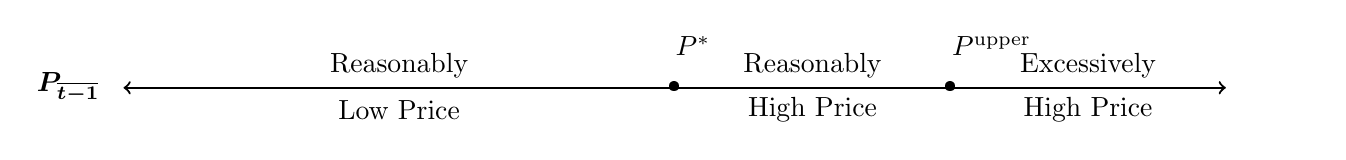
\begin{tikzpicture}[scale=7]

\node [draw=none] at (1.25,0.04) {Excessively};
\node [draw=none] at (1.25,-0.04) {High Price};

\node [draw=none] at (0.75,0.04) {Reasonably};
\node [draw=none] at (0.75,-0.04) {High Price};

\node [draw=none] at (0.0,0.04) {Reasonably};
\node [draw=none] at (0.0,-0.04) {Low Price};

\node [draw=none] at (0.533,0.075) {$P^{*}$};
\node [draw=none] at (1.075,0.075) {$P^{\text{upper}}$};

\foreach \Point in {0.5, 1}{
    \node[label={[label distance=1mm]:\rotatebox{0}{}}] at (\Point,0) {\textbullet};
}
\draw[thick,<->,color=black] (-0.5,0) -- (1.5,0); % Draw line
\node [draw=none] at (-0.6,0) {\bm{$P_{\overline{t-1}}$}}; % Chart label
\node [draw=none] at (1.6,0)  {\color{white} $P_{\overline{t-1}}$}; % Added to center chart

\end{tikzpicture}

\end{document}
    \vspace*{-7mm}
    \setlength{\belowcaptionskip}{-8pt} % reduce space after caption
    \caption{Price Level}
    \label{Price Level}
\end{figure}

%%%%%%%%%%%%%%%%%%%%%%%%%%%%%%% Debt Level %%%%%%%%%%%%%%%%%%%%%%%%%%%%%%%

\subsection{Debt Level}

The \term{Pod Rate} ($R^{D}$), such that $R^{D} \in \{j \times 10^{-6} \mid j \in \mathbb{N} \}$, represents the protocol debt level relative to the Pinto supply.

The protocol does not consider \term{Burnt} \Pinto, \term{Sown} \Pinto\  nor \term{Unharvestable Pods}, but does consider \term{Harvestable Pods}, as part of the total Pinto supply.

We define the total Pinto supply ($B$) for a given total Pinto minted over all \term{Seasons} ($M$), such that $B,\ M \in \{j \times 10^{-6} \mid j \in \mathbb{Z}^{+} \}$, total \term{Sown} \Pinto\ over all \term{Seasons} ($U$), and total \term{Burnt} \Pinto\ over all \term{Seasons} ($N$), such that $U,\ N \in \{j \times 10^{-6} \mid j \in \mathbb{N} \}$, as:

    $$
        B = M - (U + N)
    $$

We define $R^{D}$ for a given the total number of \term{Unharvestable Pods} ($D$), such that $D \in \{j \times 10^{-6} \mid j \in \mathbb{N} \}$, and $B$ as:

    $$
        R^{D} = \frac{D}{B}
    $$

\newpage

The protocol requires three $R^{D}$ levels to be set: (1) $R^{D^{\text{lower}}}$, (2) $R^{D^{*}}$, an optimal level of debt, and (3) $R^{D^{\text{upper}}}$, above or equal to which debt is considered excessively high, such that $R^{D^{*}},\ R^{D^{\text{upper}}} \in \{j \times 10^{-6} \mid j \in \mathbb{Z}^{+} \}$. When $R^{D^{\text{lower}}} \leq R^{D} < R^{D^{\text{upper}}}$ and $R^{D} \neq R^{D^{*}}$ (\textit{i.e.}, not optimal), $R^{D}$ is considered reasonable.

%%%%%%%%%%%%%%% Debt Level Figure %%%%%%%%%%%%%%%

\begin{figure}[h!]
    \centering
    \documentclass{standalone}
\usepackage{tikz,pgf}

\begin{document}

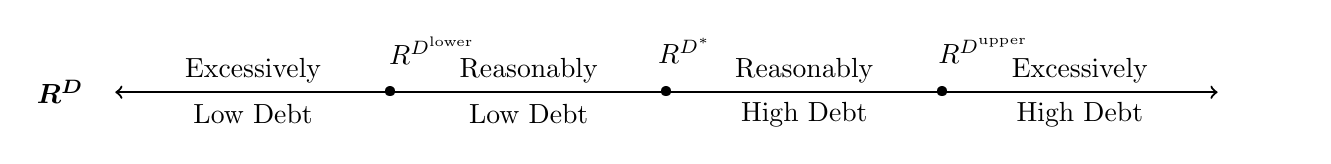
\begin{tikzpicture}[scale=7]

\node [draw=none] at (1.25,0.04) {Excessively};
\node [draw=none] at (1.25,-0.04) {High Debt};

\node [draw=none] at (0.75,0.04) {Reasonably};
\node [draw=none] at (0.75,-0.04) {High Debt};

\node [draw=none] at (0.25,0.04) {Reasonably};
\node [draw=none] at (0.25,-0.04) {Low Debt};

\node [draw=none] at (-0.25,0.04) {Excessively};
\node [draw=none] at (-0.25,-0.04) {Low Debt};

\node [draw=none] at (0.075,0.075) {$R^{D^{\text{lower}}}$};
\node [draw=none] at (0.533,0.075) {$R^{D^{*}}$};
\node [draw=none] at (1.075,0.075) {$R^{D^{\text{upper}}}$};

\foreach \Point in {0, 0.5, 1}{
    \node[label={[label distance=1mm]:\rotatebox{0}{}}] at (\Point,0) {\textbullet};
}
\draw[thick,<->,color=black] (-0.5,0) -- (1.5,0); % Draw line
\node [draw=none] at (-0.6,0) {\bm{$R^D$}}; % Chart label
\node [draw=none] at (1.6,0)  {\color{white} $R_D$}; % Added to center chart

\end{tikzpicture}

\end{document}
    \vspace*{-7mm}
    \setlength{\belowcaptionskip}{-8pt} % reduce space after caption
    \caption{Debt Level}
    \label{Debt Level}
\end{figure}

%%%%%%%%%%%%%%%%%%%%%%%%%%%%%%% Liquidity Level %%%%%%%%%%%%%%%%%%%%%%%%%%%%%%%

\subsection{Liquidity Level}

The \term{Liquidity Rate} ($R^{W}$), such that $R^{W} \in \{j \times 10^{-6} \mid j \in \mathbb{N} \}$, represents the protocol liquidity level relative to the Pinto supply.

The total non-Pinto USD-denominated value of liquidity in the \term{Silo} ($W$), such that $W \in \{j \times 10^{-6} \mid j \in \mathbb{N} \}$, is a function of $f^{\mathscr{W}^{\lambda}}$, the function to calculate the time weighted average non-Pinto USD-denominated value in a given number of \term{Deposited} $\lambda$ ($f^{\$}(z^{\lambda})$), such that $f^{\$}\colon \{j \times 10^{-\lambda} \mid j \in \mathbb{Z}^{+} \} \rightarrow \{j \times 10^{-18} \mid j \in \mathbb{Z}^{+} \}$, and $\mathbf{L}_{t}^{\lambda}$.

We define $f^{\$}(z^{\lambda})$ for a given inter-block MEV manipulation resistant TWA non-Pinto reserves in the Multi Flow \term{Pump}\fref{Any italicized terms not defined herein are defined by Pinto Exchange.} of $\lambda$ from the beginning of the previous \term{Season} to the current transaction ($\lambda_{\nonpinto,{t-1}_0,\Game}^{\text{SMA}}$), such that $\lambda_{\nonpinto,{t-1}_0,\Game}^{\text{SMA}} \in \{j \times 10^{-\nonpinto} \mid j \in \mathbb{Z}^{+} \}$, $f^{\$^{\lambda}}$, and the inter-block MEV manipulation resistant TWA number of $\lambda$ LP tokens from the beginning of the previous \term{Season} to the current transaction ($\lambda_{\lambda,{t-1}_0,\Game}^{\text{SMA}}$), such that $\lambda_{\lambda,{t-1}_0,\Game}^{\text{SMA}} \in \{j \times 10^{-\lambda} \mid j \in \mathbb{Z}^{+} \}$ as:

    $$
        f^{\$}(z^{\lambda}) = \frac{z^{\lambda} \times 
                                    \lambda_{\nonpinto,{t-1}_0,\Game}^{\text{SMA}} \times 
                                    f^{\$^{\lambda}}(3600)}
                                {\lambda_{\lambda,{t-1}_0,\Game}^{\text{SMA}}}
    $$

Therefore, we define $W$ for a given $f^{\mathscr{W}^{\lambda}}$, $f^{\$}(z^{\lambda})$ and $\mathbf{L}_{t}^{\lambda}$ as:

    $$
        W = \sum_{\lambda \in \Lambda \setminus \pinto} 
                    f^{\mathscr{W}^{\lambda}} \times 
                        f^{\$}(\mathbf{L}_{t}^{\lambda})
    $$

Therefore, we define $R^{W}$ for a given $W$ and $B$ as:

    $$
        R^{W} = \frac{W}{B}
    $$

\newpage 

The protocol requires three $R^{W}$ levels to be set: (1) $R^{W^{\text{lower}}}$, below which liquidity is considered excessively low, (2) $R^{W^{*}}$, an optimal level of liquidity, and (3) $R^{W^{\text{upper}}}$, above or equal to which liquidity is considered excessively high, such that $R^{W^{\text{lower}}},\ R^{W^{*}},\ R^{W^{\text{upper}}} \in \{j \times 10^{-6} \mid j \in \mathbb{Z}^{+} \}$. When $R^{W^{\text{lower}}} \leq R^{W} < R^{W^{\text{upper}}}$ and $R^{W} \neq R^{W^{*}}$ (\textit{i.e.}, not optimal), $R^{W}$ is considered reasonable.

\begin{figure}[h!]
    \centering
    \documentclass{standalone}
\usepackage{tikz,pgf}

\begin{document}

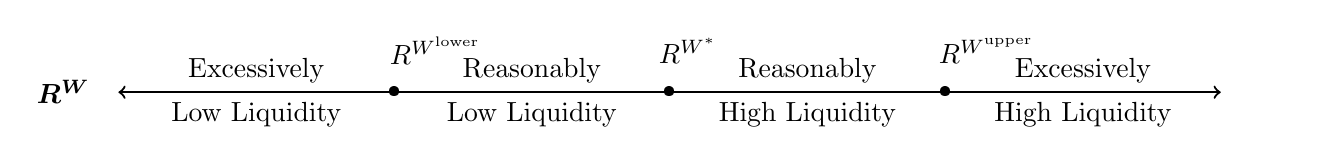
\begin{tikzpicture}[scale=7]

\node [draw=none] at (1.25,0.04) {Excessively};
\node [draw=none] at (1.25,-0.04) {High Liquidity};

\node [draw=none] at (0.75,0.04) {Reasonably};
\node [draw=none] at (0.75,-0.04) {High Liquidity};

\node [draw=none] at (0.25,0.04) {Reasonably};
\node [draw=none] at (0.25,-0.04) {Low Liquidity};

\node [draw=none] at (-0.25,0.04) {Excessively};
\node [draw=none] at (-0.25,-0.04) {Low Liquidity};

\node [draw=none] at (0.075,0.075) {$R^{W^{\text{lower}}}$};
\node [draw=none] at (0.533,0.075) {$R^{W^{*}}$};
\node [draw=none] at (1.075,0.075) {$R^{W^{\text{upper}}}$};

\foreach \Point in {0, 0.5, 1}{
    \node[label={[label distance=1mm]:\rotatebox{0}{}}] at (\Point,0) {\textbullet};
}
\draw[thick,<->,color=black] (-0.5,0) -- (1.5,0); % Draw line
\node [draw=none] at (-0.6,0) {\bm{$R^W$}}; % Chart label
\node [draw=none] at (1.6,0)  {\color{white} $R_W$}; % Added to center chart

\end{tikzpicture}

\end{document}
    \vspace*{-7mm}
    \setlength{\belowcaptionskip}{-8pt} % reduce space after caption
    \caption{Liquidity Level}
    \label{Liquidity Level}
\end{figure}

%%%%%%%%%%%%%%%%%%%%%%%%%%%%%%% Position %%%%%%%%%%%%%%%%%%%%%%%%%%%%%%%

\subsection{Position}

The position of the protocol with respect to ideal equilibrium can be represented on a graph with axes $R^{D}$, $R^{W}$ and $P$, and ideal equilibrium at the origin ($R^{D^{*}}$, $R^{W^{*}}$, $P^{*}$). The current state of the protocol is determined in part by the position of the protocol with respect to ideal equilibrium. 

%%%%%%%%%%%%%%% Position Figure %%%%%%%%%%%%%%%

\begin{figure}[h!]
    \centering
    \includegraphics[scale=.14]{./figures/Position} % change scale to change size
    \caption{Position}
    \label{Position}
\end{figure}

%%%%%%%%%%%%%%%%%%%%%%%%%%%%%%% Direction %%%%%%%%%%%%%%%%%%%%%%%%%%%%%%%

\subsection{Direction}
\vspace{0.1cm}

The position of the protocol with respect to ideal equilibrium changes at the beginning of each \term{Season}. The current state of the protocol with respect to ideal equilibrium is determined in part by the direction of this change. 

\vspace{0.1cm}

The direction of change in position of the protocol at the beginning of $t$ is considered either toward or away from ideal equilibrium, based on $R_{t-1}^{D}$ and $P_{\overline{t-1}}$. When $V < P_{\overline{t-1}}$ (\textit{i.e.}, $0 < \Delta B_{\overline{t-1}}$), debt is paid back; when $P_{\overline{t-1}} \leq V$ (\textit{i.e.}, $\Delta B_{\overline{t-1}} \leq 0$), debt can only increase or remain constant.

\vspace{0.1cm}

Therefore, when $R^{D^{*}} < R_{t-1}^{D}$ (\textit{i.e.}, there was more than optimal debt):

\vspace{0.1cm}

\begin{itemize}[topsep=0pt, itemsep=1pt]
    \item If $V < P_{\overline{t-1}}$, the protocol moves toward ideal equilibrium; and \vspace{0.1cm}
    \item If $P_{\overline{t-1}} \leq V$, the protocol moves away from ideal equilibrium.
\end{itemize}

\vspace{0.1cm}

When $R_{t-1}^{D} \leq R^{D^{*}}$ (\textit{i.e.}, there was less than optimal or optimal debt):

\begin{itemize}[topsep=0pt, itemsep=1pt]
    \item If $V < P_{\overline{t-1}}$, the protocol moves away from ideal equilibrium; or \vspace{0.1cm}
    \item If $P_{\overline{t-1}} \leq V$, the protocol moves toward ideal equilibrium.
\end{itemize}

\vspace{0.1cm}

%%%%%%%%%%%%%%% Direction Figure %%%%%%%%%%%%%%%

\begin{figure}[h!]
    \centering
    \advance\leftskip-1cm
    \includetable{Direction}
    \vspace*{2mm}
    \caption{Direction}
    \label{Direction}
\end{figure}

\vspace{0.1cm}

%%%%%%%%%%%%%%%%%%%%%%%%%%%%%%% Acceleration %%%%%%%%%%%%%%%%%%%%%%%%%%%%%%%

\vspace{0.1cm}
\subsection{Acceleration}
\vspace{0.1cm}

The current state of the protocol with respect to ideal equilibrium is also determined by the rate of change of direction of the protocol at the beginning of each \term{Season} (\textit{i.e.}, its acceleration).

\vspace{0.1cm}

The acceleration of the protocol is considered decelerating, steady or accelerating, based on $P_{\overline{t-1}}$, $R_{t-1}^{D}$ and changing demand for \term{Soil}. Demand for \term{Soil} is considered decreasing, steady or increasing. 

\vspace{0.1cm}

When demand for \term{Soil} is decreasing:

\vspace{0.1cm}

\begin{itemize}[topsep=0pt, itemsep=1pt]
    \item If $V < P_{\overline{t-1}}$, the protocol is decelerating; and \vspace{0.1cm}
    \item If $P_{\overline{t-1}} \leq V$, the protocol is accelerating.
\end{itemize}

\vspace{0.1cm}

When demand for \term{Soil} is steady, the protocol is steady.

\newpage 

When demand for \term{Soil} is increasing:

\begin{itemize}[topsep=0pt, itemsep=1pt]
    \item If $V < P_{\overline{t-1}}$, the protocol is accelerating; and
    \item If $P_{\overline{t-1}} \leq V$, the protocol is decelerating.
\end{itemize}

%%%%%%%%%%%%%%% Acceleration Figure %%%%%%%%%%%%%%%

\begin{figure}[h!]
    \centering
    \advance\leftskip-1.12cm
    \includetable{Acceleration}
    \vspace*{2mm}
    \setlength{\belowcaptionskip}{-8pt} % reduce space after caption
    \caption{Acceleration}
    \label{Acceleration}
\end{figure}

%%%%%%%%%%%%%%%%%%%%%%%%%%%%%%% Demand for Soil %%%%%%%%%%%%%%%%%%%%%%%%%%%%%%%

\vspace*{-3.5mm}
\subsection{Demand for Soil}
\vspace*{-3mm}

In order to properly classify its acceleration, the protocol must accurately measure changing demand for \term{Soil}.

The number of \term{Sown} \Pinto\ each \term{Season} ($u_{t}$), such that $u_{t} \in \{j \times 10^{-6} \mid j \in \mathbb{N} \}$, indicates demand for \term{Soil} over the course of that \term{Season}. The rate of change of $u_{t}$ from \term{Season} to \term{Season} ($\frac{\partial u_{t}}{\partial t}$), such that $\frac{\partial u_{t}}{\partial t} \in \{j \times 10^{-6} \mid j \in \mathbb{N} \}$, indicates changing demand for \term{Soil}.

We define $\frac{\partial u_{t}}{\partial t}$ over the previous two \term{Seasons}, $u_{t-1}$ and $u_{t-2}$, respectively, as:

    $$
        \frac{\partial u_{t}}{\partial t} = \frac{u_{t-1}}{u_{t-2}}
    $$

The protocol requires two $\frac{\partial u_{t}}{\partial t}$ levels to be set: (1) $\frac{\partial u_{t}}{\partial t}^{\text{lower}}$, below which demand for \term{Soil} is considered decreasing, and (2) $\frac{\partial u_{t}}{\partial t}^{\text{upper}}$, above or equal to which demand for \term{Soil} is considered increasing, such that $\frac{\partial u_{t}}{\partial t}^{\text{lower}},\ \frac{\partial u_{t}}{\partial t}^{\text{upper}} \in \{j \times 10^{-6} \mid j \in \mathbb{Z}^{+} \}$. When $\frac{\partial u_{t}}{\partial t}^{\text{lower}} \leq \frac{\partial u_{t}}{\partial t} < \frac{\partial u_{t}}{\partial t}^{\text{upper}}$, demand for \term{Soil} is considered steady.

%%%%%%%%%%%%%%% Soil Demand Changes From Derivative Figure %%%%%%%%%%%%%%%

\vspace*{-3.5mm}
\begin{figure}[h!]
    \centering
    \documentclass{standalone}
\usepackage{tikz,pgf}

\begin{document}

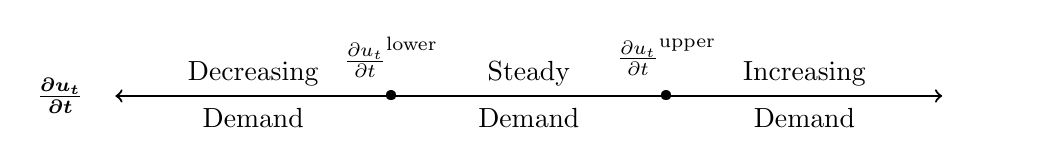
\begin{tikzpicture}[scale=7]

\node [draw=none] at (1,0.04) {Increasing};
\node [draw=none] at (1,-0.04) {Demand};

\node [draw=none] at (0.5,0.04) {Steady};
\node [draw=none] at (0.5,-0.04) {Demand};

\node [draw=none] at (0,0.04) {Decreasing};
\node [draw=none] at (0,-0.04) {Demand};

\node [draw=none] at (0.25,0.07) {$\frac{\partial u_t}{\partial t}^{\text{lower}}$};
\node [draw=none] at (0.75,0.07) {$\frac{\partial u_t}{\partial t}^{\text{upper}}$};

\foreach \Point in {0.25, 0.75}{
    \node[label={[label distance=1mm]:\rotatebox{0}{}}] at (\Point,0) {\textbullet};
}
\draw[thick,<->,color=black] (-0.25,0) -- (1.25,0); % Draw line
\node [draw=none] at (-0.35,0) {\bm{$\frac{\partial u_t}{\partial t}$}}; % Chart label
\node [draw=none] at (1.35,0)  {\color{white} $\frac{\partial u_t}{\partial t}$}; % Added to center chart

\end{tikzpicture}

\end{document}
    \vspace*{-10.5mm}
    \caption{Soil Demand Changes From $\frac{\partial u_{t}}{\partial t}$}
    \label{Soil Demand Changes From Derivative}
\end{figure}

However, when Pinto are \term{Sown} in all \term{Soil} in a \term{Season} (defined as $S_{t}^{\text{end}} \leq S^{\text{all}}$), $\frac{\partial u_{t}}{\partial t}$ can inaccurately measure changing demand for \term{Soil}. The first time Pinto are \term{Sown} in all \term{Soil} in a \term{Season}, after one or more \term{Seasons} where Pinto were not \term{Sown} in all \term{Soil}, demand for \term{Soil} is considered increasing. When Pinto are \term{Sown} in all \term{Soil} in consecutive \term{Seasons} (\textit{i.e.}, $t-1$ and $t-2$), the difference in time it took for the Pinto to be \term{Sown} in all \term{Soil} over the previous two \term{Seasons} ($\Delta E_{t}^{u}$), such that $\Delta E_{t}^{u} \in \mathbb{Z}$, can provide a more accurate measurement. 

In order to measure $\Delta E_{t}^{u}$, the protocol logs the time of the first \term{Sow} such that Pinto are \term{Sown} in all \term{Soil} in each \term{Season} ($\Delta E_{t}^{u^{\text{first}}}$), such that $\Delta E_{t}^{u^{\text{first}}} \in \mathbb{N}$, as the difference between the Base timestamp of the first \term{Sow} in $t$ such that there is at most one \term{Soil} ($E_{t}^{u^{\text{first}}}$) and $E_{\Xi}$. 

We define $\Delta E_{t}^{u^{\text{first}}}$ for a given $E_{t}^{u^{\text{first}}}$ and $E_{\Xi}$ as:

    $$
        \Delta E_{t}^{u^{\text{first}}} = 
            E_{t}^{u^{\text{first}}} - E_{\Xi}
    $$

If Pinto were \term{Sown} in all \term{Soil} in the first 20 minutes of the previous \term{Season} (\textit{i.e.}, $\Delta E_{t-1}^{u^{\text{first}}} < \Delta E_{t-1}^{u^{\text{first}^{\text{max}}}}$), demand for \term{Soil} is considered increasing. If Pinto were \term{Sown} in all \term{Soil} in both $t-1$ and $t-2$, but $\Delta E_{t-1}^{u^{\text{first}^{\text{max}}}} \leq \Delta E_{t-1}^{u^{\text{first}}}$, at the beginning of $t$ the protocol compares $\Delta E_{t-1}^{u^{\text{first}}}$ with $\Delta E_{t-2}^{u^{\text{first}}}$ to calculate $\Delta E_{t}^{u}$.

We define $\Delta E_{t}^{u}$ for a given $\Delta E_{t-1}^{u^{\text{first}}}$ and $\Delta E_{t-2}^{u^{\text{first}}}$ as:

    $$
        \Delta E_{t}^{u} = 
            \Delta E_{t-2}^{u^{\text{first}}} - \Delta E_{t-1}^{u^{\text{first}}}
    $$

If the above condition is met, changing demand for \term{Soil} is measured by $\Delta E_{t}^{u}$. the protocol requires two $\Delta E_{t}^{u}$ levels to be set: (1) $\Delta E_{t}^{u^{\text{lower}}}$, below which demand for \term{Soil} is considered decreasing, and (2) $\Delta E_{t}^{u^{\text{upper}}}$, above or equal to which demand for \term{Soil} is considered increasing, such that $\Delta E_{t}^{u^{\text{lower}}},\ \Delta E_{t}^{u^{\text{upper}}} \in \mathbb{Z}$. When $\Delta E_{t}^{u^{\text{lower}}} \leq \Delta E_{t}^{u} < \Delta E_{t}^{u^{\text{upper}}}$, demand for \term{Soil} is considered steady.

Thus, the protocol measures changing demand for \term{Soil}.

%%%%%%%%%%%%%%% Soil Demand Changes From Time Figure %%%%%%%%%%%%%%%

\begin{figure}[h!]
    \centering
    \documentclass{standalone}
\usepackage{tikz,pgf}

\begin{document}

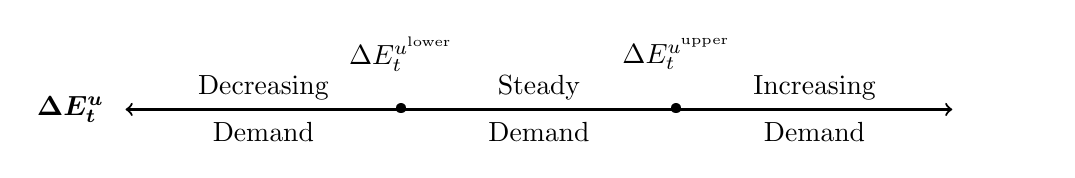
\begin{tikzpicture}[scale=7]

\node [draw=none] at (1,0.04) {Increasing};
\node [draw=none] at (1,-0.04) {Demand};

\node [draw=none] at (0.5,0.04) {Steady};
\node [draw=none] at (0.5,-0.04) {Demand};

\node [draw=none] at (0,0.04) {Decreasing};
\node [draw=none] at (0,-0.04) {Demand};

\node [draw=none] at (0.25,0.1) {$\Delta E_{t}^{u^{\text{lower}}}$};
\node [draw=none] at (0.75,0.1) {$\Delta E_{t}^{u^{\text{upper}}}$};

\foreach \Point in {0.25, 0.75}{
    \node[label={[label distance=1mm]:\rotatebox{0}{}}] at (\Point,0) {\textbullet};
}
\draw[thick,<->,color=black] (-0.25,0) -- (1.25,0); % Draw line
\node [draw=none] at (-0.35,0) {\bm{$\Delta E_{t}^{u}$}}; % Chart label
\node [draw=none] at (1.35,0)  {\color{white} $\Delta E_{t}^{u}$}; % Added to center chart

\end{tikzpicture}

\end{document}
    \vspace*{-10.5mm} % reduce space before caption
    \setlength{\belowcaptionskip}{-8pt} % reduce space after caption
    \caption{Soil Demand Changes From $\Delta E_{t}^{u}$}
    \label{Soil Demand Changes From Time}
\end{figure}

%%%%%%%%%%%%%%%%%%%%%%%%%%%%%%%%%%%%%%% Current State %%%%%%%%%%%%%%%%%%%%%%%%%%%%%%%%%%%%%%%

\subsection{Current State}

We define the current state of the protocol with respect to ideal equilibrium as the combination of its direction and acceleration with respect to ideal equilibrium. With two potential directions and three potential accelerations, the protocol has six potential current states:

\begin{multicols}{2}
\begin{itemize}[midsep]
    \item Accelerating away from ideal equilibrium;
    \item Steady away from ideal equilibrium;
    \item Decelerating away from ideal equilibrium;
    \item Accelerating toward ideal equilibrium;
    \item Steady toward ideal equilibrium; and
    \item Decelerating toward ideal equilibrium.
\end{itemize}
\end{multicols}

%%%%%%%%%%%%%%% Current State Figure %%%%%%%%%%%%%%%

\begin{figure}[h!]
    \centering
    \advance\leftskip-1cm
    \includetable{Current-State}
    \vspace*{0mm}
    \setlength{\belowcaptionskip}{-8pt} % reduce space after caption
    \caption{Current State}
    \label{Current State}
\end{figure}

%%%%%%%%%%%%%%%%%%%%%%%%%%%%%%%%%%%%%%% Optimal State %%%%%%%%%%%%%%%%%%%%%%%%%%%%%%%%%%%%%%%

\newpage

\subsection{Optimal State}

An optimal state of the protocol is an optimal current state and determined by $R_{t-1}^{D}$.

We define an optimal state of the protocol as accelerating toward ideal equilibrium, or either steady or decelerating toward ideal equilibrium. When $R_{t-1}^{D}$ is excessively high or low, the optimal state is accelerating toward ideal equilibrium. When $R_{t-1}^{D}$ is reasonably high or low, the optimal state is either steady or decelerating toward ideal equilibrium.

%%%%%%%%%%%%%%% Optimal State Figure %%%%%%%%%%%%%%%

\begin{figure}[h!]
    \centering
    \advance\leftskip-1cm
    \includetable{Optimal-State}
    \vspace*{2mm}
    \setlength{\belowcaptionskip}{-8pt} % reduce space after caption
    \caption{Optimal State}
    \label{Optimal State}
\end{figure}

%%%%%%%%%%%%%%%%%%%%%%%%%%%%%%%%%%%%%%% Pinto Supply %%%%%%%%%%%%%%%%%%%%%%%%%%%%%%%%%%%%%%%

\subsection{Pinto Supply}

At the beginning of each \term{Season}, if $V < P_{\overline{t-1}}$, the protocol increases the Pinto supply based on $\Delta B_{\overline{t-1}}$ in addition to the reward for successfully calling the \code{gm} function. Up to 48.5\% of the additional Pinto supply increase is used to pay off \term{Pods}, up to 3\% of the additional Pinto supply increase is distributed to the Pinto development budget\fref{basescan.org/address/0xb0cdb715D8122bd976a30996866Ebe5e51bb18b0} or to repay Beanstalk debt\fref{pinto.money/repay-beanstalk-debt}, and the remainder is distributed to \term{Stalkholders}. If the Pinto supply is less than 1 billion, 3\% is distributed to the Pinto development budget. If the Pinto supply is greater than 1 billion, up to 3\% is distributed to repay Beanstalk debt.

At the beginning of each \term{Season}, the protocol mints $m_{t}$ Pinto, such that $m_{t} \in \{j \times 10^{-6} \mid j \in \mathbb{Z}^{+} \}$.

We define $m_{t}$ for a given $\Delta B_{\overline{t-1}}$ and $a_{t}$ as:

    $$
        m_{t} = 
            \text{max}(0,\ \Delta B_{\overline{t-1}}) + a_{t}
    $$

The distribution of the additional mint is dependent on $\Delta B_{\overline{t-1}}$, $D$ and $B$. If $0 < \frac{\Delta B_{\overline{t-1}}\ \times\ 485}{1000} < D$ (\textit{i.e.}, there are at least $\frac{\Delta B_{\overline{t-1}}\ \times\ 485}{1000}$ \term{Unharvestable Pods}), $\frac{\Delta B_{\overline{t-1}}\ \times\ 485}{1000}$ \term{Pods} \term{Ripen} and become \term{Harvestable}, up to $\frac{\Delta B_{\overline{t-1}}\ \times\ 30}{1000}$ newly minted Pinto are distributed to the Pinto development budget or to repay Beanstalk debt, and the remaining newly minted Pinto are distributed to \term{Stalkholders}. If $0 < D < \frac{\Delta B_{\overline{t-1}}\ \times\ 485}{1000}$ (\textit{i.e.}, there are less \term{Unharvestable Pods} than $\frac{\Delta B_{\overline{t-1}}\ \times\ 485}{1000}$), $D$ \term{Pods} \term{Ripen} and become \term{Harvestable}, up to $\frac{\Delta B_{\overline{t-1}}\ \times\ 30}{1000}$ newly minted Pinto are distributed to the Pinto development budget or to repay Beanstalk debt, and the remaining newly minted Pinto are distributed to \term{Stalkholders}.

\newpage

In a \term{Flood} (defined below), the number of \term{Pods} that \term{Ripen} and become \term{Harvestable} at the beginning of each \term{Season} ($\Delta D_{t}$), such that $\Delta D_{t} \in \{j \times 10^{-6} \mid j \in \mathbb{N} \}$, is based on the maximum percent of the Pinto supply worth of \term{Pods} that become \term{Harvestable} during a \term{Flood} ($D^{F}$), such that $D^{F} \in \{j \times 10^{-6} \mid j \in \mathbb{N} \}$.

Therefore, we define $\Delta D_{t}$ for a given $\Delta B_{\overline{t-1}}$, $B$, $D^{F}$ and $D$ as:

    $$
        \Delta D_{t} =
            \begin{cases}
               {\text{min}\left(
                    \frac{\Delta B_{\overline{t-1}}\ \times\ 485}
                            {1000} + B \times D^{F},\ 
                        D\right)}\
                    & \text{if } \term{Flooding} \\

               {\text{min}\left(
                    \text{max}\left
                        (0,\ 
                        \frac{\Delta B_{\overline{t-1}}\ \times\ 485}
                                {1000}\right),\ 
                            D\right)}
                    & \text{else }   
            \end{cases}
    $$

%%%%%%%%%%%%%%%%%%%%%%%%%%%%%%%%%%%%%%% Soil Supply %%%%%%%%%%%%%%%%%%%%%%%%%%%%%%%%%%%%%%%

\subsection{Soil Supply}

Pinto is willing to issue debt every \term{Season}. When $V \leq P_{\overline{t-1}}$, the \term{Soil} supply is based on (1) the number of \term{Pods} that \term{Ripen} and became \term{Harvestable} at the beginning of the \term{Season}, (2) the \term{Temperature} in each interval of the \term{Morning} of $t$ ($h_{t_{q}}$), such that $h_{t_{q}} \in \{j \times 10^{-6} \mid j \in \mathbb{Z}^{+} \}$, and (3) the \term{Till Scalar} ($\mathscr{P}$), such that $\mathscr{P} \in \{j \times 10^{-18} \mid j \in \mathbb{Z}^{+} \}$. When $P_{\overline{t-1}} < V$, the \term{Soil} supply is also based on (4) the sum of shortages and excesses of Pinto across liquidity pools on the \term{Minting Whitelist} calculated using the inter-block MEV manipulation resistant instantaneous reserves in Multi Flow \term{Pump} ($\Delta B_{\Xi-1}^{\text{EMA}}$), such that $\Delta B_{\Xi-1}^{\text{EMA}} \in \{j \times 10^{-6} \mid j \in \mathbb{Z} \}$, (5) $\Delta B_{\overline{t-1}}$, (6) the \term{Furrow Scalar} ($\mathscr{F}$), such that $\mathscr{F} \in \{j \times 10^{-18} \mid j \in \mathbb{Z} \}$, (7) $W$, (8) the \term{Soil Diffusion Period} ($\mathscr{R}$), such that $\mathscr{R} \in \mathbb{Z}^{+}$, (9) the \term{Cultivation Factor} during $t$ ($\mathfrak{C}_{t}$), such that $\mathfrak{C}_{t} \in \{j \times 10^{-6} \mid j \in \mathbb{Z}^{+} \}$, and (10) the minimum \term{Soil} issued ($\overline{S}^{\text{min}}$), such that $\overline{S}^{\text{min}} \in \{j \times 10^{-6} \mid j \in \mathbb{Z}^{+} \}$.

We define the \term{Till Scalar} for a given $R^{D^{\text{upper}}}$, $R_{t-1}^{D}$, $R^{D^{*}}$ and $R^{D^{\text{lower}}}$ as:

    $$
        \mathscr{P} = 
            \begin{cases} 
                0.25
                    & \text{if} \; R^{D^{\text{upper}}} \leq R_{t-1}^{D} \vspace{.3cm} \\ 

                0.5
                    & \text{if} \; R^{D^{*}} \leq R_{t-1}^{D} < R^{D^{\text{upper}}} \vspace{.3cm} \\ 
                    
                1
                    & \text{if} \; R^{D^{\text{lower}}} \leq R_{t-1}^{D} < R^{D^{*}} \vspace{.3cm} \\ 
                    
                1.2
                    & \text{else} 
            \end{cases}
    $$

We define $S_{t_{q}}^{\text{min}}$ for a given $f^{\mathscr{P}}(R_{t-1}^{D})$, $\Delta D_{t}$ and $h_{t_{q}}$ as:

\vspace*{2mm}

    $$
        S_{t_{q}}^{\text{min}} = 
            \dfrac{\mathscr{P} \times \Delta D_{t}}
                    {1 + \frac{h_{t_{q}}}
                                {100}}
    $$

\vspace*{2mm}

The protocol calculates the \term{Maximum Soil} ($S_{t_{q}}^{\text{max}}$), such that $S_{t_{q}}^{\text{max}} \in \{j \times 10^{-6} \mid j \in \mathbb{N} \}$, in each interval $q$ of the \term{Morning} of $t$ for a given $\Delta B_{\Xi-1}^{\text{EMA}}$, $\Delta B_{\overline{t-1}}$, $\mathscr{F}$, $W$, $\mathscr{R}$, $\mathfrak{C}_{t}$, $\overline{S}^{\text{min}}$, $\mathscr{P}$ and $S_{t_{q}}^{\text{min}}$ as:

    \begin{adjustwidth}{-2cm}{-2cm}
    $$
        S_{t_{q}}^{\text{max}} = 
            \begin{cases} 
                \text{max}(\text{min}(-\Delta B_{\Xi-1}^{\text{EMA}}, -\Delta B_{\overline{t-1}}) \times \mathscr{F} \times \text{min}(0.01, 1 - W) \times \frac{1}{\mathscr{R}} \times \mathfrak{C}_{t}, \overline{S}^{\text{min}})
                    & \text{if} \; 
                        \Delta B_{\overline{t-1}} < 0 \mkern6mu \&\& \mkern6mu \Delta B_{\Xi-1}^{\text{EMA}} < 0 \\

                \mathscr{P} \times \frac{-\Delta B_{\overline{t-1}}}{100}
                    & \text{if} \; 
                        \Delta B_{\overline{t-1}} < 0 \mkern6mu \&\& \mkern6mu \Delta B_{\Xi-1}^{\text{EMA}} > 0 \\
                
                S_{t_{q}}^{\text{min}}
                    & \text{else} 
            \end{cases} 
    $$
    \end{adjustwidth}

%%%%%%%%%%%%%%%%%%%%%%%%%%%%%%%%%%%%%%% Temperature %%%%%%%%%%%%%%%%%%%%%%%%%%%%%%%%%%%%%%%

\newpage

\subsection{Temperature}
\vspace*{1.4mm}

The protocol attempts to regularly cross the price of \Pinto1 over its value target during long run decreases and increases in demand for Pinto by adjusting the \term{Maximum Temperature} in an attempt to maintain an optimal state, or to move from its current state into an optimal state. During the \term{Morning} of each \term{Season}, a Dutch auction determines the \term{Temperature} increases at the beginning of each interval. 

%%%%%%%%%%%%%%%%%%% Maximum Temperature %%%%%%%%%%%%%%%%%%%

\vspace*{1.4mm}
\subsubsection{Maximum Temperature}
\vspace*{1.4mm}

The \term{Maximum Temperature} change at the beginning of $t$ is determined by $R_{t-1}^{D}$, $R_{t-1}^{W}$, $P_{\overline{t-1}}$ and changing demand for \term{Soil}.

\vspace*{1.4mm}

The protocol changes the \term{Maximum Temperature} in both a relative ($H^{m}$), such that $H^{m} \in \{j \times 10^{-6} \mid j \in \mathbb{N} \}$, and absolute manner ($H^{b}$), such that $H^{b} \in \mathbb{Z}$, at the beginning of $t$ as:

\vspace*{1.4mm}

    $$
        H_{t} = \text{max}(
                    H^{m} \times H_{t-1} + H^{b}, 
                    1)
    $$

\vspace*{1.4mm}

$H^{m}$ and $H^{b}$ are shown in Figures 13, 14, 15 and 16 as ($H^{m}$, $H^{b}$).

\vspace*{1.4mm}

%%%%%%%%%%%%%% Maximum Temperature Change Figures %%%%%%%%%%%%%%

\begin{figure}[h!]
    \centering
    \advance\leftskip-1cm
    \includetable{Max-Temp-Changes-Excessively-Low-Liquidity}
    \vspace*{2mm}
    \caption{Maximum Temperature Changes From $P_{\overline{t-1}}$, Demand for Soil Changes and $R_{t-1}^{D}$ with an Excessively Low $R_{t-1}^{W}$}
    \label{Max Temp Changes Excessively Low Liquidity}
\end{figure}

\begin{figure}[h!]
    \centering
    \advance\leftskip-1cm
    \includetable{Max-Temp-Changes-Reasonably-Low-Liquidity}
    \vspace*{2mm}
    \caption{Maximum Temperature Changes From $P_{\overline{t-1}}$, Demand for Soil Changes and $R_{t-1}^{D}$ with a Reasonably Low $R_{t-1}^{W}$}
    \label{Max Temp Changes Reasonably Low Liquidity}
\end{figure}

\begin{figure}[h!]
    \centering
    \advance\leftskip-1cm
    \includetable{Max-Temp-Changes-Reasonably-High-Liquidity}
    \vspace*{2mm}
    \caption{Maximum Temperature Changes From $P_{\overline{t-1}}$, Demand for Soil Changes and $R_{t-1}^{D}$ with a Reasonably High $R_{t-1}^{W}$}
    \label{Max Temp Changes Reasonably High Liquidity}
\end{figure}

\clearpage

\begin{figure}[h!]
    \centering
    \advance\leftskip-1cm
    \includetable{Max-Temp-Changes-Excessively-High-Liquidity}
    \vspace*{2mm}
    \caption{Maximum Temperature Changes From $P_{\overline{t-1}}$, Demand for Soil Changes and $R_{t-1}^{D}$ with an Excessively High $R_{t-1}^{W}$}
    \label{Max Temp Changes Excessively High Liquidity}
\end{figure}

%%%%%%%%%%%%%%%%%%% Morning %%%%%%%%%%%%%%%%%%%

\subsubsection{Morning}
\vspace{-0.025cm}

The \term{Temperature} increases logarithmically in each interval of the \term{Morning} of $t$ based on $H_{t}$, the number of intervals in the \term{Morning} ($\mathfrak{Q}$), such that $\mathfrak{Q} \in \mathbb{Z}^{+}$, and a control variable ($\sigma$), such that $\sigma \in \{j \times 10^{-\infty} \mid j \in \mathbb{Z}^{+} \}$, as:

\vspace{-0.025cm}

    $$ 
        h_{t_{q}} =
            \begin{cases}
                \text{max}(
                        H_{t}*\text{log}_{\mathfrak{Q}\sigma + 1}(q\sigma + 1),\ 
                        \frac{H_{t}}{100})
                    & \text{if} \; q < \mathfrak{Q} \\
                    
                H_{t} 
                    & \text{else}
            \end{cases} 
    $$

\vspace{-0.025cm}

Thus, the protocol changes the \term{Temperature} in an attempt to regularly cross the price of \Pinto1 over its value target during long run decreases and increases in demand for Pinto.

%%%%%%%%%%%%%%%%%%%%%%%%%%%%%%%%% Crop Ratio %%%%%%%%%%%%%%%%%%%%%%%%%%%%%%%%%

\vspace{-0.025cm}
\subsection{Crop Ratio}
\vspace{-0.025cm}

The protocol attempts to regularly cross the price of \Pinto1 over its value target during long run decreases and increases in demand for Pinto by adjusting the \term{Crop Ratio}. In practice, the protocol adjusts the \term{Crop Ratio} by changing the \term{Crop Scalar}. The \term{Crop Scalar} change at the beginning of $t$ is determined by $R_{t-1}^{D}$, $R_{t-1}^{W}$, $P_{\overline{t-1}}$ and changing demand for \term{Soil}. 

\vspace{-0.025cm}

The protocol changes the \term{Crop Scalar} in both a relative ($\mathscr{X}^{m}$), such that $\mathscr{X}^{m} \in \{j \times 10^{-18} \mid j \in \mathbb{N} \}$, and absolute manner ($\mathscr{X}^{b}$), such that $\mathscr{X}^{b} \in \{j \times 10^{-18} \mid j \in \mathbb{Z} \}$, at the beginning of $t$ as:

\vspace{-0.025cm}

$$
    \mathscr{X}_{t} = \text{min}(
                        \text{max}(
                            \mathscr{X}^{m} \times \mathscr{X}_{t-1} + \mathscr{X}^{b}, 
                            0), 
                        1)
$$

\vspace{-0.025cm}

$\mathscr{X}^{m}$ and $\mathscr{X}^{b}$ are shown in Figures 17, 18, 19 and 20 as ($\mathscr{X}^{m}$, $\mathscr{X}^{b}$).

%%%%%%%%%%%%%%%%%%% Crop Scalar Change Figures %%%%%%%%%%%%%%%%%%%

\begin{figure}[h!]
    \centering
    \advance\leftskip-1cm
    \includetable{Crop-Scalar-Changes-Excessively-Low-Liquidity}
    \vspace*{2mm}
    \caption{Crop Scalar Changes From $P_{\overline{t-1}}$, Demand for Soil Changes and $R_{t-1}^{D}$ with an Excessively Low $R_{t-1}^{W}$}
    \label{Crop Scalar Changes Excessively Low Liquidity}
\end{figure}

\begin{figure}[h!]
    \centering
    \advance\leftskip-1cm
    \includetable{Crop-Scalar-Changes-Reasonably-Low-Liquidity}
    \vspace*{2mm}
    \caption{Crop Scalar Changes From $P_{\overline{t-1}}$, Demand for Soil Changes and $R_{t-1}^{D}$ with a Reasonably Low $R_{t-1}^{W}$}
    \label{Crop Scalar Changes Reasonably Low Liquidity}
\end{figure}

\clearpage

\begin{figure}[h!]
    \centering
    \advance\leftskip-1cm
    \includetable{Crop-Scalar-Changes-Reasonably-High-Liquidity}
    \vspace*{2mm}
    \caption{Crop Scalar Changes From $P_{\overline{t-1}}$, Demand for Soil Changes and $R_{t-1}^{D}$ with a Reasonably High $R_{t-1}^{W}$}
    \label{Crop Scalar Changes Reasonably High Liquidity}
\end{figure}

\begin{figure}[h!]
    \centering
    \advance\leftskip-1cm
    \includetable{Crop-Scalar-Changes-Excessively-High-Liquidity}
    \vspace*{2mm}
    \caption{Crop Scalar Changes From $P_{\overline{t-1}}$, Demand for Soil Changes and $R_{t-1}^{D}$ with an Excessively High $R_{t-1}^{W}$}
    \label{Crop Scalar Changes Excessively High Liquidity}
\end{figure}

%%%%%%%%%%%%%%%%%%%%%%%%%%%%%% Flood %%%%%%%%%%%%%%%%%%%%%%%%%%%%%%

\vspace{-0.15cm}
\subsection{Flood}
\vspace{-0.15cm}

During long run increases in demand for Pinto, at the beginning of each \term{Season}, the protocol sells newly minted Pinto on the open market if increasing the Pinto supply, lowering the \term{Maximum Temperature} and lowering the \term{Crop Ratio} have not crossed the average nor current prices of \Pinto1 over its value target.

\vspace{-0.05cm}

If $V < P_{\overline{t-1}}$ and $R_{t-1}^{D} < R^{D^{\text{lower}}}$, it is \term{Raining}. If it has \term{Rained} for $F$, such that $F \in \mathbb{Z}^{+}$, consecutive full \term{Seasons} and at the beginning of the next \term{Season} it is still \term{Raining}, it \term{Floods}. 

\vspace{-0.05cm}

At the beginning of each \term{Season} in which it \term{Floods}, the protocol mints additional Pinto and sells them directly in the pools on the \term{Flood Whitelist} with the highest shortage of Pinto at the end of the previous \term{Season}. Proceeds from the sale are distributed to \term{Stalkholders} at the beginning of $t$ in proportion to their \term{Stalk} holdings when it began to \term{Rain} that they still have. At the beginning of each \term{Season} in which it Floods, up to 0.1\% of the Pinto supply worth of \term{Pods} that grew from Pinto \term{Sown} before it began to \term{Rain} \term{Ripen} and become \term{Harvestable}.

\vspace{-0.05cm}

The number of Pinto that are minted and sold to return the price of \Pinto1 to its value target is calculated from the sum of differences between the optimal number of Pinto and the number of Pinto in each liquidity pool on the \term{Flood Whitelist} in the current transaction ($\Delta B_{\Game}$), such that $\Delta B_{\Game} \in \{j \times 10^{-6} \mid j \in \mathbb{Z} \}$. For each marginal Pinto minted to be sold, the protocol sells it into the pool with the highest shortage of Pinto until all Pinto are sold.

\vspace{-0.05cm}

In a \term{Flood}, $m_{t}$ for a given $D$, $B$, $D^{F}$, $a_{t}$, $\Delta B_{\overline{t-1}}$ and $\Delta B_{\Game}$ is:

\vspace{-0.05cm}

    $$
        m_{t} = 
            \text{min}(D, B \times D^{F}) + 
            a_{t} + 
            \Delta B_{\overline{t-1}} + 
            \Delta B_{\Game}
    $$

\vspace{-0.05cm}

Thus, the protocol attempts to regularly cross the price of \Pinto1 over its value target during both long run increases and decreases in demand for Pinto.

%%%%%%%%%%%%%%%%%%%%%%%%%%%%%%%%%%%%%%%%%%%%%%   Toolshed   %%%%%%%%%%%%%%%%%%%%%%%%%%%%%%%%%%%%%%%%%%%%%%

\section{Toolshed}
\vspace{0.1cm}

The \term{Toolshed} offers a suite of tools that decrease friction to using the protocol and participating in peg maintenance.

%%%%%%%%%%%%%%%%%%%%%%%%%%%%%% Pod Market %%%%%%%%%%%%%%%%%%%%%%%%%%%%%%

\vspace{0.1cm}
\subsection{Pod Market}
\vspace{0.1cm}

The \term{Pod Market} is a peer-to-peer marketplace that allows \term{Pods} to be bought and sold in a trustless fashion without trading fees. Specifications of the \term{Pod Market} are outside the scope of this whitepaper. For information on the \term{Pod Market}, refer to the Appendix.

%%%%%%%%%%%%%%%%%%%%%%%%%%%%%% Depot %%%%%%%%%%%%%%%%%%%%%%%%%%%%%%

\vspace{0.1cm}
\subsection{Depot}
\vspace{0.1cm}

Complex interactions with Base-native protocols can be tedious, cumbersome and expensive. The \term{Depot} facilitates complex, gas-efficient interactions with other Base-native protocols in a single transaction. Any external protocol with a \term{Pipeline} to the \term{Depot} can be used through the protocol in a single transaction. \term{Pipelines} to the \term{Depot} can be added and removed via the \term{PCM}. The specifications of specific \term{Pipelines} are outside the scope of this whitepaper. For information on the \term{Depot}, refer to the Appendix.

%%%%%%%%%%%%%%%%%%%%%%%% Farm Balances %%%%%%%%%%%%%%%%%%%%%%%%

\vspace{0.1cm}
\subsection{Farm Balances}
\vspace{0.1cm}

\term{Farm Balances} are assets stored on the \term{Farm} that are not \term{Deposited} in the \term{Silo} or locked in \term{Pod Orders}. \term{Farm Balances} enable the protocol to store any ERC-20 token on behalf of a user.

All interactions with the protocol that use a user's ERC-20 tokens can use tokens from both \term{Farm} and \term{Wallet Balances}.

%%%%%%%%%%%%%%%%%%%%%%%% Tractor %%%%%%%%%%%%%%%%%%%%%%%%

\vspace{0.1cm}
\subsection{Tractor}
\vspace{0.1cm}

\term{Tractor} is a peer-to-peer transaction marketplace that allows third parties to perform pre-authorized actions through the protocol on behalf of a user. Specifications of \term{Tractor} are outside the scope of this whitepaper.

%%%%%%%%%%%%%%%%%%%%%%%%%%%%%%%%%%%%%%   Economics   %%%%%%%%%%%%%%%%%%%%%%%%%%%%%%%%%%%%%%

\vspace{0.1cm}
\section{Economics}
\vspace{0.1cm}

The protocol is designed from economic first principles to increase trustlessness, stability and liquidity over time.

%%%%%%%%%%%%%%% Ownership Concentration %%%%%%%%%%%%%%%

\vspace{0.1cm}
\subsection{Ownership Concentration}
\vspace{0.1cm}

A design that lowers the Gini coefficient\fref{wikipedia.org/wiki/Gini\_coefficient} of Pinto and \term{Stalk} over time is essential to censorship resistance.

\vspace{0.1cm}

Older \term{Deposits} have their \term{Stalk} diluted relative to newer \term{Deposits} every \term{Season}. Therefore, newly minted Pinto are more widely distributed over time.

\vspace{0.1cm}

The protocol does not require a pre-mine. The first 1000 Pinto are created when the \code{init} function is called to deploy the protocol.

%%%%%%%%%%%%%%% Strong Credit %%%%%%%%%%%%%%%

\vspace{0.1cm}
\subsection{Strong Credit}
\vspace{0.1cm}

Pinto is credit based and only fails if it can no longer attract creditors. A reasonable level of debt, strong credit history, competitive interest rate and reasonable level of liquidity attract creditors. 

\vspace{0.1cm}

The protocol attempts to change the \term{Temperature} and \term{Crop Ratio} to return $R^{D}$ to $R^{D^{*}}$ while regularly crossing the price of \Pinto1 over its value target. The protocol acts more aggressively when $R^{D}$ is excessively high or low.

\vspace{0.1cm}

The protocol never defaults on debt and is willing to issue \term{Pods} every \term{Season}. 

%%%%%%%%%%%%%%% Deep Liquidity %%%%%%%%%%%%%%%

\vspace{0.1cm}
\subsection{Deep Liquidity}
\vspace{0.1cm}

The value of \Pinto\ is derived from the liquidity they trade against. Reasonable levels of debt and liquidity attract more liquidity. 

\vspace{0.1cm}

The protocol attempts to change the \term{Temperature} and \term{Crop Ratio} to return $R^{W}$ to $R^{W^{*}}$ while regularly crossing the price of \Pinto1 over its value target. The protocol acts more aggressively when $R^{W}$ is excessively high or low.

\newpage

%%%%%%%%%%%%%%% Marginal Rate of Substitution %%%%%%%%%%%%%%%

\subsection{Marginal Rate of Substitution}

There are a wide variety of opportunities Pinto has to compete with for creditors and liquidity providers. Therefore, the protocol does not define an optimal \term{Temperature} or \term{Crop Ratio}, but instead adjusts them to move closer to ideal equilibrium. 

%%%%%%%%%%%%%%% Low Friction %%%%%%%%%%%%%%%

\subsection{Low Friction}

Minimizing the cost of using Pinto and barriers to the \term{Farm} maximizes utility for users and appeal to creditors. The \term{Depot} realizes the benefits of composability on Base.

The FIFO \term{Pod} \term{Harvest} schedule allows smaller \term{Sowers} to participate in peg maintenance and decreases the benefit of large scale price manipulation. The combination of non-expiry, the FIFO \term{Harvest} schedule, the Dutch auction, transferability, a liquid secondary market and \term{Tractor} enables \term{Sowers} to \term{Sow} Pinto as efficiently as possible. By maximizing the efficiency of the \term{Soil} market, Pinto minimizes its cost to attract creditors, the durations and magnitudes of price deviations below its value target, and excess \term{Pod} issuance.

%%%%%%%%%%%%%%% Equilibrium %%%%%%%%%%%%%%%

\subsection{Equilibrium}
\vspace{-0.15cm}

Equilibrium is a state of equivalent marginal quantity supplied and demanded. The protocol affects the supply of and demand for Pinto in attempt to regularly cross the equilibrium price of \Pinto1 over its value target. 

\vspace{-0.15cm}

While the protocol can arbitrarily increase the Pinto supply when the equilibrium price of \Pinto1 is above its value target, it cannot arbitrarily decrease the Pinto supply when the equilibrium price of \Pinto1 is below it. The protocol relies on the codependence between the equilibria of Pinto and \term{Soil} to work around this limitation. 

%%%%%%%%%%%%%%% Incentives %%%%%%%%%%%%%%%

\vspace{-0.15cm}
\subsection{Incentives}
\vspace{-0.15cm}

Protocol-native financial incentives are designed to increase trustlessness, stability and liquidity over time by coordinating independently financially motivated actors (\textit{i.e}, \term{Stalkholders} and \term{Sowers}). 

\vspace{-0.15cm}

The \term{Stalk} and \term{Seed Gauge Systems} incentivize (1) \term{Depositing} assets in the \term{Silo}, (2) leaving assets \term{Deposited} in the \term{Silo} continuously by creating opportunity cost to \term{Withdraw} assets from the \term{Silo}, (3) adding value to liquidity pools with Pinto by rewarding at least as many \term{Seeds} to at least one \term{Deposited} LP token as \term{Deposited} \Pinto, and (4) returning the price of \Pinto1 to its value target by allowing \term{Conversions} within the \term{Silo} without forfeiting \term{Stalk}.

\vspace{-0.15cm}

When $V < P_{\overline{t}}$, there is an incentive to buy Pinto to earn a portion of the upcoming Pinto seigniorage. This is exacerbated when $R^{D}$ is lower and $R^{W}$ is higher. The \term{Germination} period reduces this incentive significantly. The combination of the commitment to (1) automatically return the price of \Pinto1 to its value target and (2) distribute proceeds from the sale to current \term{Stalkholders} based on \term{Stalk} ownership when it began to \term{Rain}, removes this incentive entirely during \term{Seasons} where it is \term{Raining}.

\vspace{-0.15cm}

Thus, the protocol is designed to consistently increase trustlessness, stability and liquidity over time.

%%%%%%%%%%%%%%%%%%%%%%%%%%%%%%%%%%%%%%%%%%   Risk   %%%%%%%%%%%%%%%%%%%%%%%%%%%%%%%%%%%%%%%%%%

\vspace{-0.15cm}
\section{Risk}
\vspace{-0.15cm}

There are numerous risks associated with Pinto.\fref{docs.pinto.money/disclosures} This is not an exhaustive list.

\vspace{-0.15cm}

The protocol code base and peg maintenance mechanism are novel. Neither had been tested in the “real world” prior to the initial protocol deployment. Portions of the Pinto code base are unaudited.\footnote{\href{https://docs.pinto.money/resources/audits}{docs.pinto.money/resources/audits}} The open source nature of Pinto means that anyone can take advantage of any bugs, flaws or deficiencies in Pinto and launch identical or very similar low-volatility money implementations.

\vspace{-0.15cm}

A trustless implementation of Pinto has four external dependencies:

\begin{enumerate}[label=(\arabic*)]
    \item A trustless computer network that supports composability and both fungible and semi-fungible token standards (\textit{e.g.}, Base and the ERC-20 and ERC-1155 Standards, respectively);
    \item A trustless exchange protocol with an inter-block MEV manipulation resistant oracle that runs on (1) (\textit{e.g.}, Pinto Exchange\fref{pinto.exchange} and Multi Flow, respectively); 
    \item A liquid, trustless network-native asset with endogenous value (\textit{e.g.}, ETH); and
    \item A trustless oracle for the value of (3) in $V$, or a non-network-native exogenous value convertible stablecoin protocol native to (1) that offers convertibility to its non-network-native exogenous value collateral (\textit{e.g.}, USDC, USDT) that trades on (2) against (3) with sufficient liquidity.
\end{enumerate}

The current implementation of Pinto lacks (4) and has three additional external dependencies: 

\begin{enumerate}[label=(\arabic*), start=5]
    \item The non-network-native assets in each $\lambda$ on the \term{Deposit Whitelist};
    \item Non-network-native data feeds that facilitate reading inter-block MEV manipulation resistant USD-denominated prices of (3) and (5) (\textit{e.g.}, the ETH/USD\fref{data.chain.link/feeds/base/base/eth-usd} and SOL/USD\fref{data.chain.link/feeds/base/base/sol-usd} Chainlink data feeds); and 
    \item Pipeline\fref{evmpipeline.org}, in order to facilitate complex, gas-efficient interactions with other Base-native protocols in a single transaction.
\end{enumerate}

To date, the Base network is one of the most developed and trust-minimized smart contract platforms and has an active community. The ERC-20 and ERC-1155 Standards are the most widely used fungible and semi-fungible token standards, respectively. ETH is the most censorship resistant and liquid asset on the Base network. Chainlink is the most widely used oracle network on Base. In general, open source protocols with large amounts of value on them are high value targets for exploits. Long track records indicate security. 

The code bases of Pinto Exchange, Multi Flow and Pipeline are novel. They had not been tested in the “real world” prior to their initial deployments. Their open source nature means anyone can exploit any bugs, flaws or deficiencies. Although Pinto Exchange, Multi Flow and Pipeline have been audited\fref{github.com/BeanstalkFarms/Beanstalk-Audits\#ecosystem-reports}, it is no guarantee of security.

Pinto inherits the security of the Base network, ERC-20 Standard, ERC-1155 Standard, Pinto Exchange, Multi Flow, non-Pinto assets in each $\lambda$ on the \term{Deposit Whitelist}, Chainlink and Pipeline. 

The Pinto price oracle contains exposure to risk related to the centralized nature of Chainlink. There is no guarantee the node operators for the Chainlink data feeds used by assets on the \term{Deposit Whitelist} report price data accurately. The protocol assumes the accuracy of these data feeds.

%%%%%%%%%%%%%%%%%%%%%%%%%%%%%%%%%%%%%%%%%%   Future Work   %%%%%%%%%%%%%%%%%%%%%%%%%%%%%%%%%%%%%%%%%%

\section{Future Work}

Pinto is a work in progress. The following are potential improvements that can be incorporated into Pinto as one or more \term{Pinto Improvements} (see Appendix):

\begin{itemize}
    \item Implement a \term{Fork Migration System} (see Appendix);
    \item Add a mechanism to pay back old Beanstalk holders after the Pinto supply reaches 1 billion;
    \item Change parameters until 2 weeks after the first time the Pinto supply reaches 500M (\textit{e.g.}, $\mathscr{T}$, $R^{D}$ and $R^{W}$ thresholds, $\Lambda$, $\mathscr{B}^{\lambda^{*}}$, etc.);
    \item The price oracle can be replaced with a trustless one; and
    \item Contracts can be made immutable.
\end{itemize}

%%%%%%%%%%%%%%%%%%%%%%%%%%%%%%%%%%%%%%%%%%   Appendix   %%%%%%%%%%%%%%%%%%%%%%%%%%%%%%%%%%%%%%%%%%

\newpage
\section{Appendix}
\documentclass[class=article, crop=false]{standalone}
\usepackage[subpreambles=true]{standalone}
\usepackage{import}
\usepackage{enumitem} % Format list spacing 

\begin{document}

%%%%%%%%%%%%%%%%%%%%%%%%%%% Current Parameters %%%%%%%%%%%%%%%%%%%%%%%%%%%

\subsection{Current Parameters}

The following are the current parameters of Pinto:

%%%%%%%%%%%%%%%%%%% Sun %%%%%%%%%%%%%%%%%%%

\subsubsection{Sun}

\begin{itemize}[topsep=0pt, itemsep=3pt,leftmargin=16pt]
    \item $\sun$ = $10^{6}$ (\textit{i.e.}, 1)
\end{itemize}

%%%%%%%%%%%%%%%%%%% Silo %%%%%%%%%%%%%%%%%%%

\subsubsection{Silo}

\begin{itemize}[topsep=0pt, itemsep=3pt,leftmargin=16pt]
    \item $\overline{\mathbf{C}}^{\circ}$ = $3 \times 10^{12}$ (\textit{i.e.}, 3)
    \item $\overline{\mathbf{C}}^{\text{min}}$ = $2 \times 10^{12}$ (\textit{i.e.}, 2)
    \item $\mathscr{C}^{\text{max}}$ = $1.5 \times 10^{18}$ (\textit{i.e.}, 150\%)
    \item $\mathscr{C}^{\text{min}}$ = $5 \times 10^{17}$ (\textit{i.e.}, 50\%)
    \item $\mathscr{C}^{\text{rain}}$ = $\frac{1}{3} \times 10^{18}$ (\textit{i.e.}, 33.$\overline{3}\%$)
    \item $\mathscr{C}_{1}$ = $\frac{2}{3} \times 10^{18}$ (\textit{i.e.}, 66.$\overline{6}\%$)
    \item $\mathscr{T}$ = $4.32 \times 10^{3}$ (\textit{i.e.}, 4320 \term{Seasons} or 6 months)
\end{itemize}

%%%%%%%%%%%%%%%%%%% Field %%%%%%%%%%%%%%%%%%%

\subsubsection{Field}

\begin{itemize}[topsep=0pt, itemsep=3pt,leftmargin=16pt]
    \item $H_{1}$ = $10^{6}$ (\textit{i.e.}, 1\%)
    \item $Q$ = $2.4 \times 10$ (\textit{i.e.}, 24)
\end{itemize}

%%%%%%%%%%%%%%%%%%% Peg Maintenance %%%%%%%%%%%%%%%%%%%

\subsubsection{Peg Maintenance}

\begin{itemize}[topsep=0pt, itemsep=3pt,leftmargin=16pt]
    \item $V$ = $10^{6}$ (\textit{i.e.}, \$1)
    \item $P^{*}$ = $10^{6}$ (\textit{i.e.}, \$1)
    \item $P^{\text{upper}}$ = $1.05 \times 10^{6}$ (\text{i.e.}, \$1.05)
    \item $R^{D^{\text{lower}}}$ = $3 \times 10^{4}$ (\textit{i.e.}, 3\%)
    \item $R^{D^{*}}$ = $1.5 \times 10^{5}$ (\textit{i.e.}, 15\%)
    \item $R^{D^{\text{upper}}}$ = $2.5 \times 10^{5}$ (\textit{i.e.}, 25\%)
    \item $R^{W^{\text{lower}}}$ = $1.2 \times 10^{5}$ (\textit{i.e.}, 12\%)
    \item $R^{W^{*}}$ = $4 \times 10^{5}$ (\textit{i.e.}, 40\%)
    \item $R^{W^{\text{upper}}}$ = $8 \times 10^{5}$ (\textit{i.e.}, 80\%)
    \item $\frac{\partial u_{t}}{\partial t}^{\text{lower}}$ = $9.5 \times 10^{5}$ (\textit{i.e.}, 95\%)
    \item $\frac{\partial u_{t}}{\partial t}^{\text{upper}}$ = $1.05 \times 10^{6}$ (\textit{i.e.}, 105\%)
    \item $\Delta E_{t}^{u^{\text{lower}}}$ = $-3 \times 10^{2}$ (\textit{i.e.}, -300)
    \item $\Delta E_{t}^{u^{\text{upper}}}$ = $3 \times 10^{2}$ (\textit{i.e.}, 300)
    \item $S^{\text{all}}$ = $10^{6}$ (\textit{i.e.}, 1)
    \item $\Delta E_{t-1}^{u^{\text{first}^{\text{max}}}}$ = $1.2 \times 10^{3}$ (\textit{i.e.}, 1200)
    \item $D^{F}$ = $1 \times 10^{-3}$ (\textit{i.e.}, 0.1\%)
    \item $\mathscr{F}$ = $10^{18}$ (\textit{i.e.}, 1)
    \item $\mathscr{R}$ = $2.4 \times 10$ (\textit{i.e.}, 24 \term{Seasons})
    \item $\overline{S}^{\text{min}}$ = $5 \times 10^{7}$ (\textit{i.e.}, 50)
    \item $\mathfrak{Q}$ = $2.5 \times 10$ (\textit{i.e.}, 25)
    \item $\sigma$ = $1 \times 10^{-1}$ (\textit{i.e.}, 0.1)
    \item $F$ = 1
\end{itemize}

%%%%%%%%%%%%%%%%%%% Appendix %%%%%%%%%%%%%%%%%%%

\subsubsection{Appendix}

\begin{itemize}[topsep=0pt, itemsep=3pt,leftmargin=16pt]
    \item $\mathscr{L}^{\lambda'^{\text{max}}}$ = $10^{21}$ (\textit{i.e.}, 1000)
    \item $\mathfrak{w}^{\text{min}(\pinto)}$ = $10^{7}$ (\textit{i.e.}, 10)
    \item $\Delta b^{\text{MAX}^{\text{m}}}$ = $2 \times 10^{4}$ (\textit{i.e.}, 2\%)
    \item $\Delta b^{\text{MAX}^{\text{b}}}$ = $2 \times 10^{11}$ (\textit{i.e.}, 200,000)
    \item $\Delta B^{\text{MAX}^{\text{m}}}$ = $4 \times 10^{4}$ (\textit{i.e.}, 4\%)
    \item $\Delta B^{\text{MAX}^{\text{b}}}$ = $8 \times 10^{11}$ (\textit{i.e.}, 800,000)
\end{itemize}

\end{document} % Current Parameters

\newpage
\documentclass[class=article, crop=false]{standalone}
\usepackage[subpreambles=true]{standalone}
\usepackage{import}
\usepackage{enumitem} % Format list spacing 

\begin{document}

%%%%%%%%%%%%%%%%%%%%%%%%%%%%%%%%%%% Upgradability %%%%%%%%%%%%%%%%%%%%%%%%%%%%%%%%%%%

\subsection{Upgradability}

Pinto does not have governance. While Pinto is the first Beanstalk fork, additional development must be completed in order to create a generalized \term{Fork Migration System} that replaces the need for contract upgrades. In the meantime, limited upgrades to Pinto may be implemented by the \term{PCM}, the owner of the Pinto contract.

The \term{PCM} address has the exclusive and unilateral ability to \term{Pause} and \term{Unpause} the protocol, and commit \term{Pinto Improvements} (\term{PIs}). The \term{PCM} is a 5-of-9 Safe\fref{app.safe.global/base:0x2cf82605402912C6a79078a9BBfcCf061CbfD507} multisig wallet with anonymous signers. In the future, we expect \term{PIs} will remove upgradability entirely, revoking these abilities from the \term{PCM}.

The following are potential improvements that can be incorporated into Pinto as one or more \term{PIs}\fref{pinto.money/upgradability}:

\begin{itemize}
    \item Implement a \term{Fork Migration System} that allows users to migrate assets from one or more Pinto deployments to another under conditions defined by the Pinto deployment being migrated to;
    \item Add a mechanism to pay back old Beanstalk holders after the Pinto supply reaches 1 billion\fref{pinto.money/repay-beanstalk-debt};
    \item Change parameters until 2 weeks after the first time the Pinto supply reaches 500M (\textit{e.g.}, $\mathscr{T}$, $R^D$ and $R^W$ thresholds, $\Lambda$, $\mathscr{B}^{\lambda^*}$, etc.);
    \item Mint Pinto to fund a bug bounty program;
    \item The price oracle can be replaced with a trustless one; and
    \item Contracts can be made immutable.
\end{itemize}

%%%%%%%%%%%%%%%%%%%%%%%%% Pause %%%%%%%%%%%%%%%%%%%%%%%%%

\subsubsection{Pause}

The \term{PCM} can \term{Pause} and \term{Unpause} the protocol via \term{PIs}. When \term{Paused}, the protocol does not accept a \code{gm} function call. When \term{Unpaused}, the \code{gm} function can be called at the beginning of the next hour.

For a given timestamp of last \term{Unpause} ($E_{\Psi}$) during \term{Season} $t^{'}$, we define $E_{t}^{\text{min}}\ \forall\ E_{t}^{\text{min}}$ such that $t^{'} < t$ as:

    $$
        E_{t}^{\text{min}} = 3600{\left
            ({\left\lfloor
                \frac{E_{\Psi}}
                    {3600}\right\rfloor} + t - t^{'}\right)}
    $$

%%%%%%%%%%%%%%%%%%%%%%%%% Hypernative %%%%%%%%%%%%%%%%%%%%%%%%%

\subsubsection{Hypernative}

Hypernative\fref{hypernative.io} is a proactive threat prevention and real-time monitoring platform that has the ability to remove facets upon detecting an impending or in-progress attack on the protocol. The \term{PCM} has the ability remove Hypernative protections when necessary for the security or censorship resistance of the protocol.

\end{document} % Upgradability

\newpage
\documentclass[class=article, crop=false]{standalone}
\usepackage[subpreambles=true]{standalone}
\usepackage{import}
\usepackage{amsmath}
\usepackage{enumitem} % Format list spacing 

\begin{document}

%%%%%%%%%%%%%%%%%%%%%%%%%%%%%%%%%%%% Gauge Implementations %%%%%%%%%%%%%%%%%%%%%%%%%%%%%%%%%%%%

\subsection{Gauge Implementations}

The following \term{Gauge Implementations} are used throughout this whitepaper.

%%%%%%%%%%%%%%%%%%%%%% Cultivation Factor %%%%%%%%%%%%%%%%%%%%%%

\subsubsection{$\mathfrak{C}_{t}$}

The protocol increases the \term{Cultivation Factor} when Pinto is \term{Sown} in all \term{Soil} in the previous \term{Season}. Conversely, if Pinto is not \term{Sown} in all \term{Soil} in the previous \term{Season}, the protocol decreases the \term{Cultivation Factor} more aggressively than it increases it.

$\mathfrak{C}_{t}$ was initialized to $0.5$ at the time of PI-6\fref{pinto.money/pi-6} deployment (\textit{i.e.}, $t$ = $2710$).

The \term{Cultivation Factor} during $t$ is based on (1) the \term{Cultivation Factor} during the previous \term{Season}, (2) the change in \term{Cultivation Factor} this \term{Season} ($\Delta \mathfrak{C}_{t}$), such that $\Delta \mathfrak{C}_{t} \in \{j \times 10^{-6} \mid j \in \mathbb{Z}^{+} \}$, (3) $P_{\overline{t-1}}$, (4) the \term{Soil} remaining at the end of the previous \term{Season}, and (5) $S^{\text{all}}$.

We define $\Delta \mathfrak{C}_{t}$ for a given $R_{t-1}^{D}$, $R^{D^{\text{upper}}}$ and $R^{D^{\text{lower}}}$ as:

    $$
        \Delta \mathfrak{C}_{t} =
            0.02 - \frac{\text{max(min($R_{t-1}^{D}$, $R^{D^{\text{upper}}}$)} - \text{$R^{D^{\text{lower}}}$}, 0)} {\text{$R^{D^{\text{upper}}}$} - \text{$R^{D^{\text{lower}}}$}} \times 0.015
    $$

Therefore, we define $\mathfrak{C}_{t}$ for a given $\mathfrak{C}_{t-1}$, $\Delta \mathfrak{C}_{t}$, $P_{\overline{t-1}}$, $S_{t-1}^{\text{end}}$ and $S^{\text{all}}$ as:

    $$
        \mathfrak{C}_{t} = 
            \begin{cases}     
            \min(1, \mathfrak{C}_{t-1} + (\Delta \mathfrak{C}_{t} \times P_{\overline{t-1}})) 
                & \text{if } S_{t-1}^{\text{end}} \leq S^{\text{all}} \\  
                
            \max(0.01, \mathfrak{C}_{t-1} - (\frac{0.01}{\Delta \mathfrak{C}_{t} \times P_{\overline{t-1}}})) 
                & \text{else}
            \end{cases}
    $$

\end{document} % Gauge Implementations

\newpage
\documentclass[class=article, crop=false]{standalone}
\usepackage[subpreambles=true]{standalone}
\usepackage{import}
\usepackage{amsmath}
\usepackage{enumitem} % Format list spacing 
\usepackage{utfsym} % water drop
\usepackage{amsmath}

\begin{document}

%%%%%%%%%%%%%%%%%%%%%%%%%%%%%%%%%%% Delta B Calculations %%%%%%%%%%%%%%%%%%%%%%%%%%%%%%%%%%%

\subsection{$\Delta b$ Calculations}

The following $\Delta b$ calculations are used throughout this whitepaper.

%%%%%%%%%%%%%%%%%%% End of the Transaction %%%%%%%%%%%%%%%%%%%

\subsubsection{$\Delta b_{\Game}^{\mathfrak{w}}$}

The excess or shortage of Pinto in a \term{Well} at the end of the current transaction ($\Delta b_{\Game}^{\mathfrak{w}}$), such that $\Delta b_{\Game}^{\mathfrak{w}} \in \{j \times 10^{-6} \mid j \in \mathbb{Z}\}$, is calculated as the difference between the optimal number of Pinto ($\mathfrak{w}_{\Game}^{\pinto^{*}}$) and the number of Pinto ($\mathfrak{w}_{\Game}^{\pinto}$) in $\mathfrak{w}$ at the end of the current transaction, such that $\mathfrak{w}_{\Game}^{\pinto^{*}}$, $\mathfrak{w}_{\Game}^{\pinto} \in \{j \times 10^{-6} \mid j \in \mathbb{Z}^{+}\}$.

The protocol calculates $\mathfrak{w}_{\Game}^{\pinto^{*}}$ by calling the \term{Well Function} \code{calcReserveAtRatioSwap} function with the number of Pinto ($\mathfrak{w}_{\Game}^{\pinto}$), such that $\mathfrak{w}_{\Game}^{\pinto} \in \{j \times 10^{-6} \mid j \in \mathbb{Z}^{+} \}$, and the number of non-Pinto in $\mathfrak{w}$ at the end of the current transaction ($\mathfrak{w}_{\Game}^{\nonpinto}$), such that $\mathfrak{w}_{\Game}^{\nonpinto} \in \{j \times 10^{-\nonpinto} \mid j \in \mathbb{Z}^{+} \}$, $f^{\$^\mathfrak{w}}$, and the data associated with the \term{Well Function} ($\mathfrak{w}^{*}$) as:

    \begin{adjustwidth}{-2cm}{-2cm}
    $$
        \mathfrak{w}_{\Game}^{\pinto^{*}} = 
            \begin{cases} 
                    \code{calcReserveAtRatioSwap(}
                                [\mathfrak{w}_{\Game}^{\pinto} ,\ \mathfrak{w}_{\Game}^{\nonpinto}],\ 
                                0,\ 
                                [10^6 ,\ \frac{10^{24}}{f^{\$^\mathfrak{w}}(0)}],\ 
                                \mathfrak{w}^{*} 
                            \code{)}
                        & \text{if} \; 
                            n > 8\colon \mathfrak{w}_{\Game}^{\nonpinto} \in \{j \times 10^{-n} \mid j \in \mathbb{Z}^{+}\} \\
                            
                    \code{calcReserveAtRatioSwap(}
                            [\mathfrak{w}_{\Game}^{\pinto} ,\ \mathfrak{w}_{\Game}^{\nonpinto}],\ 
                            0,\ 
                            [10^{12} ,\ \frac{10^{30}}{f^{\$^\mathfrak{w}}(0)}],\ 
                            \mathfrak{w}^{*} 
                        \code{)}
                        & \text{else} 
                \end{cases}
    $$
    \end{adjustwidth}

The protocol calculates $\Delta b_{\Game}^{\mathfrak{w}}$ for a given $\mathfrak{w}_{\Game}^{\pinto}$, the minimum number of Pinto required in a \term{Well} in order to calculate PDV or $\Delta b$ ($\mathfrak{w}^{\text{min}(\pinto)}$), such that $\mathfrak{w}^{\text{min}(\pinto)} \in \{j \times 10^{-6} \mid j \in \mathbb{Z} \}$, and $\mathfrak{w}_{\Game}^{\pinto^{*}}$ as:

    $$
        \Delta b_{\Game}^{\mathfrak{w}} = 
            \begin{cases} 
                0 
                    & \text{if} \; 
                        \mathfrak{w}_{\Game}^{\pinto} < \mathfrak{w}^{\text{min}(\pinto)} \vspace{.3cm} \\
                        
                \mathfrak{w}_{\Game}^{\pinto^{*}} - \mathfrak{w}_{\Game}^{\pinto}
                    & \text{else} \;             
            \end{cases}
    $$

%%%%%%%%%%%%%%%%%%% TOTAL: End of the Transaction %%%%%%%%%%%%%%%%%%%

\subsubsection{$\Delta B_{\Game}$}

The protocol calculates $\Delta B_{\Game}$ for a given shortage or excess of Pinto in $\lambda$ at the end of the current transaction ($\Delta b_{\Game}^{\lambda}$), such that $\Delta b_{\Game}^{\lambda} \in \{j \times 10^{-6} \mid j \in \mathbb{Z} \}$, $\forall \lambda \in$ \term{Minting Whitelist}, as:

    $$
        \Delta B_{\Game} = 
            \sum_{\lambda \in \Lambda} 
                    \Delta b_{\Game}^{\lambda}
    $$

%%%%%%%%%%%%%%%%%%% Beginning of the Transaction %%%%%%%%%%%%%%%%%%%

\subsubsection{$\Delta b_{<\Game}^{\mathfrak{w}}$}

The excess or shortage of Pinto in a \term{Well} at the beginning of the current transaction ($\Delta b_{<\Game}^{\mathfrak{w}}$), such that $\Delta b_{<\Game}^{\mathfrak{w}} \in \{j \times 10^{-6} \mid j \in \mathbb{Z}\}$, is calculated as the difference between the optimal number of Pinto ($\mathfrak{w}_{<\Game}^{\pinto^{*}}$) and the number of Pinto ($\mathfrak{w}_{\Game}^{\pinto}$) in $\mathfrak{w}$ at the beginning of the current transaction, such that $\mathfrak{w}_{<\Game}^{\pinto^{*}}$, $\mathfrak{w}_{<\Game}^{\pinto} \in \{j \times 10^{-6} \mid j \in \mathbb{Z}^{+}\}$.

The protocol calculates $\mathfrak{w}_{<\Game}^{\pinto^{*}}$ by calling the \term{Well Function} \code{calcReserveAtRatioSwap} function with $\mathfrak{w}_{<\Game}^{\pinto}$, $\mathfrak{w}_{<\Game}^{\nonpinto}$, $f^{\$^\mathfrak{w}}$ and $\mathfrak{w}^{*}$ as:

    \begin{adjustwidth}{-2cm}{-2cm}
    $$
        \mathfrak{w}_{<\Game}^{\pinto^{*}} = 
            \begin{cases} 
                    \code{calcReserveAtRatioSwap(}
                                [\mathfrak{w}_{<\Game}^{\pinto} ,\ \mathfrak{w}_{<\Game}^{\nonpinto}],\ 
                                0,\ 
                                [10^6 ,\ \frac{10^{24}}{f^{\$^\mathfrak{w}}(0)}],\ 
                                \mathfrak{w}^{*} 
                            \code{)}
                        & \text{if} \; 
                            n > 8\colon \mathfrak{w}_{<\Game}^{\nonpinto} \in \{j \times 10^{-n} \mid j \in \mathbb{Z}^{+}\} \\
                            
                    \code{calcReserveAtRatioSwap(}
                            [\mathfrak{w}_{<\Game}^{\pinto} ,\ \mathfrak{w}_{<\Game}^{\nonpinto}],\ 
                            0,\ 
                            [10^{12} ,\ \frac{10^{30}}{f^{\$^\mathfrak{w}}(0)}],\ 
                            \mathfrak{w}^{*} 
                        \code{)}
                        & \text{else} 
                \end{cases}
    $$
    \end{adjustwidth}

The protocol calculates $\Delta b_{<\Game}^{\mathfrak{w}}$ for a given $\mathfrak{w}_{<\Game}^{\pinto}$, $\mathfrak{w}^{\text{min}(\pinto)}$ and $\mathfrak{w}_{<\Game}^{\pinto^{*}}$ as:

    $$
        \Delta b_{<\Game}^{\mathfrak{w}} = 
            \begin{cases} 
                0 
                    & \text{if} \; 
                        \mathfrak{w}_{<\Game}^{\pinto} < \mathfrak{w}^{\text{min}(\pinto)} \vspace{.3cm} \\
                        
                \mathfrak{w}_{<\Game}^{\pinto^{*}} - \mathfrak{w}_{<\Game}^{\pinto}
                    & \text{else} \;
            \end{cases}
    $$

%%%%%%%%%%%%%%%%%%% End of the Last Block %%%%%%%%%%%%%%%%%%%

\subsubsection{$\Delta b_{\Xi-1}^{\mathfrak{w}^{\text{LAST}}}$}

The excess or shortage of Pinto in a \term{Well} at the end of the last block ($\Delta b_{\Xi-1}^{\mathfrak{w}^{\text{LAST}}}$), such that $\Delta b_{\Xi-1}^{\mathfrak{w}^{\text{LAST}}} \in \{j \times 10^{-6} \mid j \in \mathbb{Z}\}$, is calculated as the difference between the optimal number of Pinto ($\mathfrak{w}_{\pinto,\Game}^{\text{LAST}^{*}}$) and the number of Pinto ($\mathfrak{w}_{\pinto,\Game}^{\text{LAST}}$) in $\mathfrak{w}$ at the end of the last block, such that $\mathfrak{w}_{\pinto,\Game}^{\text{LAST}^{*}},\ \mathfrak{w}_{\pinto,\Game}^{\text{LAST}} \in \{j \times 10^{-6} \mid j \in \mathbb{Z}^{+}\}$.

The protocol calculates $\mathfrak{w}_{\pinto,\Game}^{\text{LAST}^{*}}$ by calling the \term{Well Function} \code{calcReserveAtRatioSwap} function with $\mathfrak{w}_{\pinto,\Game}^{\text{LAST}}$, $\mathfrak{w}_{\nonpinto,\Game}^{\text{LAST}}$, $f^{\$^\mathfrak{w}}$ and $\mathfrak{w}^{*}$ as:

    \begin{adjustwidth}{-2cm}{-2cm}
    $$
        \mathfrak{w}_{\pinto,\Game}^{\text{LAST}^{*}} = 
            \begin{cases} 
                    \code{calcReserveAtRatioSwap(}
                                [\mathfrak{w}_{\pinto,\Game}^{\text{LAST}} ,\ \mathfrak{w}_{\nonpinto,\Game}^{\text{LAST}}],\ 
                                0,\ 
                                [10^6 ,\ \frac{10^{24}}{f^{\$^\mathfrak{w}}(0)}],\ 
                                \mathfrak{w}^{*} 
                            \code{)}
                        
                        & \text{if} \; 
                            n > 8\colon \mathfrak{w}_{\nonpinto,\Game}^{\text{LAST}} \in \{j \times 10^{-n} \mid j \in \mathbb{Z}^{+}\} \\
                            
                    \code{calcReserveAtRatioSwap(}
                            [\mathfrak{w}_{\pinto,\Game}^{\text{LAST}}  ,\ \mathfrak{w}_{\nonpinto,\Game}^{\text{LAST}}],\ 
                            0,\ 
                            [10^{12} ,\ \frac{10^{30}}{f^{\$^\mathfrak{w}}(0)}],\ 
                            \mathfrak{w}^{*} 
                        \code{)}
                        & \text{else} 
                \end{cases}
    $$
    \end{adjustwidth}

The protocol calculates $\Delta b_{\Xi-1}^{\mathfrak{w}^{\text{LAST}}}$ for a given $\mathfrak{w}_{\pinto,\Game}^{\text{LAST}}$, $\mathfrak{w}^{\text{min}(\pinto)}$ and $\mathfrak{w}_{\pinto,\Game}^{\text{LAST}^{*}}$ as:

    $$
        \Delta b_{\Xi-1}^{\mathfrak{w}^{\text{LAST}}} = 
            \begin{cases} 
                0 
                    & \text{if} \; 
                        \mathfrak{w}_{\pinto,\Game}^{\text{LAST}} < \mathfrak{w}^{\text{min}(\pinto)} \vspace{.3cm} \\
                        
                \mathfrak{w}_{\pinto,\Game}^{\text{LAST}^{*}} - \mathfrak{w}_{\pinto,\Game}^{\text{LAST}}
                    & \text{else} \;    
            \end{cases}
    $$    

%%%%%%%%%%%%%%%%%%% Instantaneous EMA Reserves %%%%%%%%%%%%%%%%%%%

\subsubsection{$\Delta b_{\Xi-1}^{\mathfrak{w}^{\text{EMA}}}$}

The excess or shortage of Pinto in a \term{Well} based on the inter-block MEV manipulation resistant instantaneous reserves in the Multi Flow \term{Pump} ($\Delta b_{\Xi-1}^{\mathfrak{w}^{\text{EMA}}}$) of $\mathfrak{w}$, such that $\Delta b_{\Xi-1}^{\mathfrak{w}^{\text{EMA}}} \in \{j \times 10^{-6} \mid j \in \mathbb{Z}\}$, is calculated as the difference between the optimal number of Pinto ($\mathfrak{w}_{\pinto,\Game}^{\text{EMA}^{*}}$) and the number of Pinto ($\mathfrak{w}_{\pinto,\Game}^{\text{EMA}}$) in $\mathfrak{w}$ based on the instantaneous reserves in the Multi Flow \term{Pump}, such that $\mathfrak{w}_{\pinto,\Game}^{\text{EMA}^{*}},\ \mathfrak{w}_{\pinto,\Game}^{\text{EMA}} \in \{j \times 10^{-6} \mid j \in \mathbb{Z}^{+}\}$.

The protocol calculates $\mathfrak{w}_{\pinto,\Game}^{\text{EMA}^{*}}$ by calling the \term{Well Function} \code{calcReserveAtRatioSwap} function with $\mathfrak{w}_{\pinto,\Game}^{\text{EMA}}$, $\mathfrak{w}_{\nonpinto,\Game}^{\text{EMA}}$, $f^{\$^\mathfrak{w}}$ and $\mathfrak{w}^{*}$ as:

    \begin{adjustwidth}{-2cm}{-2cm}
    $$
        \mathfrak{w}_{\pinto,\Game}^{\text{EMA}^{*}} = 
            \begin{cases} 
                    \code{calcReserveAtRatioSwap(}
                                [\mathfrak{w}_{\pinto,\Game}^{\text{EMA}}  ,\ \mathfrak{w}_{\nonpinto,\Game}^{\text{EMA}}],\ 
                                0,\ 
                                [10^6 ,\ \frac{10^{24}}{f^{\$^\mathfrak{w}}(0)}],\ 
                                \mathfrak{w}^{*} 
                            \code{)}
                        & \text{if} \; 
                            n > 8\colon \mathfrak{w}_{\nonpinto,\Game}^{\text{EMA}} \in \{j \times 10^{-n} \mid j \in \mathbb{Z}^{+}\} \\
                            
                    \code{calcReserveAtRatioSwap(}
                            [\mathfrak{w}_{\pinto,\Game}^{\text{EMA}}  ,\ \mathfrak{w}_{\nonpinto,\Game}^{\text{EMA}}],\ 
                            0,\ 
                            [10^{12} ,\ \frac{10^{30}}{f^{\$^\mathfrak{w}}(0)}],\ 
                            \mathfrak{w}^{*} 
                        \code{)}
                        & \text{else} 
                \end{cases}
    $$
    \end{adjustwidth}

\newpage

The protocol calculates $\Delta b_{\Xi-1}^{\mathfrak{w}^{\text{EMA}}}$ for a given $\mathfrak{w}_{\pinto,\Game}^{\text{EMA}}$, $\mathfrak{w}^{\text{min}(\pinto)}$ and $\mathfrak{w}_{\pinto,\Game}^{\text{EMA}^{*}}$ as:

\vspace{0.1cm}

    $$
        \Delta b_{\Xi-1}^{\mathfrak{w}^{\text{EMA}}} = 
            \begin{cases} 
                0 
                    & \text{if} \; 
                        \mathfrak{w}_{\pinto,\Game}^{\text{EMA}} < \mathfrak{w}^{\text{min}(\pinto)} \vspace{.3cm} \\
                        
                \mathfrak{w}_{\pinto,\Game}^{\text{EMA}^{*}} - \mathfrak{w}_{\pinto,\Game}^{\text{EMA}}
                    & \text{else} \;
            \end{cases}
    $$    

%%%%%%%%%%%%%%%%%%% TOTAL: Instantaneous EMA Reserves %%%%%%%%%%%%%%%%%%%

\vspace{0.1cm}

\subsubsection{$\Delta B_{\Xi-1}^{\text{EMA}}$}

\vspace{0.1cm}

The protocol calculates $\Delta B_{\Xi-1}^{\text{EMA}}$ for a given shortage or excess of Pinto in $\lambda$ calculated using the inter-block MEV manipulation resistant instantaneous reserves in the Multi Flow \term{Pump} of $\lambda$ ($\Delta b_{\Xi-1}^{\lambda^{\text{EMA}}}$), such that $\Delta b_{\Xi-1}^{\lambda^{\text{EMA}}} \in \{j \times 10^{-6} \mid j \in \mathbb{Z} \}$, $\forall \lambda \in$ \term{Minting Whitelist}, as:

\vspace{0.1cm}

    $$
        \Delta B_{\Xi-1}^{\text{EMA}} = 
            \sum_{\lambda \in \Lambda} 
                    \Delta b_{\Xi-1}^{\lambda^{\text{EMA}}}
    $$

%%%%%%%%%%%%%%%%%%% Time Weighted Average SMA Reserves %%%%%%%%%%%%%%%%%%%

\vspace{0.1cm}

\subsubsection{$\Delta b_{\overline{t-1}}^{\mathfrak{w}}$}

\vspace{0.1cm}

The time weighted average shortage or excess of Pinto in a \term{Well} over the previous \term{Season} ($\Delta b_{\overline{t-1}}^{\mathfrak{w}}$), such that $\Delta b_{\overline{t-1}}^{\mathfrak{w}} \in \{j \times 10^{-6} \mid j \in \mathbb{Z}\}$, is calculated as the difference between the optimal time weighted average number of Pinto in $\mathfrak{w}$ over the previous \term{Season} ($\mathfrak{w}_{\overline{t-1}}^{{\pinto}^{*}}$), such that $\mathfrak{w}_{\overline{t-1}}^{{\pinto}^{*}} \in \{j \times 10^{-6} \mid j \in \mathbb{Z}^{+} \}$, and $\mathfrak{w}_{\pinto,{t-1}_0,\Game}^{\text{SMA}}$.

\vspace{0.1cm}

The protocol calculates $\mathfrak{w}_{\overline{t-1}}^{{\pinto}^{*}}$ by calling the \term{Well Function} \code{calcReserveAtRatioSwap} function with $\mathfrak{w}_{\pinto,{t-1}_0,\Game}^{\text{SMA}}$, $\mathfrak{w}_{\nonpinto,{t-1}_0,\Game}^{\text{SMA}}$, $f^{\$^\mathfrak{w}}$ and $\mathfrak{w}^{*}$ as:

\vspace{0.1cm}

    \begin{adjustwidth}{-2cm}{-2cm}
    $$
        \mathfrak{w}_{\overline{t-1}}^{{\pinto}^{*}} = 
            \begin{cases} 
                    \code{calcReserveAtRatioSwap(}
                                [\mathfrak{w}_{\pinto, {t-1}_0,\Game}^{\text{SMA}}  ,\ \mathfrak{w}_{\nonpinto,{t-1}_0,\Game}^{\text{SMA}}],\ \\ 
                                \hspace{4.2cm} 0,\ 
                                [10^6 ,\ \frac{10^{24}}{f^{\$^\mathfrak{w}}(0)}],\ 
                                \mathfrak{w}^{*} 
                            \code{)}
                        \hspace{1cm} \text{if} \; 
                            n > 8\colon \mathfrak{w}_{\nonpinto,{t-1}_0,\Game}^{\text{SMA}} \in \{j \times 10^{-n} \mid j \in \mathbb{Z}^{+}\} \\
                            
                    \code{calcReserveAtRatioSwap(}
                            [\mathfrak{w}_{\pinto, {t-1}_0,\Game}^{\text{SMA}}  ,\ \mathfrak{w}_{\nonpinto,{t-1}_0,\Game}^{\text{SMA}}],\ 
                            0,\ 
                            [10^{12} ,\ \frac{10^{30}}{f^{\$^\mathfrak{w}}(0)}],\ 
                            \mathfrak{w}^{*} 
                        \code{)}
                        \hspace{1cm} \text{else} 
                \end{cases}
    $$
    \end{adjustwidth}

\vspace{0.1cm}

The protocol calculates $\Delta b_{\overline{t-1}}^{\mathfrak{w}}$ for a given $\mathfrak{w}_{\pinto,{t-1}_0,\Game}^{\text{SMA}}$, $\mathfrak{w}^{\text{min}(\pinto)}$, $\mathfrak{w}_{\overline{t-1}}^{{\pinto}^{*}}$, the Pinto supply at the end of the previous \term{Season} ($B_{t-1}$), such that $B_{t-1} \in \{j \times 10^{-6} \mid j \in \mathbb{Z}^{+} \}$, the relative per \term{Well} minting cap ($\Delta b^{\text{MAX}^{\text{m}}}$), and the absolute per \term{Well} minting cap ($\Delta b^{\text{MAX}^{\text{b}}}$), such that $\Delta b^{\text{MAX}^{\text{m}}},\ \Delta b^{\text{MAX}^{\text{b}}} \in \{j \times 10^{-6} \mid j \in \mathbb{N} \}$, as:

\vspace{0.1cm}

    $$
        \Delta b_{\overline{t-1}}^{\mathfrak{w}} = 
            \begin{cases} 
                0 
                    & \text{if} \; 
                        \mathfrak{w}_{\pinto,{t-1}_0,\Game}^{\text{SMA}} < \mathfrak{w}^{\text{min}(\pinto)} \vspace{.3cm} \\
                
                \text{max}\left(
                        \mathfrak{w}_{\overline{t-1}}^{{\pinto}^{*}} - 
                                \mathfrak{w}_{\pinto,{t-1}_0,\Game}^{\text{SMA}}, \mkern6mu
                        \text{min}(-\Delta b^{\text{MAX}^{\text{m}}} \times B_{t-1},
                        -\Delta b^{\text{MAX}^{\text{b}}}) \right)
                    & \text{if} \; \mathfrak{w}_{\overline{t-1}}^{{\pinto}^{*}} - \mathfrak{w}_{\pinto,{t-1}_0,\Game}^{\text{SMA}} < 0 \vspace{.3cm} \\ 
                
                \text{min}\left(
                        \mathfrak{w}_{\overline{t-1}}^{{\pinto}^{*}} - 
                                \mathfrak{w}_{\pinto,{t-1}_0,\Game}^{\text{SMA}},  \mkern6mu
                        \text{max}(\Delta b^{\text{MAX}^{\text{m}}} \times B_{t-1},
                        \Delta b^{\text{MAX}^{\text{b}}}) \right)
                    & \text{else} 
            \end{cases}
    $$

%%%%%%%%%%%%%%%%%%% TOTAL: Time Weighted Average SMA Reserves %%%%%%%%%%%%%%%%%%%

\newpage

\subsubsection{$\Delta B_{\overline{t-1}}$}

The protocol calculates $\Delta B_{\overline{t-1}}$ for a given shortage or excess of Pinto in $\lambda$ over the previous \term{Season} ($\Delta b_{\overline{t-1}}^{\lambda}$), such that $\Delta b_{\overline{t-1}}^{\lambda} \in \{j \times 10^{-6} \mid j \in \mathbb{Z} \}$, $\forall \lambda \in$ \term{Minting Whitelist}, the total relative minting cap ($\Delta B^{\text{MAX}^{\text{m}}}$), and the total absolute minting cap ($\Delta b^{\text{MAX}^{\text{b}}}$), such that $\Delta B^{\text{MAX}^{\text{m}}},\ \Delta B^{\text{MAX}^{\text{b}}} \in \{j \times 10^{-6} \mid j \in \mathbb{N} \}$, as:

    $$
        \Delta B_{\overline{t-1}} = 
            \begin{cases} 
                \text{max}\left(
                         \sum\limits_{\lambda \in \Lambda} \Delta b_{\overline{t-1}}^{\lambda}, 
                        \text{min}(-\Delta B^{\text{MAX}^{\text{m}}} \times B_{t-1},
                        -\Delta B^{\text{MAX}^{\text{b}}}) \right)
                    & \text{if} \; \sum\limits_{\lambda \in \Lambda} \Delta b_{\overline{t-1}}^{\lambda} < 0 \\ 
                
                \text{min}\left(
                         \sum\limits_{\lambda \in \Lambda} \Delta b_{\overline{t-1}}^{\lambda}, 
                        \text{max}(\Delta B^{\text{MAX}^{\text{m}}} \times B_{t-1},
                        \Delta B^{\text{MAX}^{\text{b}}}) \right)
                    & \text{else} 
            \end{cases}
    $$

\end{document} % Delta B Calculations

\newpage
\documentclass[class=article, crop=false]{standalone}
\usepackage[subpreambles=true]{standalone}
\usepackage{import}
\usepackage{amsmath}
\usepackage{enumitem} % Format list spacing 
\usepackage{utfsym} % water drop

\begin{document}

%%%%%%%%%%%%%%%%%%%%%%%%%%%%%%%%%%%%%% PDV Calculations %%%%%%%%%%%%%%%%%%%%%%%%%%%%%%%%%%%%%%

\subsection{PDV Calculations}

The following PDV function can be used by assets on the \term{Deposit Whitelist}.

%%%%%%%%%%%%%%%%%%%%%%% Default PDV Function  %%%%%%%%%%%%%%%%%%%%%%%

\subsubsection{$f^{L^{\mathfrak{w}}}(z^{\mathfrak{w}})$}

The PDV of a number of \term{Well} LP tokens is calculated using the using the inter-block MEV manipulation resistant instantaneous Pinto reserves ($\mathfrak{w}_{\pinto,\Game}^{\text{EMA}}$), such that $\mathfrak{w}_{\pinto,\Game}^{\text{EMA}} \in \{j \times 10^{-6} \mid j \in \mathbb{Z}^{+} \}$, and non-Pinto reserves ($\mathfrak{w}_{\nonpinto,\Game}^{\text{EMA}}$), such that $\mathfrak{w}_{\nonpinto,\Game}^{\text{EMA}} \in \{j \times 10^{-\nonpinto} \mid j \in \mathbb{Z}^{+} \}$, in the Multi Flow \term{Pump} of $\mathfrak{w}$ in the current transaction.
        
The protocol calculates the inter-block MEV manipulation resistant derivative of the $\mathfrak{w}$ LP token supply with respect to Pinto ($\frac{\partial \mathfrak{w}}{\partial \pinto}$), such that $\frac{\partial \mathfrak{w}}{\partial \pinto} \in \{j \times 10^{-18} \mid j \in \mathbb{Z}^{+} \}$, by calling the \term{Well Function} \code{calcLpTokenSupply} function with $\mathfrak{w}_{\pinto,\Game}^{\text{EMA}}$, $\mathfrak{w}_{\nonpinto,\Game}^{\text{EMA}}$ and $\mathfrak{w}^{*}$ as:

    $$
        \frac{\partial \mathfrak{w}}{\partial \pinto} = 
            \code{calcLpTokenSupply(}
                [\mathfrak{w}_{\pinto,\Game}^{\text{EMA}} - 1,\ 
                    \mathfrak{w}_{\nonpinto,\Game}^{\text{EMA}}],\ 
                \mathfrak{w}^{*} \code{)} - 
            \code{calcLpTokenSupply(}
                [\mathfrak{w}_{\pinto,\Game}^{\text{EMA}},\ 
                    \mathfrak{w}_{\nonpinto,\Game}^{\text{EMA}}],\ 
                \mathfrak{w}^{*} \code{)}
    $$

Therefore, we define $f^{L^{\mathfrak{w}}}(z^{\mathfrak{w}})$ for a given $\mathfrak{w}_{\pinto,\Game}^{\text{EMA}}$, $\mathfrak{w}^{\text{min}(\pinto)}$ and $\frac{\partial \mathfrak{w}}{\partial \pinto}$ as:

    $$
        f^{L^{\mathfrak{w}}}(z^{\mathfrak{w}}) =
            \begin{cases}
                \text{REVERT}
                    & \text{if} \; \mathfrak{w}_{\pinto,\Game}^{\text{EMA}} < \mathfrak{w}^{\text{min}(\pinto)}  \\
                
                \frac{z^{\mathfrak{w}} \times 10^6}
                    {\frac{\partial \mathfrak{w}}
                            {\partial \pinto}}
                    & \text{else}
            \end{cases} 
    $$

\end{document} % PDV Calculations

\newpage
\documentclass[class=article, crop=false]{standalone}
\usepackage[subpreambles=true]{standalone}
\usepackage{import}
\usepackage{amsmath}
\usepackage{enumitem} % Format list spacing 

\begin{document}

%%%%%%%%%%%%%%%%%%%%%%%%%%%%%%%%%%%% LP Seed Gauge Point Functions %%%%%%%%%%%%%%%%%%%%%%%%%%%%%%%%%%%%

\subsection{LP Seed Gauge Point Functions}

The following \term{LP Seed Gauge Point} function can be used by assets on the \term{Deposit Whitelist}.

%%%%%%%%%%%%%%%%%%%%%% Default LP Seed Gauge Point Function %%%%%%%%%%%%%%%%%%%%%%

\subsubsection{$f^{\mathscr{L}^{\lambda'}}$}

$f^{\mathscr{L}^{\lambda'}}$ increases the magnitude of the change of \term{LP Seed Gauge Points} of $\lambda'$ the further away the percent of \term{Deposited} LP PDV of $\lambda'$ ($\mathscr{B}^{\lambda'}$), such that $\mathscr{B}^{\lambda'} \in \{j \times 10^{-6} \mid j \in \mathbb{Z}^{+} \}$, is from $\mathscr{B}^{{\lambda'}^{*}}$.

$f^{\mathscr{L}^{\lambda'}}$ requires three $\mathscr{L}^{\lambda'}$ levels to be set: (1) $\mathscr{L}^{\lambda'^{\text{close}}}$, (2) $\mathscr{L}^{\lambda'^{\text{far}}}$, and (3) $\mathscr{L}^{\lambda'^{\text{vfar}}}$, such that $\mathscr{L}^{\lambda'^{\text{close}}},\ \mathscr{L}^{\lambda'^{\text{far}}},\ \mathscr{L}^{\lambda'^{\text{vfar}}} \in \{j \times 10^{-6} \mid j \in \mathbb{Z}^{+} \}$, such that:

\begin{itemize}
    \item If $\mathscr{B}^{\lambda'}$ is between $\mathscr{B}^{\lambda'^{*}} - ( \mathscr{B}^{\lambda'^{*}} \times \mathscr{L}^{\lambda'^{\text{close}}})$ and $\mathscr{B}^{\lambda'^{*}} + ((1 - \mathscr{B}^{\lambda'^{*}}) \times \mathscr{L}^{\lambda'^{\text{close}}})$ (\textit{i.e.}, $\mathscr{B}^{\lambda'^{*}} - ( \mathscr{B}^{\lambda'^{*}} \times \mathscr{L}^{\lambda'^{\text{close}}}) < \mathscr{B}^{\lambda'} < \mathscr{B}^{\lambda'^{*}} + ((1 - \mathscr{B}^{\lambda'^{*}}) \times \mathscr{L}^{\lambda'^{\text{close}}})$), $\mathscr{B}^{\lambda'}$ is considered excessively close;
    
    \item Otherwise, if $\mathscr{B}^{\lambda'}$ is between $\mathscr{B}^{\lambda'^{*}} - ( \mathscr{B}^{\lambda'^{*}} \times \mathscr{L}^{\lambda'^{\text{far}}})$ and $\mathscr{B}^{\lambda'^{*}} + ((1 - \mathscr{B}^{\lambda'^{*}}) \times \mathscr{L}^{\lambda'^{\text{far}}})$ (\textit{i.e.}, $\mathscr{B}^{\lambda'^{*}} - ( \mathscr{B}^{\lambda'^{*}} \times \mathscr{L}^{\lambda'^{\text{far}}}) < \mathscr{B}^{\lambda'} < \mathscr{B}^{\lambda'^{*}} + ((1 - \mathscr{B}^{\lambda'^{*}}) \times \mathscr{L}^{\lambda'^{\text{far}}})$), $\mathscr{B}^{\lambda'}$ is considered reasonably close;
    
    \item Otherwise, if $\mathscr{B}^{\lambda'}$ is between $\mathscr{B}^{\lambda'^{*}} - ( \mathscr{B}^{\lambda'^{*}} \times \mathscr{L}^{\lambda'^{\text{vfar}}})$ and $\mathscr{B}^{\lambda'^{*}} + ((1 - \mathscr{B}^{\lambda'^{*}}) \times \mathscr{L}^{\lambda'^{\text{vfar}}})$ (\textit{i.e.}, $\mathscr{B}^{\lambda'^{*}} - ( \mathscr{B}^{\lambda'^{*}} \times \mathscr{L}^{\lambda'^{\text{vfar}}}) < \mathscr{B}^{\lambda'} < \mathscr{B}^{\lambda'^{*}} + ((1 - \mathscr{B}^{\lambda'^{*}}) \times \mathscr{L}^{\lambda'^{\text{vfar}}})$), $\mathscr{B}^{\lambda'}$ is considered reasonably far;
    
    \item Otherwise, (\textit{i.e.}, $\mathscr{B}^{\lambda'} < \mathscr{B}^{\lambda'^{*}} - ( \mathscr{B}^{\lambda'^{*}} \times \mathscr{L}^{\lambda'^{\text{vfar}}})\ ||\ \mathscr{B}^{\lambda'^{*}} + ((1 - \mathscr{B}^{\lambda'^{*}}) \times \mathscr{L}^{\lambda'^{\text{vfar}}}) < \mathscr{B}^{\lambda'}$), $\mathscr{B}^{\lambda'}$ is considered excessively far. 
\end{itemize}
 
The \term{LP Seed Gauge Points} of $\lambda'$ during $t$ is calculated using the maximum \term{LP Seed Gauge Points} for a given $\lambda'$ ($\mathscr{L}^{\lambda'^{\text{max}}}$), such that $\mathscr{L}^{\lambda'^{\text{max}}} \in \{j \times 10^{-18} \mid j \in \mathbb{Z}^{+} \}$, $\mathscr{L}_{t-1}^{\lambda'}$, $\mathscr{B}^{\lambda'}$, $\mathscr{B}^{\lambda'^{*}}$, $\mathscr{L}^{\lambda'^{\text{vfar}}}$, $\mathscr{L}^{\lambda'^{\text{far}}}$, and $\mathscr{L}^{\lambda'^{\text{close}}}$ as:

    $$
        f^{\mathscr{L}^{\lambda'}} = 
            \text{min}\left(
                \mathscr{L}^{\lambda'^{\text{max}}},\ 
                \text{max}\left(
                    0,\ 
                    \begin{cases}
                        \mathscr{L}_{t-1}^{\lambda'} + 5
                        & \text{if} \; \mathscr{B}^{\lambda'} < \mathscr{B}^{\lambda'^{*}} - ( \mathscr{B}^{\lambda'^{*}} \times \mathscr{L}^{\lambda'^{\text{vfar}}})  \\
                        
                        \mathscr{L}_{t-1}^{\lambda'} + 3
                        & \text{if} \; \mathscr{B}^{\lambda'} < \mathscr{B}^{\lambda'^{*}} - ( \mathscr{B}^{\lambda'^{*}} \times \mathscr{L}^{\lambda'^{\text{far}}})  \\
                        
                        \mathscr{L}_{t-1}^{\lambda'} + 1 
                        & \text{if} \; \mathscr{B}^{\lambda'} < \mathscr{B}^{\lambda'^{*}} - ( \mathscr{B}^{\lambda'^{*}} \times \mathscr{L}^{\lambda'^{\text{close}}})  \\
                        
                        \mathscr{L}_{t-1}^{\lambda'}
                        & \text{if} \; \mathscr{B}^{\lambda'} < \mathscr{B}^{\lambda'^{*}} + ((1 - \mathscr{B}^{\lambda'^{*}}) \times \mathscr{L}^{\lambda'^{\text{close}}})  \\
                        
                        \mathscr{L}_{t-1}^{\lambda'} - 1
                        & \text{if} \; \mathscr{B}^{\lambda'} < \mathscr{B}^{\lambda'^{*}} + ((1 - \mathscr{B}^{\lambda'^{*}}) \times \mathscr{L}^{\lambda'^{\text{far}}})  \\

                        \mathscr{L}_{t-1}^{\lambda'} - 3
                        & \text{if} \; \mathscr{B}^{\lambda'} < \mathscr{B}^{\lambda'^{*}} + ((1 - \mathscr{B}^{\lambda'^{*}}) \times \mathscr{L}^{\lambda'^{\text{vfar}}})  \\
                        
                        \mathscr{L}_{t-1}^{\lambda'} - 5
                            & \text{else}
                    \end{cases} 
                \right)
            \right)
    $$

\end{document} % Gauge Point Functions

\newpage
\documentclass[class=article, crop=false]{standalone}
\usepackage[subpreambles=true]{standalone}
\usepackage{import}
\usepackage{amsmath}
\usepackage{enumitem} % Format list spacing 

\begin{document}

%%%%%%%%%%%%%%%%%%%%%%%%%%%%% Non-Pinto USD Price Functions %%%%%%%%%%%%%%%%%%%%%%%%%%%%%

\subsection{Non-Pinto USD Price Functions}

The following non-Pinto USD price function can be used by assets on the \term{Deposit Whitelist}.

%%%%%%%%%%%%%%% Default Non-Pinto USD Price Function %%%%%%%%%%%%%%%

\subsubsection{$f^{\$^{\lambda'}}(\mathfrak{K})$}

If $\mathfrak{K} = 0$, such that $\mathfrak{K} \in \mathbb{N}$, the protocol calculates the USD price of the non-Pinto asset in $\lambda'$ by calling the Chainlink \code{latestRoundData}, otherwise the protocol calculates it as the time weighted average of Chainlink \code{getRoundData} over the last $\mathfrak{K}$ seconds. 

\end{document} % Non-Pinto USD Price Functions

\newpage
\documentclass[class=article, crop=false]{standalone}
\usepackage[subpreambles=true]{standalone}
\usepackage{import}
\usepackage{amsmath}
\usepackage{enumitem} % Format list spacing 

\begin{document}

%%%%%%%%%%%%%%%%%%%%%%%%%%%%%%% Liquidity Weight Functions %%%%%%%%%%%%%%%%%%%%%%%%%%%%%%%

\subsection{Liquidity Weight Functions}

The following \term{Liquidity Weight} function can be used by assets on the \term{Deposit Whitelist}.

%%%%%%%%%%%%%%% Default Liquidity Weight Function %%%%%%%%%%%%%%%

\subsubsection{$f^{\mathscr{W}^{\lambda'}}$}

We define the \term{Liquidity Weight} of $\lambda'$ as:

$$
    f^{\mathscr{W}^{\lambda'}} = 1 \times 10^8  \mkern6mu \text{(\textit{i.e.,} 100\%)}
$$

\end{document} % Liquidity Weight Functions

\newpage
\documentclass[class=article, crop=false]{standalone}
\usepackage[subpreambles=true]{standalone}
\usepackage{import}
\usepackage{amsmath}
\usepackage{enumitem} % Format list spacing 

\begin{document}

%%%%%%%%%%%%%%%%%%%%%%%%%%%%%%%%%%% Deposit Whitelist %%%%%%%%%%%%%%%%%%%%%%%%%%%%%%%%%%%

\subsection{Deposit Whitelist}

The following ERC-20 Standard tokens are \term{Whitelisted} for \term{Deposit} in the \term{Silo}.

%%%%%%%%%%%%%%%%%% PINTO %%%%%%%%%%%%%%%%%%

\vspace{0.2cm}
\subsubsection{\Pinto}
\vspace{0.2cm}

\begin{enumerate}

    \item \textbf{Token Address:} The \Pinto\ token address ($\Pinto^{@}$), such that $\Pinto^{@} \in \{j \in \mathbb{N} \mid j < 16^{40} \}$, $\Pinto^{@} = \\ \text{0xb170000aeeFa790fa61D6e837d1035906839a3c8}$).
    
    \item \textbf{PDV Function:} The PDV of 1 \Pinto\ is 1. 

        We define $f^{L^{\pinto}}(z^{\pinto})$ as:
        
            $$
                f^{L^{\pinto}} (z^{\pinto}) = z^{\pinto}
            $$
        
    \item \textbf{Stalk per PDV:} \Pinto\ \term{Deposits} receive 1 \term{Stalk} per PDV upon \term{Deposit} (\textit{i.e.}, $k^{\pinto} = 10^{16}$).
    
    \item \textbf{Initial Seeds per PDV:} \Pinto\ \term{Deposits} received 2 \term{Seeds} per PDV at deployment (\textit{i.e.}, ${c_{\circ}^{\pinto}} = 2 \times 10^6$).

    \item \textbf{Initial LP Seed Gauge Points:} N/A

    \item \textbf{LP Seed Gauge Point Function:} N/A

    \item \textbf{Non-Pinto USD Price Function:} N/A

    \item \textbf{Liquidity Weight Function:} N/A

    \item \textbf{Optimal Percent of Deposited LP PDV:} N/A
    
\end{enumerate}

%%%%%%%%%%%%%%%%%% PINTO:WETH %%%%%%%%%%%%%%%%%%

\vspace{0.2cm}
\subsubsection{$\vartheta$ (PINTO:WETH)}
\vspace{0.2cm}

\begin{enumerate}

    \item \textbf{Token Address:} The $\vartheta$ token address ($\vartheta^{@}$), such that $\vartheta^{@} \in \{j \in \mathbb{N} \mid j < 16^{40} \}$, $\vartheta^{@} = \\ \text{0x3e11001CfbB6dE5737327c59E10afAB47B82B5d3}$).
    
    \item \textbf{PDV Function:} The PDV of $\vartheta$ is calculated using $f^{L^{\mathfrak{w}}}(z^{\mathfrak{w}})$.
                
    \item \textbf{Stalk per PDV:} $\vartheta$ \term{Deposits} receive 1 \term{Stalk} per PDV upon \term{Deposit} (\textit{i.e.}, $k^{\vartheta} = 10^{16}$).
    
    \item \textbf{Initial Seeds per PDV:} $\vartheta$ \term{Deposits} received 3 \term{Seeds} per PDV upon deployment  (\textit{i.e.}, ${c_{\circ}^{\vartheta}} = 3 \times 10^6$).

    \item \textbf{Initial LP Seed Gauge Points:} The initial \term{LP Seed Gauge Points} of $\vartheta$ was 250 (\textit{i.e.}, $\mathscr{L}_{\circ}^{\vartheta} = 2.5 \times 10^{20}$).
    
    \item \textbf{LP Seed Gauge Point Function:} The number of \term{LP Seed Gauge Points} of $\vartheta$ during $t$ is calculated using $f^{\mathscr{L}^{\lambda'}}$.

    \item \textbf{Non-Pinto USD Price Function:} The USD price of the non-Pinto asset in $\vartheta$ is calculated using $f^{\$^{\lambda'}}(\mathfrak{K})$.

    \item \textbf{Liquidity Weight Function:} The \term{Liquidity Weight} of $\vartheta$ is calculated using $f^{\mathscr{W}^{\lambda'}}$.
    
    \item \textbf{Optimal Percent of Deposited LP PDV:} The optimal percent of \term{Deposited} LP PDV of $\vartheta$ is 25\% (\textit{i.e.}, $\mathscr{B}^{\vartheta^{*}}$ = $2.5 \times 10^{7}$).

    \item \textbf{Additional Information:}
        \begin{itemize}
            \item Non-Pinto USD Price Oracle: Chainlink ETH/USD data feed\fref{basescan.org/address/0x71041dddad3595F9CEd3DcCFBe3D1F4b0a16Bb70}
            \item \term{Well Function}: Constant Product 2\fref{basescan.org/address/0xBA510C289fD067EBbA41335afa11F0591940d6fe}
            \item \term{Well Implementation}: Upgradable \term{Well}\fref{basescan.org/address/0xBA510990a720725Ab1F9a0D231F045fc906909f4} (owned by the \term{PCM})
            \item \term{Pump}: Multi Flow\fref{basescan.org/address/0xBA51AA73ab1b8720E6D5602Bd3cBaaedB6399133}
                \begin{itemize}
                    \item The exchange rate cap per block ($\rho$), such that $\rho \in \{j \times 10^{-64} \mid j \in \mathbb{Z}^{+} \}$, is $2.5 \times 10^{65}$ (\textit{i.e.}, 25\%) (see Multi Flow whitepaper).
                    \item The LP token supply change cap per block ($\lambda^{\rho}$), such that $\lambda^{\rho} \in \{j \times 10^{-64} \mid j \in \mathbb{Z}^{+} \}$, is $2.5 \times 10^{65}$ (\textit{i.e.}, 25\%) (see Multi Flow whitepaper).
                \end{itemize}
        \end{itemize}

\end{enumerate}

%%%%%%%%%%%%%%%%%% PINTO:cbETH %%%%%%%%%%%%%%%%%%

\subsubsection{$\varphi$ (PINTO:cbETH)}

\begin{enumerate}

    \item \textbf{Token Address:} The $\varphi$ token address ($\varphi^{@}$), such that $\varphi^{@} \in \{j \in \mathbb{N} \mid j < 16^{40} \}$, $\varphi^{@} = \\ \text{0x3e111115A82dF6190e36ADf0d552880663A4dBF1}$).
    
    \item \textbf{PDV Function:} The PDV of $\varphi$ is calculated using $f^{L^{\mathfrak{w}}}(z^{\mathfrak{w}})$.
                
    \item \textbf{Stalk per PDV:} $\varphi$ \term{Deposits} receive 1 \term{Stalk} per PDV upon \term{Deposit} (\textit{i.e.}, $k^{\varphi} = 10^{16}$).
    
    \item \textbf{Initial Seeds per PDV:} $\varphi$ \term{Deposits} received 3 \term{Seeds} per PDV upon deployment (\textit{i.e.}, ${c_{\circ}^{\varphi}} = 3 \times 10^6$).

    \item \textbf{Initial LP Seed Gauge Points:} The initial \term{LP Seed Gauge Points} of $\varphi$ was 250 (\textit{i.e.}, $\mathscr{L}_{\circ}^{\varphi} = 2.5 \times 10^{20}$).
    
    \item \textbf{LP Seed Gauge Point Function:} The number of \term{LP Seed Gauge Points} of $\varphi$ during $t$ is calculated using $f^{\mathscr{L}^{\lambda'}}$.

    \item \textbf{Non-Pinto USD Price Function:} The USD price of the non-Pinto asset in $\varphi$ is calculated using $f^{\$^{\lambda'}}(\mathfrak{K})$.
    
    \item \textbf{Liquidity Weight Function:} The \term{Liquidity Weight} of $\varphi$ is calculated using $f^{\mathscr{W}^{\lambda'}}$.
    
    \item \textbf{Optimal Percent of Deposited LP PDV:} The optimal percent of \term{Deposited} LP PDV of $\varphi$ is 25\% (\textit{i.e.}, $\mathscr{B}^{\varphi^{*}}$ = $2.5 \times 10^{7}$).

    \item \textbf{Additional Information:}
        \begin{itemize}
            \item Non-Pinto USD Price Oracle: Chainlink cbETH/USD data feed\fref{basescan.org/address/0xd7818272B9e248357d13057AAb0B417aF31E817d}
            \item \term{Well Function}: Constant Product 2
            \item \term{Well Implementation}: Upgradable \term{Well} (owned by the \term{PCM})
            \item \term{Pump}: Multi Flow
                \begin{itemize}
                    \item $\rho$ = $2.5 \times 10^{65}$ (\textit{i.e.}, 25\%)
                    \item $\lambda^{\rho}$ = $2.5 \times 10^{65}$ (\textit{i.e.}, 25\%)
                \end{itemize}
        \end{itemize}

\end{enumerate}

%%%%%%%%%%%%%%%%%% PINTO:cbBTC %%%%%%%%%%%%%%%%%%

\subsubsection{$\varrho$ (PINTO:cbBTC)}

\begin{enumerate}

    \item \textbf{Token Address:} The $\varrho$ token address ($\varrho^{@}$), such that $\varrho^{@} \in \{j \in \mathbb{N} \mid j < 16^{40} \}$, $\varrho^{@} = \\ \text{0x3e11226fe3d85142B734ABCe6e58918d5828d1b4}$).
    
    \item \textbf{PDV Function:} The PDV of $\varrho$ is calculated using $f^{L^{\mathfrak{w}}}(z^{\mathfrak{w}})$.
                
    \item \textbf{Stalk per PDV:} $\varrho$ \term{Deposits} receive 1 \term{Stalk} per PDV upon \term{Deposit} (\textit{i.e.}, $k^{\varrho} = 10^{16}$).
    
    \item \textbf{Initial Seeds per PDV:} $\varrho$ \term{Deposits} received 3 \term{Seeds} per PDV upon deployment (\textit{i.e.}, ${c_{\circ}^{\varrho}} = 3 \times 10^6$).

    \item \textbf{Initial LP Seed Gauge Points:} The initial \term{LP Seed Gauge Points} of $\varrho$ was 500 (\textit{i.e.}, $\mathscr{L}_{\circ}^{\varrho} = 5 \times 10^{20}$).
    
    \item \textbf{LP Seed Gauge Point Function:} The number of \term{LP Seed Gauge Points} of $\varrho$ during $t$ is calculated using $f^{\mathscr{L}^{\lambda'}}$.

    \item \textbf{Non-Pinto USD Price Function:} The USD price of the non-Pinto asset in $\varrho$ is calculated using $f^{\$^{\lambda'}}$.

    \item \textbf{Liquidity Weight Function:} The \term{Liquidity Weight} of $\varrho$ is calculated using $f^{\mathscr{W}^{\lambda'}}$.
    
    \item \textbf{Optimal Percent of Deposited LP PDV:} The optimal percent of \term{Deposited} LP PDV of $\varrho$ is 25\% (\textit{i.e.}, $\mathscr{B}^{\varrho^{*}}$ = $2.5 \times 10^{7}$).

    \item \textbf{Additional Information:}
        \begin{itemize}
            \item Non-Pinto USD Price Oracle: Chainlink cbBTC/USD data feed\fref{basescan.org/address/0x07DA0E54543a844a80ABE69c8A12F22B3aA59f9D}
            \item \term{Well Function}: Constant Product 2
            \item \term{Well Implementation}: Upgradable \term{Well} (owned by the \term{PCM})
            \item \term{Pump}: Multi Flow
                \begin{itemize}
                    \item $\rho$ = $2.5 \times 10^{65}$ (\textit{i.e.}, 25\%)
                    \item $\lambda^{\rho}$ = $2.5 \times 10^{65}$ (\textit{i.e.}, 25\%)
                \end{itemize}
        \end{itemize}
    
\end{enumerate}

%%%%%%%%%%%%%%%%%% PINTO:USDC %%%%%%%%%%%%%%%%%%

\subsubsection{$\phi$ (PINTO:USDC)}

\begin{enumerate}

    \item \textbf{Token Address:} The $\phi$ token address ($\phi^{@}$), such that $\phi^{@} \in \{j \in \mathbb{N} \mid j < 16^{40} \}$, $\phi^{@} = \\ \text{0x3e1133aC082716DDC3114bbEFEeD8B1731eA9cb1}$).
    
    \item \textbf{PDV Function:} The PDV of $\phi$ is calculated using $f^{L^{\mathfrak{w}}}(z^{\mathfrak{w}})$.
                
    \item \textbf{Stalk per PDV:} $\phi$ \term{Deposits} receive 1 \term{Stalk} per PDV upon \term{Deposit} (\textit{i.e.}, $k^{\phi} = 10^{16}$).
    
    \item \textbf{Initial Seeds per PDV:} $\phi$ \term{Deposits} received 3 \term{Seeds} per PDV upon deployment (\textit{i.e.}, ${c_{\circ}^{\phi}} = 3 \times 10^6$).

    \item \textbf{Initial LP Seed Gauge Points:} The initial \term{LP Seed Gauge Points} of $\phi$ was 500 (\textit{i.e.}, $\mathscr{L}_{\circ}^{\phi} = 5 \times 10^{20}$).
    
    \item \textbf{LP Seed Gauge Point Function:} The number of \term{LP Seed Gauge Points} of $\phi$ during $t$ is calculated using $f^{\mathscr{L}^{\lambda'}}$.
    
    \item \textbf{Non-Pinto USD Price Function:} The USD price of the non-Pinto asset in $\phi$ is calculated using $f^{\$^{\lambda'}}$.

    \item \textbf{Liquidity Weight Function:} The \term{Liquidity Weight} of $\phi$ is calculated using $f^{\mathscr{W}^{\lambda'}}$.
    
    \item \textbf{Optimal Percent of Deposited LP PDV:} The optimal percent of \term{Deposited} LP PDV of $\phi$ is 25\% (\textit{i.e.}, $\mathscr{B}^{\phi^{*}}$ = $2.5 \times 10^{7}$).

    \item \textbf{Additional Information:}
        \begin{itemize}
            \item Non-Pinto USD Price Oracle: Chainlink USDC/USD data feed\fref{basescan.org/address/0x7e860098F58bBFC8648a4311b374B1D669a2bc6B}
            \item \term{Well Function}: Stable 2\fref{basescan.org/address/0xBA51055a97b40d7f41f3F64b57469b5D45B67c87}
            \item \term{Well Implementation}: Upgradable \term{Well} (owned by the \term{PCM})
            \item \term{Pump}: Multi Flow
                \begin{itemize}
                    \item $\rho$ = $2.5 \times 10^{65}$ (\textit{i.e.}, 25\%)
                    \item $\lambda^{\rho}$ = $2.5 \times 10^{65}$ (\textit{i.e.}, 25\%)
                \end{itemize}
        \end{itemize}

\end{enumerate}

%%%%%%%%%%%%%%%%%% PINTO:WSOL %%%%%%%%%%%%%%%%%%

\subsubsection{$\varpi$ (PINTO:WSOL)}

\begin{enumerate}

    \item \textbf{Token Address:} The $\varpi$ token address ($\varpi^{@}$), such that $\varpi^{@} \in \{j \in \mathbb{N} \mid j < 16^{40} \}$, $\varpi^{@} = \\ \text{0x3e11444c7650234c748D743D8d374fcE2eE5E6C9}$).
    
    \item \textbf{PDV Function:} The PDV of $\varpi$ is calculated using $f^{L^{\mathfrak{w}}}(z^{\mathfrak{w}})$.
                
    \item \textbf{Stalk per PDV:} $\varpi$ \term{Deposits} receive 1 \term{Stalk} per PDV upon \term{Deposit} (\textit{i.e.}, $k^{\varpi} = 10^{16}$).
    
    \item \textbf{Initial Seeds per PDV:} $\varpi$ \term{Deposits} received 3 \term{Seeds} per PDV upon deployment (\textit{i.e.}, ${c_{\circ}^{\varpi}} = 3 \times 10^6$).

    \item \textbf{Initial LP Seed Gauge Points:} The initial \term{LP Seed Gauge Points} of $\varpi$ was 500 (\textit{i.e.}, $\mathscr{L}_{\circ}^{\varpi} = 5 \times 10^{20}$).
    
    \item \textbf{LP Seed Gauge Point Function:} The number of \term{LP Seed Gauge Points} of $\varpi$ during $t$ is calculated using $f^{\mathscr{L}^{\lambda'}}$.

    \item \textbf{Non-Pinto USD Price Function:} The USD price of the non-Pinto asset in $\varpi$ is calculated using $f^{\$^{\lambda'}}$.

    \item \textbf{Liquidity Weight Function:} The \term{Liquidity Weight} of $\varpi$ is calculated using $f^{\mathscr{W}^{\lambda'}}$.
    
    \item \textbf{Optimal Percent of Deposited LP PDV:} The optimal percent of \term{Deposited} LP PDV of $\varpi$ is 25\% (\textit{i.e.}, $\mathscr{B}^{\varpi^{*}}$ = $2.5 \times 10^{7}$).

    \item \textbf{Additional Information:}
        \begin{itemize}
            \item Non-Pinto USD Price Oracle: Chainlink SOL/USD data feed\fref{basescan.org/address/0x975043adBb80fc32276CbF9Bbcfd4A601a12462D}
            \item \term{Well Function}: Constant Product 2
            \item \term{Well Implementation}: Upgradable \term{Well} (owned by the \term{PCM})
            \item \term{Pump}: Multi Flow
                \begin{itemize}
                    \item $\rho$ = $2.5 \times 10^{65}$ (\textit{i.e.}, 25\%)
                    \item $\lambda^{\rho}$ = $2.5 \times 10^{65}$ (\textit{i.e.}, 25\%)
                \end{itemize}
        \end{itemize}
    
\end{enumerate}

\end{document} % Deposit Whitelist

\newpage
\documentclass[class=article, crop=false]{standalone}
\usepackage[subpreambles=true]{standalone}
\usepackage{import}
\usepackage{amsmath}
\usepackage{enumitem} % Format list spacing 

\begin{document}

%%%%%%%%%%%%%%%%%%%%%%%%%%%%%%%%%%%% Conversion Whitelist %%%%%%%%%%%%%%%%%%%%%%%%%%%%%%%%%%%%

\subsection{Conversion Whitelist} 

The following \term{Conversions} within the \term{Silo} are \term{Whitelisted}.

%%%%%%%%%%%%%%%%%%%%%%% Lambda to Lambda %%%%%%%%%%%%%%%%%%%%%%%

\subsubsection{$\lambda$ $\rightarrow$ $\lambda$}

\begin{enumerate}

    \item \textbf{From Token Address:} The from token address must match the to token address.
    
    \item \textbf{To Token Address:} The to token address must match the from token address.
    
    \item \textbf{Conditions:} \term{Deposited} $\lambda$ can be \term{Converted} to a $\lambda$ \term{Deposit} at anytime by the $\lambda$ \term{Deposit} holder. 
    
    \item \textbf{Convert Function:} The number of $\lambda$ received for \term{Converting} \term{Deposited} $\lambda$ within the \term{Silo} is equivalent to the number of $\lambda$ \term{Converted}. Therefore, we define the function as:
    
        $$
            f^{\lambda \rightarrow \lambda}(z^{\lambda}) = 
                z^{\lambda}
        $$

        The stored PDV of a $\lambda$ \term{Deposit} will only update if it increases above the previously stored value.

    \item \textbf{Mown Stalk Reward / Burn Function:} N/A
    
\end{enumerate}

%%%%%%%%%%%%%%%%%%%%%%% Anti Lambda to Lambda %%%%%%%%%%%%%%%%%%%%%%%

\subsubsection{$\lambda^{\circ}$ $\rightarrow$ $\lambda^{\circ}$}

\begin{enumerate}

    \item \textbf{From Token Address:} The from token address must match the to token address.
    
    \item \textbf{To Token Address:} The to token address must match the from token address.
    
    \item \textbf{Conditions:} \term{Deposited} $\lambda^{\circ}$ can be \term{Converted} to a $\lambda^{\circ}$ \term{Deposit} at anytime by any account on Base.
    
    \item \textbf{Convert Function:} The number of $\lambda$ received for \term{Converting} \term{Deposited} $\lambda^{\circ}$ within the \term{Silo} is equivalent to the number of $\lambda^{\circ}$ \term{Converted}. Therefore, we define the function as:
    
        $$
            f^{\lambda^{\circ} \rightarrow \lambda^{\circ}}(z^{\lambda^{\circ}}) = 
                z^{\lambda^{\circ}}
        $$
        
    Upon a $\lambda^{\circ}$ $\rightarrow$ $\lambda^{\circ}$ \term{Conversion}, the stored PDV of a $\lambda^{\circ}$ \term{Deposit} is updated.

    Upon a $\lambda^{\circ}$ $\rightarrow$ $\lambda^{\circ}$ \term{Conversion} during $t$, the number of \term{Stalk} of the output $\lambda^{\circ}$ \term{Deposit} initially \term{Deposited} during $i$ ($k_{t,i,t}^{\lambda^{\circ}}$), such that $k_{t,i,t}^{\lambda^{\circ}} \in \{j \times 10^{-16} \mid j \in \mathbb{Z}^{+} \}$, is recalculated to account for the change in PDV of the \term{Deposit} as:

    $$
        k_{t,i,t}^{\lambda^{\circ}} = 
            f^{L^{\lambda}}\left(z^{\lambda^{\circ}}\right) 
            \left( 
                k^{\lambda^{\circ}} + 
                \sum_{i}^{t} 
                \left
                    (\frac{c_{i}^{\lambda^{\circ}}}
                            {10000}
                \right) 
            \right)
    $$

    The $i$ associated with a \term{Converted} \term{Deposit} is automatically updated to preserve the correct amount of \term{Mown Stalk} and rounded down.

    \item \textbf{Mown Stalk Reward / Burn Function:} N/A

\end{enumerate}

%%%%%%%%%%%%%%%%%%%%%%% Generalized Convert %%%%%%%%%%%%%%%%%%%%%%%

\subsubsection{Generalized Convert (\textit{i.e.}, $\lambda \rightarrow \lambda'$)}

\begin{enumerate}
    \item \textbf{From Token Address:} The from token address can be any token address on the \term{Deposit Whitelist}.
    
    \item \textbf{To Token Address:} The to token address can be any token address on the \term{Deposit Whitelist}.
    
    \item \textbf{Conditions:} \term{Deposited} $\lambda$ can be \term{Converted} to a $\lambda'$ \term{Deposit} at anytime by the $\lambda$ \term{Deposit} holder.
    
    \item \textbf{Convert Function:} N/A

    \item \textbf{Mown Stalk Reward / Burn Function:} 

    Upon a $\lambda \rightarrow \lambda'$ \term{Conversion} during $t$, the number of \term{Stalk} of the output $\lambda'$ \term{Deposit} initially \term{Deposited} during $i$ ($k_{t,i,t}^{\lambda'}$) is calculated to account for (1) the change in PDV of the \term{Deposit} and (2) the \term{Mown Stalk} penalty ($g^{\lambda'^{*}}$), such that $k_{t,i,t}^{\lambda'},\ g^{\lambda'^{*}} \in \{j \times 10^{-16} \mid j \in \mathbb{Z}^{+} \}$.
    
    The \term{Mown Stalk} penalty is a function of (1) the PDV of the output $\lambda'$ \term{Deposit}, (2) the maximum change in current $\Delta b$ (\textit{i.e.}, $|\Delta b_{\Game} - \Delta b_{<\Game}|$) of (a) $\lambda$, (b) $\lambda'$ and (c) the sum of changes across all $\lambda \in \Lambda$, adjusted for the changes in current supplies of $\lambda$, $\lambda'$ and all $\lambda \in \Lambda$, respectively ($\Delta \mathfrak{B}^\text{max}$), and (3) the maximum cumulative change in $\Delta b$ of (a) $\lambda$, (b) $\lambda'$ and (c) the sum of cumulative changes across all $\lambda \in \Lambda$, adjusted for the changes in supplies of $\lambda$, $\lambda'$ and all $\lambda \in \Lambda$, respectively, based on and relative to the inter-block MEV manipulation resistant last values in the Multi-Flow \term{Pump} for each $\lambda$ at the end of the previous block, ($\Delta \mathfrak{B}^{\text{max}^{\text{LAST}}}$), such that $\Delta \mathfrak{B}^\text{max},\ \Delta \mathfrak{B}^{\text{max}^{\text{LAST}}} \in \{j \times 10^{-6} \mid j \in \mathbb{N} \}$.

    $\Delta \mathfrak{B}^\text{max}$ is a function of (1) a function to determine the magnitude of the movement away from $\Delta b = 0$ given the $\Delta b$ before and after a transaction ($f^{\Delta b^{*}}$), such that $f^{\Delta b^{*}}\colon \{(j,\ j') \times 10^{-6} \mid j,\ j' \in \mathbb{Z}^{+} \} \rightarrow \{j \times 10^{-6} \mid j \in \mathbb{Z}^{+} \}$, (2) $\Delta b_{<\Game}^{\lambda}\ \forall\ \lambda \in \Lambda$, (3) $\Delta b_{\Game}^{\lambda}\ \forall\ \lambda \in \Lambda$, and (4) the current supply of $\lambda$ before and after the \term{Conversion} $\forall\ \lambda \in \Lambda$.

    We define $f^{\Delta b^{*}}$ for a given $\Delta b$ before a transaction ($\Delta b_{<\Game}$) and $\Delta b$ after the transaction ($\Delta b_{\Game}$), such that $\Delta b_{<\Game},\ \Delta b_{\Game} \in \{j \times 10^{-6} \mid j \in \mathbb{Z} \}$, as:

        $$
            f^{\Delta b^{*}}(\Delta b_{<\Game},\ \Delta b_{\Game}) =
                \begin{cases}
                    |\Delta b_{\Game} - \Delta b_{<\Game}| 
                        & \text{if } \Delta b_{<\Game} \times \Delta b_{\Game} > 0\ 
                    \text{\&\&}\ |\Delta b_{\Game}| > |\Delta b_{<\Game}| \\
                    
                    0 
                        & \text{if } \Delta b_{<\Game} \times \Delta b_{\Game} > 0\ 
                    \text{\&\&}\ |\Delta b_{\Game}| \leq |\Delta b_{<\Game}| \\
                    
                    |\Delta b_{\Game}| 
                        & \text{else }
            \end{cases}
        $$
    
    Therefore, we define $\Delta \mathfrak{B}^\text{max}$ for a given $f^{\Delta b^{*}}$, $\Delta b_{<\Game}^{\lambda}\ \forall\ \lambda \in \Lambda$, $\Delta b_{\Game}^{\lambda}\ \forall\ \lambda \in \Lambda$, and current supply of $\lambda$ before and after the \term{Conversion} $\forall\ \lambda \in \Lambda$ as:

        \begin{align*}
            \Delta \mathfrak{B}^\text{max} = 
                \text{max} \Bigg(
                    & f^{\Delta b^{*}}
                    \left(
                        \Delta b_{<\Game}^{\lambda},\ 
                        \frac
                        {\Delta b_{\Game}^{\lambda} \times
                        \code{calcLpTokenSupply(}
                            [\lambda_{<\Game}^{\pinto} ,\ 
                            \lambda_{<\Game}^{\nonpinto}],\
                            \lambda^{*} \code{)}}
                                {\code{calcLpTokenSupply(}
                                    [\lambda_{\Game}^{\pinto} ,\ 
                                    \lambda_{\Game}^{\nonpinto}],\
                                    \lambda^{*} \code{)}}
                    \right),
                    \\
                    & f^{\Delta b^{*}}
                    \left(
                        \Delta b_{<\Game}^{\lambda'},\ 
                        \frac
                        {\Delta b_{\Game}^{\lambda'} \times
                        \code{calcLpTokenSupply(}
                            [\lambda'_{<\Game}^{\pinto} ,\ 
                            \lambda'_{<\Game}^{\nonpinto}],\
                            \lambda'^{*} \code{)}}
                                {\code{calcLpTokenSupply(}
                                    [\lambda'_{\Game}^{\pinto} ,\ 
                                    \lambda'_{\Game}^{\nonpinto}],\
                                    \lambda'^{*} \code{)}}
                    \right),
                    \\
                    \sum_{\lambda \in \Lambda}
                    & f^{\Delta b^{*}}
                    \left(
                        \Delta b_{<\Game}^{\lambda},\ 
                        \frac
                        {\Delta b_{\Game}^{\lambda} \times
                        \code{calcLpTokenSupply(}
                            [\lambda_{<\Game}^{\pinto} ,\ 
                            \lambda_{<\Game}^{\nonpinto}],\
                            \lambda^{*} \code{)}}
                                {\code{calcLpTokenSupply(}
                                    [\lambda_{\Game}^{\pinto} ,\ 
                                    \lambda_{\Game}^{\nonpinto}],\
                                    \lambda^{*} \code{)}}
                    \right)
                \Bigg)
        \end{align*}

    \newpage
    $\Delta \mathfrak{B}^{\text{max}^{\text{LAST}}}$ is a function of (1) $f^{\Delta b^{*}}$, (2) the maximum remaining \term{Conversions} of $\lambda$ permitted before a penalty is accrued ($\lambda_{\Xi-1}^{\text{LAST}^{*}}$), such that $\lambda_{\Xi-1}^{\text{LAST}^{*}} \in \{j \times 10^{-\lambda} \mid j \in \mathbb{N} \}$, $\forall\ \lambda \in \Lambda$, and (3) $\Delta b_{\Game}^{\lambda}\ \forall\ \lambda \in \Lambda$.

    In order to properly decrement $\lambda_{\Xi-1}^{\text{LAST}^{*}}$, at the beginning of each block Pinto stores the inter-block MEV manipulation resistant last values in the Multi-Flow \term{Pump} of $\lambda$ ($\Delta b_{\Xi-1}^{\lambda^{\text{LAST}}})$, such that $\Delta b_{\Xi-1}^{\lambda^{\text{LAST}}} \in \{j \times 10^{-\lambda} \mid j \in \mathbb{Z}^{+} \}$, $\forall\ \lambda \in \Lambda$ (\textit{i.e.}, $\lambda_{\Xi-1}^{\text{LAST}^{*}} = \Delta b_{\Xi-1}^{\lambda^{\text{LAST}}}$), and the sign of $\Delta b_{\Xi-1}^{\lambda^{\text{LAST}}}$ ($\lambda_{\Xi-1}^{\text{LAST}^{\text{SIGN}}}$), such that $\lambda_{\Xi-1}^{\text{LAST}^{\text{SIGN}}} \in \{1,\ 0\}$, $\forall\ \lambda \in \Lambda$, where 1 indicates a positive value and 0 indicates a negative value. 

    Upon each successful \term{Conversion}, the protocol updates $\lambda_{\Xi-1}^{\text{LAST}^{*}}$ as:

        \begin{adjustwidth}{-2cm}{-2cm}
            $$
            \lambda_{\Xi-1}^{\text{LAST}^{*}} = 
                \begin{cases}
                    \text{max}
                    \left(
                        0,\ 
                        \left(
                            |\lambda_{\Xi-1}^{\text{LAST}^{*}}| - 
                            \frac{|(\Delta b_{\Game}^{\lambda} - \Delta b_{<\Game}^{\lambda})| \times 
                            \code{calcLpTokenSupply(}
                                [\lambda_{\pinto,\Game}^{\text{LAST}} ,\ 
                                \lambda^{\text{LAST}}_{\nonpinto, \Game}],\
                                \lambda^{*} \code{)}}
                                    {\code{calcLpTokenSupply(}
                                        [\lambda_{\Game}^{\pinto} ,\ 
                                        \lambda_{\Game}^{\nonpinto}],\
                                        \lambda^{*} \code{)}}
                        \right)
                    \right)
                        & \text{if } \lambda_{\Xi-1}^{\text{LAST}^{\text{SIGN}}} == 1 \\
                    
                    \text{min}
                    \left(
                        0,\ 
                        \left(
                            |\lambda_{\Xi-1}^{\text{LAST}^{*}}| - 
                            \frac{|(\Delta b_{\Game}^{\lambda} - \Delta b_{<\Game}^{\lambda})| \times 
                            \code{calcLpTokenSupply(}
                                [\lambda_{\pinto,\Game}^{\text{LAST}} ,\ 
                                \lambda_{\nonpinto,\Game}^{\text{LAST}}],\
                                \lambda^{*} \code{)}}
                                    {\code{calcLpTokenSupply(}
                                        [\lambda_{\Game}^{\pinto} ,\ 
                                        \lambda_{\Game}^{\nonpinto}],\
                                        \lambda^{*} \code{)}}
                        \right)
                        \times -1
                    \right)
                        & \text{else }
                \end{cases}   
            $$
        \end{adjustwidth}
    
    Therefore, we define $\Delta \mathfrak{B}^{\text{max}^{\text{LAST}}}$ for a given $f^{\Delta b^{*}}$, $\lambda_{\Xi-1}^{\text{LAST}^{*}}\ \forall\ \lambda \in \Lambda$, and $\Delta b_{\Game}^{\lambda}\ \forall\ \lambda \in \Lambda$ as:

        \begin{align*}
            \Delta \mathfrak{B}^{\text{max}^{\text{LAST}}} = 
                \text{max} \Bigg(
                    & f^{\Delta b^{*}}
                    (\lambda_{\Xi-1}^{\text{LAST}^{*}},\ \Delta b_{\Game}^{\lambda}),
                    \\
                    & f^{\Delta b^{*}}
                    (\lambda_{\Xi-1}^{\text{LAST}^{*}},\ \Delta b_{\Game}^{\lambda'}),
                    \\
                    \sum_{\lambda \in \Lambda}
                    & f^{\Delta b^{*}}
                    (\lambda_{\Xi-1}^{\text{LAST}^{*}},\ \Delta b_{\Game}^{\lambda})
                \Bigg)
        \end{align*}

    Therefore, we define the \term{Mown Stalk} penalty for a given $f^{L^{\lambda'}}(z^{\lambda'})$, $\Delta \mathfrak{B}^\text{max}$ and $\Delta \mathfrak{B}^{\text{max}^{\text{LAST}}}$ as:

        $$
             g^{\lambda'^{*}} = 1 - 
                \left( \frac{\text{max}(f^{L^{\lambda'}}(z^{\lambda'}) - 
                     (\Delta \mathfrak{B}^\text{max} + \Delta \mathfrak{B}^{\text{max}^{\text{LAST}}}),\ 0)}
                     {f^{L^{\lambda'}}(z^{\lambda'})} 
                \right)
        $$

    Therefore, we define $k_{t,i,t}^{\lambda'}$ for a given $f^{L^{\lambda'}}(z^{\lambda'})$, $k^{\lambda'}$, $f^{L^{\lambda}}(z^{\lambda})$, $g^{\lambda'^{*}}$, and $c_{t}^{\lambda'}$ in every \term{Season} from when it was \term{Deposited} until $t$ as:

        \begin{adjustwidth}{-2cm}{-2cm}
        $$
            k_{t,i,t}^{\lambda'} = 
                \begin{cases}
                    f^{L^{\lambda'}}(z^{\lambda'}) 
                    \times 
                    k^{\lambda'} +
                    f^{L^{\lambda}}(z^{\lambda})
                    \times g^{\lambda'^{*}} \times
                    \sum\limits_{i}^{t} 
                    \left
                        (\frac{c_{i}^{\lambda}}{10000}
                    \right) 
                        & \text{if } f^{L^{\lambda'}}(z^{\lambda'}) \geq f^{L^{\lambda}}(z^{\lambda}) \\
                    
                    f^{L^{\lambda'}}(z^{\lambda'}) 
                    \left( 
                        k^{\lambda'} + 
                        g^{\lambda'^{*}} \times
                        \sum\limits_{i}^{t} 
                        \left
                            (\frac{c_{i}^{\lambda}}{10000}
                        \right) 
                    \right)
                        & \text{else}\\
                \end{cases}
        $$
        \end{adjustwidth}

    The $i$ associated with a \term{Converted} \term{Deposit} is automatically updated to preserve the correct amount of \term{Mown Stalk} and rounded down.
    
\end{enumerate}

%%%%%%%%%%%%%%%%%%%%%%% Pinto to Well LP %%%%%%%%%%%%%%%%%%%%%%%

\subsubsection{\Pinto\ $\rightarrow$ $\mathfrak{w}$}

\begin{enumerate}

    \item \textbf{From Token Address:} $\Pinto^{@}$
    
    \item \textbf{To Token Address:} $\mathfrak{w}^{@}$ 
    
    \item \textbf{Conditions:} \term{Deposited} \Pinto\ can be \term{Converted} to \term{Deposited} $\mathfrak{w}$ if (1) $\Delta b_{\Xi-1}^{\mathfrak{w}^{\text{EMA}}} > 0$ and (2) the change of $\Delta b$ in $\mathfrak{w}$ does not exceed $\mathfrak{w}_{\Xi-1}^{\text{LAST}^{*}}$ (\textit{i.e.}, $|\Delta b_{<\Game} - \Delta b_{\Game}| \leq \mathfrak{w}_{\Xi-1}^{\text{LAST}^{*}}$).
    
    \item \textbf{Convert Function:} The number of $\mathfrak{w}$ received for \term{Converting} \term{Deposited} Pinto within the \term{Silo} for a given Pinto contract address ($\PintoContract^{@}$, such that $\PintoContract^{@} \in \{j \in \mathbb{N} \mid j < 16^{40} \}$, $\PintoContract^{@} = \\ \text{0xD1A0D188E861ed9d15773a2F3574a2e94134bA8f}$) and minimum $\mathfrak{w}$ received ($\mathfrak{w}^{\text{min}}$), such that $\mathfrak{w}^{\text{min}} \in \{j \times 10^{-18} \mid j \in \mathbb{N} \}$, is the result of calling the \term{Well Implementation} \code{sync} function on $\mathfrak{w}$ immediately after sending $z^{\pinto}$ to $\mathfrak{w}$, as:
    
        $$
            f^{\pinto \rightarrow \mathfrak{w}}(z^{\pinto}) = 
                \mathfrak{w} \code{.sync(}
                            \PintoContract^{@},
                            \mathfrak{w}^{\text{min}}
                        \code{)}
        $$

    Upon each successful \term{Conversion}, the protocol updates $\mathfrak{w}_{\Xi-1}^{\text{LAST}^{*}}$ as:

        \begin{adjustwidth}{-2cm}{-2cm}
            $$
            \mathfrak{w}_{\Xi-1}^{\text{LAST}^{*}} = 
                \begin{cases}
                    \text{max}
                    \left(
                        0,\ 
                        \left(
                            |\mathfrak{w}_{\Xi-1}^{\text{LAST}^{*}}| - 
                            \frac{|(\Delta b_{\Game}^{\mathfrak{w}} - \Delta b_{<\Game}^{\mathfrak{w}})| \times 
                            \code{calcLpTokenSupply(}
                                [\mathfrak{w}_{\pinto,\Game}^{\text{LAST}} ,\ 
                                \mathfrak{w}_{\nonpinto,\Game}^{\text{LAST}}],\
                                \mathfrak{w}^{*} \code{)}}
                                    {\code{calcLpTokenSupply(}
                                        [\mathfrak{w}_{\Game}^{\pinto} ,\ 
                                        \mathfrak{w}_{\Game}^{\nonpinto}],\
                                        \mathfrak{w}^{*} \code{)}}
                        \right)
                    \right)
                        & \text{if } \mathfrak{w}^{\text{LAST}^{\text{SIGN}}}_{\Xi-1} == 1 \\
                        
                    \text{min}
                    \left(
                        0,\ 
                        \left(
                            |\mathfrak{w}_{\Xi-1}^{\text{LAST}^{*}}| - 
                            \frac{|(\Delta b_{\Game}^{\mathfrak{w}} - \Delta b_{<\Game}^{\mathfrak{w}})| \times 
                            \code{calcLpTokenSupply(}
                                [\mathfrak{w}_{\pinto,\Game}^{\text{LAST}} ,\ 
                                \mathfrak{w}_{\nonpinto,\Game}^{\text{LAST}}],\
                                \mathfrak{w}^{*} \code{)}}
                                    {\code{calcLpTokenSupply(}
                                        [\mathfrak{w}_{\Game}^{\pinto} ,\ 
                                        \mathfrak{w}_{\Game}^{\nonpinto}],\
                                        \mathfrak{w}^{*} \code{)}}
                        \right)
                        \times -1
                    \right)
                        & \text{else}
                \end{cases}   
            $$
        \end{adjustwidth}
    
    The stored PDV of a \term{Converted} $\mathfrak{w}$ \term{Deposit} will only update if it increases above the previously stored value.

    The $i$ associated with a \term{Converted} $\mathfrak{w}$ \term{Deposit} is automatically updated to preserve the correct amount of \term{Mown Stalk} and rounded down.

    \item \textbf{Mown Stalk Reward / Burn Function:} N/A 
    
\end{enumerate}

%%%%%%%%%%%%%%%%%%%%%%% Well LP to Pinto %%%%%%%%%%%%%%%%%%%%%%%

\subsubsection{$\mathfrak{w}$ $\rightarrow$ \Pinto}

\begin{enumerate}

    \item \textbf{From Token Address:} $\mathfrak{w}^{@}$
    
    \item \textbf{To Token Address:} $\Pinto^{@}$
    
    \item \textbf{Conditions:} \term{Deposited} $\mathfrak{w}$ can be \term{Converted} to \term{Deposited} \Pinto\ if (1) $\Delta b_{\Xi-1}^{\mathfrak{w}^{\text{EMA}}} < 0$ and (2) the change of $\Delta b$ in $\mathfrak{w}$ does not exceed $\mathfrak{w}_{\Xi-1}^{\text{LAST}^{*}}$ (\textit{i.e.}, $|\Delta b_{<\Game} - \Delta b_{\Game}| \leq \mathfrak{w}_{\Xi-1}^{\text{LAST}^{*}}$).
    
    \item \textbf{Convert Function:} The number of \Pinto\ received for \term{Converting} \term{Deposited} $\mathfrak{w}$ within the \term{Silo} for a given $\Pinto^{@}$, minimum number of \Pinto\ received ($\Pinto^{\text{min}}$), such that $\Pinto^{\text{min}} \in \{j \times 10^{-6} \mid j \in \mathbb{N} \}$, $\PintoContract^{@}$ and \code{block.timestamp} is the result of calling the \term{Well Implementation} \code{removeLiquidityOneToken} function on $\mathfrak{w}$ as:

    $$
        f^{\mathfrak{w} \rightarrow \pinto}(z^{\mathfrak{w}}) = 
            \mathfrak{w} \code{.removeLiquidityOneToken(} 
                        z^{\mathfrak{w}},\ 
                        \Pinto^{@},\ 
                        \Pinto^{\text{min}},\ 
                        \PintoContract^{@},\
                        \code{block.timestamp} 
                    \code{)}
    $$

    Upon each successful \term{Conversion}, the protocol updates $\mathfrak{w}_{\Xi-1}^{\text{LAST}^{*}}$ as:

    \begin{adjustwidth}{-2cm}{-2cm}
    $$
    \mathfrak{w}_{\Xi-1}^{\text{LAST}^{*}} = 
        \begin{cases}
            \text{max}
            \left(
                0,\ 
                \left(
                    |\mathfrak{w}_{\Xi-1}^{\text{LAST}^{*}}| - 
                    \frac{|(\Delta b_{\Game}^{\mathfrak{w}} - \Delta b_{<\Game}^{\mathfrak{w}})| \times 
                    \code{calcLpTokenSupply(}
                        [\mathfrak{w}_{\pinto,\Game}^{\text{LAST}} ,\ 
                        \mathfrak{w}_{\nonpinto,\Game}^{\text{LAST}}],\
                        \mathfrak{w}^{*} \code{)}}
                            {\code{calcLpTokenSupply(}
                                [\mathfrak{w}_{\Game}^{\pinto} ,\ 
                                \mathfrak{w}_{\Game}^{\nonpinto}],\
                                \mathfrak{w}^{*} \code{)}}
                \right)
            \right)
            & \text{if } \mathfrak{w}^{\text{LAST}^{\text{SIGN}}}_{\Xi-1} == 1 \\
            
            \text{min}
                \left(
                0,\ 
                \left(
                    |\mathfrak{w}_{\Xi-1}^{\text{LAST}^{*}}| - 
                    \frac{|(\Delta b_{\Game}^{\mathfrak{w}} - \Delta b_{<\Game}^{\mathfrak{w}})| \times 
                    \code{calcLpTokenSupply(}
                        [\mathfrak{w}_{\pinto,\Game}^{\text{LAST}} ,\ 
                        \mathfrak{w}_{\nonpinto,\Game}^{\text{LAST}}],\
                        \mathfrak{w}^{*} \code{)}}
                            {\code{calcLpTokenSupply(}
                                [\mathfrak{w}_{\Game}^{\pinto} ,\ 
                                \mathfrak{w}_{\Game}^{\nonpinto}],\
                                \mathfrak{w}^{*} \code{)}}
                \right)
                \times -1
            \right)
            & \text{else}
        \end{cases}   
    $$
    \end{adjustwidth}

    The stored PDV of a \term{Converted} $\Pinto$ \term{Deposit} will only update if it increases above the previously stored value.

    The $i$ associated with a \term{Converted} $\Pinto$ \term{Deposit} is automatically updated to preserve the correct amount of \term{Mown Stalk} and rounded down.

    \item \textbf{Mown Stalk Reward / Burn Function:} N/A   
    
\end{enumerate}

\end{document} % Conversion Whitelist

\newpage
\documentclass[class=article, crop=false]{standalone}
\usepackage[subpreambles=true]{standalone}
\usepackage{import}
\usepackage{amsmath}
\usepackage{enumitem} % Format list spacing 

\begin{document}

%%%%%%%%%%%%%%%%%%%%%%%%%%%%%%%%%%%%%%%% Minting Whitelist %%%%%%%%%%%%%%%%%%%%%%%%%%%%%%%%%%%%%%%%

\subsection{Minting Whitelist}

The following liquidity pools are \term{Whitelisted} for inclusion in the calculation of $\Delta B_{\overline{t-1}}$.

%%%%%%%%%%%%%%%%%% PINTO:WETH %%%%%%%%%%%%%%%%%%

\subsubsection{$\vartheta$}

    \begin{enumerate}
        \item \textbf{Pool Address:} $\vartheta^{@}$
            
        \item \textbf{$\Delta b_{\overline{t-1}}$ Calculation:} The protocol calculates $\Delta b_{\overline{t-1}}^{\vartheta}$ using $\Delta b_{\overline{t-1}}^{\mathfrak{w}}$.
    \end{enumerate}

%%%%%%%%%%%%%%%%%% PINTO:cbETH %%%%%%%%%%%%%%%%%%

\subsubsection{$\varphi$}

    \begin{enumerate}
        \item \textbf{Pool Address:} $\varphi^{@}$
            
        \item \textbf{$\Delta b_{\overline{t-1}}$ Calculation:} The protocol calculates $\Delta b_{\overline{t-1}}^{\varphi}$ using $\Delta b_{\overline{t-1}}^{\mathfrak{w}}$.
    \end{enumerate}

%%%%%%%%%%%%%%%%%% PINTO:cbBTC %%%%%%%%%%%%%%%%%%

\subsubsection{$\varrho$}

    \begin{enumerate}
        \item \textbf{Pool Address:} $\varrho^{@}$
            
        \item \textbf{$\Delta b_{\overline{t-1}}$ Calculation:} The protocol calculates $\Delta b_{\overline{t-1}}^{\varrho}$ using $\Delta b_{\overline{t-1}}^{\mathfrak{w}}$.
    \end{enumerate}

%%%%%%%%%%%%%%%%%% PINTO:USDC %%%%%%%%%%%%%%%%%%

\subsubsection{$\phi$}

    \begin{enumerate}
        \item \textbf{Pool Address:} $\phi^{@}$
            
        \item \textbf{$\Delta b_{\overline{t-1}}$ Calculation:} The protocol calculates $\Delta b_{\overline{t-1}}^{\phi}$ using $\Delta b_{\overline{t-1}}^{\mathfrak{w}}$.
    \end{enumerate}

%%%%%%%%%%%%%%%%%% PINTO:WSOL %%%%%%%%%%%%%%%%%%

\subsubsection{$\varpi$}

    \begin{enumerate}
        \item \textbf{Pool Address:} $\varpi^{@}$
            
        \item \textbf{$\Delta b_{\overline{t-1}}$ Calculation:} The protocol calculates $\Delta b_{\overline{t-1}}^{\varpi}$ using $\Delta b_{\overline{t-1}}^{\mathfrak{w}}$.
    \end{enumerate}
    
\end{document} % Minting Whitelist

\newpage
\documentclass[class=article, crop=false]{standalone}
\usepackage[subpreambles=true]{standalone}
\usepackage{import}
\usepackage{amsmath}
\usepackage{enumitem} % Format list spacing 
\usepackage{utfsym} % water drop

\begin{document}

%%%%%%%%%%%%%%%%%%%%%%%%%%%%%%%%%%% Flood Whitelist %%%%%%%%%%%%%%%%%%%%%%%%%%%%%%%%%%%

\subsection{Flood Whitelist}

At the beginning of each \term{Season} in which it \term{Floods}, the protocol mints additional Pinto and sells them directly in the following pools with the highest shortage of Pinto at the end of the previous \term{Season}.

%%%%%%%%%%%%%%%%%% PINTO:WETH %%%%%%%%%%%%%%%%%%

\subsubsection{$\vartheta$}

\begin{enumerate}
    \item \textbf{Pool Address:} $\vartheta^{@}$
    \item \textbf{$\Delta b_{\Game}$ Calculation:} The protocol calculates $\Delta b_{\Game}^{\vartheta}$ using $\Delta b_{\Game}^{\mathfrak{w}}$.
\end{enumerate}

%%%%%%%%%%%%%%%%%% PINTO:cbETH %%%%%%%%%%%%%%%%%%

\subsubsection{$\varphi$}

\begin{enumerate}
    \item \textbf{Pool Address:} $\varphi^{@}$
    \item \textbf{$\Delta b_{\Game}$ Calculation:} The protocol calculates $\Delta b_{\Game}^{\varphi}$ using $\Delta b_{\Game}^{\mathfrak{w}}$.
\end{enumerate}

%%%%%%%%%%%%%%%%%% PINTO:cbBTC %%%%%%%%%%%%%%%%%%

\subsubsection{$\varrho$}

\begin{enumerate}
    \item \textbf{Pool Address:} $\varrho^{@}$
    \item \textbf{$\Delta b_{\Game}$ Calculation:} The protocol calculates $\Delta b_{\Game}^{\varrho}$ using $\Delta b_{\Game}^{\mathfrak{w}}$.
\end{enumerate}

%%%%%%%%%%%%%%%%%% PINTO:USDC %%%%%%%%%%%%%%%%%%

\subsubsection{$\phi$}

\begin{enumerate}
    \item \textbf{Pool Address:} $\phi^{@}$
    \item \textbf{$\Delta b_{\Game}$ Calculation:} The protocol calculates $\Delta b_{\Game}^{\phi}$ using $\Delta b_{\Game}^{\mathfrak{w}}$.
\end{enumerate}

%%%%%%%%%%%%%%%%%% PINTO:WSOL %%%%%%%%%%%%%%%%%%

\subsubsection{$\varpi$}

\begin{enumerate}
    \item \textbf{Pool Address:} $\varpi^{@}$
    \item \textbf{$\Delta b_{\Game}$ Calculation:} The protocol calculates $\Delta b_{\Game}^{\varpi}$ using $\Delta b_{\Game}^{\mathfrak{w}}$.
\end{enumerate}

\end{document} % Flood Whitelist

\newpage
\documentclass[class=article, crop=false]{standalone}
\usepackage[subpreambles=true]{standalone}
\usepackage{import}
\usepackage{enumitem} % Format list spacing 

\begin{document}

%%%%%%%%%%%%%%%%%%%%%%%%%%%%%%%%%%%%%%%%%% Pod Market %%%%%%%%%%%%%%%%%%%%%%%%%%%%%%%%%%%%%%%

\subsection{Pod Market}

The \term{Pod Market} is a peer-to-peer marketplace that allows \term{Pods} to be bought and sold in a trustless fashion without trading fees.

%%%%%%%%%%%%%%%%%%%%%%%% Pod Orders %%%%%%%%%%%%%%%%%%%%%%%%

\subsubsection{Pod Orders}

Anyone with Pinto not in the \term{Silo} can \term{Order} \term{Pods}. 

A \term{Pod Order} has four inputs:
\begin{enumerate}
    \item The maximum number of \term{Pods} to be purchased;
    \item The maximum place in the \term{Pod Line} (\textit{i.e.}, the number of \term{Pods} that will become \term{Harvestable} before a given \term{Pod}) to purchase from;
    \item The minimum number of Pods that can \term{Fill} the \term{Pod Order}; and
    \item A constant that represents the maximum price per \term{Pod}, denominated in Pinto.
\end{enumerate}

A \term{Pod Order} can be \term{Cancelled} at any time until it is entirely \term{Filled}. To facilitate instant clearance, Pinto are locked in a \term{Pod Order} until it is entirely \term{Filled} or \term{Cancelled}. Pinto can only be locked in a single \term{Pod Order} at a time.

%%%%%%%%%%%%%%%%%%%%%%%% Pod Listings %%%%%%%%%%%%%%%%%%%%%%%%

\subsubsection{Pod Listings}

\term{Pods} that \term{Yield} from Pinto that were \term{Sown} from a single call of the \code{sow} function form a \term{Plot}. Anyone with a \term{Plot} can \term{List} a whole or partial \term{Plot} to be sold for Pinto.

A \term{Pod Listing} has six inputs: 

\begin{enumerate}
    \item The \term{Plot} being \term{Listed};
    \item The difference between the front of the portion of the \term{Plot} included in the \term{Pod Listing} from the front of the whole \term{Plot}, denominated in \term{Pods}, where a null input \term{Lists} from the back of the \term{Plot};
    \item The number of \term{Pods} in the \term{Plot} for sale, where a null input \term{Lists} the whole \term{Plot};
    \item The minimum number of Pods that can \term{Fill} the \term{Pod Listing}; 
    \item The maximum number of total \term{Pods} that can become \term{Harvestable} over all \term{Seasons} before the \term{Pod Listing} expires; and
    \item A constant that represents the minimum price per \term{Pod}, denominated in Pinto.
\end{enumerate}

A \term{Pod Listing} can be \term{Cancelled} at any time until it is entirely \term{Filled}. \term{Plots} can only be \term{Listed} in a single \term{Pod Listing} at a time. \term{Pod Listings} are automatically \term{Cancelled} if the owner of the \term{Plot} transfers, or simultaneously includes in another \term{Listing}, any \term{Pods} in the \term{Plot}.

%%%%%%%%%%%%%%%%%%%%%%%% Clearance %%%%%%%%%%%%%%%%%%%%%%%%

\subsubsection{Clearance}

An outstanding \term{Pod Order} can be entirely or partially \term{Filled} at any time by a \term{Pod} seller. If the \term{Pod Order} is partially \term{Filled}, the rest of the \term{Pod Order} remains. Similarly, an outstanding \term{Pod Listing} can be entirely or partially \term{Filled} at any time by a \term{Pod} buyer. If the \term{Pod Listing} is partially \term{Filled}, the rest of the \term{Pod Listing} remains.

In instances where $0 < \Delta D_t$ causes a \term{Pod Order} and \term{Pod Listing} that previously were not overlapping to overlap, either the buyer or seller can \term{Fill} their \term{Order} or \term{Listing}, respectively, at their preferred price. 

\end{document} % Pod Market

\newpage
\documentclass[class=article, crop=false]{standalone}
\usepackage[subpreambles=true]{standalone}
\usepackage{import}
\usepackage{enumitem} % Format list spacing 

\begin{document}

%%%%%%%%%%%%%%%%%%%%%%%%%%%%%%%%%%% Depot %%%%%%%%%%%%%%%%%%%%%%%%%%%%%%%%%%%

\subsection{Depot}

The following \term{Pipeline} to the \term{Depot} currently exists.

%%%%%%%%%%%%%%%%%% Pipeline %%%%%%%%%%%%%%%%%%

\subsubsection{Pipeline}

The Pipeline \term{Pipeline} allows anyone to perform an arbitrary series of actions on Base in a single transaction by using 0xb1bE0001f5a373b69b1E132b420e6D9687155e80\fref{basescan.org/address/0xb1bE0001f5a373b69b1E132b420e6D9687155e80} as a sandbox for execution.

The following functions to interact with Pipeline can be called through the Pipeline \term{Pipeline}.
\begin{itemize}
    \item $\code{pipe(...)}$
    \item $\code{multiPipe(...)}$
    \item $\code{advancedPipe(...)}$
\end{itemize}

\end{document} % Depot

\newpage
\documentclass[class=article, crop=false]{standalone}
\usepackage[subpreambles=true]{standalone}
\usepackage{import}
\usepackage{enumitem} % Format list spacing 

\begin{document}

%%%%%%%%%%%%%%%%%%%%%%%%%%%%%%%%%%%%%%%%%%%%% Glossary %%%%%%%%%%%%%%%%%%%%%%%%%%%%%%%%%%%%%%%%%%%%%

\subsection{Glossary}

The following conventions are used throughout this whitepaper:

\begin{itemize}
    \item Lower case Latin letters are unique values;
    \item Upper case Latin letters are totals or rates;
    \item Subscripts are time, where $t$ is the current \term{Season}, $q$ is the current interval of $t$, $\Xi$ is the end of the current block, and $\Game$ is the current transaction; and
    \item Superscripts are modifiers.
\end{itemize}

$\Delta$, $\partial$ and $f$ are ignored for the purposes of categorization and ordering in this glossary. 

The following variables and terms are used throughout this whitepaper:

%%%%%%%%%%%%%%%%%%%%%%%%%%%%%%%%%% Terms %%%%%%%%%%%%%%%%%%%%%%%%%%%%%%%%%%

\subsubsection{Terms}

\begin{itemize}[topsep=0pt, itemsep=3pt,leftmargin=16pt]
    \item[] AMM - Automated market maker;
    \item[] \term{Burnt} - Sent to the null address;
    \item[] \term{Cancel} - Revoke an offer to buy or sell \term{Pods};
    \item[] \term{Conversion} - Exchange one \term{Deposited} $\lambda$ for another within the \term{Silo};
    \item[] \term{Conversion Whitelist} - The whitelist that permissions \term{Conversions} within the \term{Silo};
    \item[] \term{Crop Ratio} - Determines the ratio between (1) the \term{Seeds} per \Pinto\ \term{Deposited} in the \term{Silo} that are not \term{Germinating} at the beginning of $t$ and (2) the \term{Seeds} per PDV of the $\lambda$ with the highest \term{LP Seed Gauge Points} per PDV of $\lambda$ \term{Deposited} in the \term{Silo} that are not \term{Germinating} at the beginning of $t$;
    \item[] \term{Crop Scalar} - The value adjusted by the peg maintenance mechanism in order to change the \term{Crop Ratio};    
    \item[] DeFi - Decentralized finance;
    \item[] \term{Deposit} - An asset in the \term{Silo};
    \item[] \term{Deposit Whitelist} - The whitelist that permissions \term{Deposits} into the \term{Silo};
    \item[] \term{Depositors} - Holders of \term{Deposited} assets in the \term{Silo};
    \item[] \term{Depot} - Facilitates complex, gas-efficient interactions with other Base-native protocols in a single transaction;
    \item[] \term{Earned} \Pinto\ - Pinto paid to a \term{Stalkholder} after the last \term{Season} the \term{Stalkholder} called the \code{plant} function;
    \item[] ETH - Ether;
    \item[] \term{Farm} - Where Pinto peg maintenance and use of Pinto take place;
    \item[] \term{Farm Balances} - Assets stored on the \term{Farm} that are not \term{Deposited} in the \term{Silo} or locked in \term{Pod Orders};
    \item[] \term{Field} - The protocol-native credit facility;
    \item[] FIFO - First in, first out;
    \item[] \term{Fill} - Match an outstanding offer to buy or sell \term{Pods};
    \item[] \term{Flood} - When the protocol mints extra Pinto and sells them directly in liquidity pools on the \term{Flood Whitelist};
    \item[] \term{Flood Whitelist} - The whitelist of pools that the protocol sells Pinto directly in when it mints extra Pinto during a \term{Flood};
    \item[] \term{Fork Migration System} - A protocol-native system that allows users to migrate assets from one or more Pinto deployments to another;
    \item[] \term{Furrow Scalar} - A coefficient on \term{Soil} issuance when $\Delta B_{\Xi-1}^{\text{EMA}} < 0$ and $\Delta B_{\overline{t-1}} < 0$;
    \item[] \term{Germination} - The period during which \term{Deposits} (1) cannot be \term{Converted}, (2) are not eligible for \Pinto\ mints and (3) are not included in \term{Seed Gauge System} PDV calculations;
    \item[] \term{Grow} - {\term{Stalk} being created by \term{Seeds};
    \item[] \term{Grown Stalk} - \term{Stalk} that has been created by \term{Seeds} and not yet \term{Mown};
    \item[] \term{Harvest} - Redeem;
    \item[] \term{Harvestable} - Redeemable;
    \item[] \term{Harvested} - Redeemed;
    \item[] \term{LP Seed Gauge Points} - Points that determine \term{Grown Stalk} issuance to each non-Pinto $\lambda$ per the \term{Seed Gauge System};
    \item[] \term{Liquidity Rate} - The protocol liquidity level relative to the Pinto supply;
    \item[] \term{List} - Create an offer to sell \term{Pods};
    \item[] LP tokens - Liquidity pool tokens;
    \item[] \term{Maximum Soil} - The maximum \term{Soil} supply at a given interval during a \term{Season};
    \item[] \term{Maximum Temperature} - The maximum \term{Temperature} the protocol is willing to offer during a \term{Season};
    \item[] \term{Minimum Soil} - The minimum \term{Soil} supply at a given interval during a \term{Season};
    \item[] \term{Minting Whitelist} - The whitelist of liquidity pools included in the calculation of $\Delta B_{\overline{t-1}}$;
    \item[] MoE - Medium of exchange;
    \item[] \term{Morning} - The first $\mathfrak{Q}$ intervals of each \term{Season};
    \item[] \term{Mow} - Turn \term{Grown Stalk} into \term{Stalk};
    \item[] \term{Mown Stalk} - \term{Stalk} that has been created by \term{Seeds} and has been \term{Mown};
    \item[] \term{Order} - Create an offer to buy \term{Pods};
    \item[] \term{Pause} - Stop accepting \code{gm} function calls;
    \item[] \term{Paused} - The protocol has stopped accepting \code{gm} function calls;
    \item[] \term{PCM} - The \term{Pinto Contract Multisig};
    \item[] PDV - Pinto-Denominated-Value;
    \item[] \term{PI} - \term{Pinto Improvement};
    \item[] \term{Pinto Contract Multisig} - The owner of the Pinto contract;
    \item[] \term{Pinto Improvement} - Upgrades to the protocol;    
    \item[] \term{Pipeline} - A connection between the protocol and another Base-native protocol via the \term{Depot}};
    \item[] \term{Plant} - Turn \term{Seeds} associated with \term{Earned} \Pinto\ into \term{Seeds} by \term{Depositing} the \term{Earned} \Pinto\ in the current \term{Season};
    \item[] \term{Plantable Seeds} - \term{Seeds} that can be \term{Planted};
    \item[] \term{Plot} - Pinto \term{Sown} from a single call of the \code{sow} function;
    \item[] \term{Pod Line} - The order of \term{Pods} that will become \term{Harvestable};
    \item[] \term{Pod Listing} - An offer to sell \term{Pods};
    \item[] \term{Pod Market} - A protocol-native marketplace for buying and selling \term{Pods};
    \item[] \term{Pod Order} - An offer to buy \term{Pods};
    \item[] \term{Pod Rate} - The protocol debt level relative to the Pinto supply;
    \item[] \term{Pods} - The protocol-native debt asset, redeemable for \Pinto1 each once they \term{Ripen};
    \item[] \term{Raining} - $V < P_{\overline{t-1}}$ and $R_{t-1}^{D} < R^{D^{\text{lower}}}$;
    \item[] \term{Ripen} - Become \term{Harvestable};
    \item[] \term{Season} - Protocol-native discrete time;
    \item[] \term{Seed} - An illiquid token that \term{Grows} $\frac{1}{10000}$ \term{Stalk} each \term{Season};
    \item[] \term{Seed Gauge Points} - Points that determine \term{Grown Stalk} issuance to each $\lambda$ per the \term{Seed Gauge System};
    \item[] \term{Seed Gauge System} - The protocol-native mechanism for adjusting \term{Seeds};
    \item[] \term{Silo} - The protocol-native \term{Deposit} facility;
    \item[] \term{Soil} - The number of Pinto the protocol is willing to borrow;
    \item[] SoV - Store of value;
    \item[] \term{Sow} - Lend Pinto to the protocol;
    \item[] \term{Sower} - A Pinto creditor;
    \item[] \term{Sown} - Lent;
    \item[] \term{Stalk} - An illiquid token that entitles the holder to a pro rata share of future Pinto mints.
    \item[] \term{Stalkholder} - Holders of the \term{Stalk} token;
    \item[] \term{Stalk System} - The protocol-native mechanism for \term{Stalk};
    \item[] \term{Sun} - The protocol-native timekeeping and code execution mechanism;
    \item[] \term{Temperature} - The interest rate on Pinto loans;
    \item[] \term{Till Scalar} - A coefficient on \term{Soil} issuance when $\Delta B_{\Xi-1}^{\text{EMA}} > 0$ or $\Delta B_{\overline{t-1}} > 0$;
    \item[] \term{Toolshed} - A suite of tools that decrease friction to use Pinto and participate in peg maintenance;
    \item[] \term{Tractor} - A protocol-native marketplace that allows third parties to perform pre-authorized actions through the protocol on behalf of a user;
    \item[] \term{Transfer} - Send a \term{Deposit};
    \item[] TWA - Time weighted average;
    \item[] \term{Unharvestable Pods} - \term{Pods} that are not yet redeemable;
    \item[] \term{Unpause} - Resume accepting \code{gm} function calls;
    \item[] \term{Unpaused} - The protocol has resumed accepting \code{gm} function calls;
    \item[] UoA - Unit of account;
    \item[] USD - US Dollar;
    \item[] \term{Wallet Balances} - Assets stored in users' wallets;
    \item[] \term{Withdraw} - Remove from the \term{Silo}; and
    \item[] \term{Yield} - \term{Pods} being created from \term{Sown} \Pinto.
\end{itemize}

%%%%%%%%%%%%%%%%%%%%%%%%%%%%%%%%%% Latin Alphabet Variables %%%%%%%%%%%%%%%%%%%%%%%%%%%%%%%%%%

\subsubsection{Latin Alphabet Variables}

\begin{itemize}[topsep=0pt, itemsep=3pt,leftmargin=16pt]
    \item[] $a_{t}$ - The reward for successfully calling the \code{gm} function for $t$;
    \item[] $B$ - The total Pinto supply;
    \item[] $B_{t-1}$ - The Pinto supply at the end of the previous \term{Season};
    \item[] $\Delta B_{\overline{t-1}}$ - The sum of time weighted average shortages or excess of Pinto across liquidity pools on the \term{Minting Whitelist} over the previous \term{Season};
    \item[] $\Delta B_{\Xi-1}^{\text{EMA}}$ - The sum of shortages and excesses of Pinto across liquidity pools on the \term{Minting Whitelist} calculated using the inter-block MEV manipulation resistant instantaneous reserves in Multi Flow \term{Pump};
    \item[] $\Delta B_{\Game}$ - The sum of differences between the optimal number of Pinto and the number of Pinto in each liquidity pool on the \term{Flood Whitelist} in the current transaction;
    \item[] $\Delta B^{\text{MAX}^{\text{b}}}$ - The total absolute minting cap;
    \item[] $\Delta B^{\text{MAX}^{\text{m}}}$ - The total relative minting cap;
    \item[] $\Delta b_{\overline{t-1}}^{\mathfrak{w}}$ - The time weighted average shortage or excess of Pinto in a \term{Well} over the previous \term{Season};
    \item[] $\Delta b_{\overline{t-1}}^{\lambda}$ - The time weighted average shortage or excess of Pinto in $\lambda$ over the previous \term{Season};
    \item[] $\Delta b_{\Game}^{\mathfrak{w}}$ - The excess or shortage of Pinto in a \term{Well} at the end of the current transaction;
    \item[] $\Delta b_{\Game}^{\lambda}$ - The excess or shortage of Pinto in $\lambda$ at the end of the current transaction;
    \item[] $\Delta b_{<\Game}^{\mathfrak{w}}$ - The excess or shortage of Pinto in a \term{Well} at the beginning of the current transaction;
    \item[] $\Delta b_{\Xi-1}^{\mathfrak{w}^{\text{LAST}}}$ - The excess or shortage of Pinto in a \term{Well} at the end of the last block;
    \item[] $\Delta b_{\Xi-1}^{\mathfrak{w}^{\text{EMA}}}$ - The excess or shortage of Pinto in a \term{Well} based on the inter-block MEV manipulation resistant instantaneous reserves in the Multi Flow \term{Pump} of the \term{Well};
    \item[] $\Delta b_{\Xi-1}^{\lambda^{\text{EMA}}}$ - The shortage or excess of Pinto in $\lambda$ calculated using the inter-block MEV manipulation resistant instantaneous reserves in Multi Flow \term{Pump};
    \item[] $\Delta b^{\text{MAX}^{\text{b}}}$ - The absolute per \term{Well} minting cap
    \item[] $\Delta b^{\text{MAX}^{\text{m}}}$ - The relative per \term{Well} minting cap;
    \item[] $f^{\Delta b^{*}}$ - The function to determine the magnitude of the movement away from $\Delta b = 0$ given the $\Delta b$ before and after a transaction;
    \item[] $\mathbf{C}_{t}$ - The total \term{Seeds} during $t$;
    \item[] $\overline{\mathbf{C}}^{\circ}$ - The initial average \term{Seeds} per PDV issued in the \term{Silo};
    \item[] $\overline{\mathbf{C}}^{\text{min}}$ - The minimum average \term{Seeds} per PDV issued in the \term{Silo};
    \item[] $C_{t}$ - A \term{Stalkholder's} total \term{Seeds} during $t$;
    \item[] $C_{t,i}^{\lambda}$ - The number of \term{Seeds} during $t$ for a given $\lambda$ \term{Deposit} \term{Deposited} during $i$;
    \item[] $c_{\circ}^{\lambda}$ - The initial number of \term{Seeds} per PDV of $\lambda$ \term{Deposited};
    \item[] $c_{t}^{\lambda}$ - The \term{Seeds} during $t$ for a given \term{Deposit};
    \item[] $\Delta D_{t}$ - The number of \term{Pods} that \term{Ripen} and become \term{Harvestable} at the beginning of each \term{Season};
    \item[] $D$ - The total number of \term{Unharvestable Pods};
    \item[] $D^{F}$ - The maximum percent of the Pinto supply worth of \term{Pods} that become \term{Harvestable} during a \term{Flood};
    \item[] $d$ - The number of \term{Pods} that \term{Yield} from a given number of \term{Sown} \Pinto;
    \item[] $E$ - Base block timestamps;
    \item[] $E_{1}$ - The timestamp in the Base block containing the Pinto deployment;
    \item[] $E_{t}^{\text{min}}$ - The minimum timestamp Pinto accepts a \code{gm} function call for a given $t$;
    \item[] $E_{\Xi}$ - The timestamp of the current block;
    \item[] $E_\Psi$ - The timestamp in which the protocol last \term{Unpaused};
    \item[] $E_{t}^{u^{\text{first}}}$ - The Base timestamp of the first \term{Sow} in $t$ such that there is at most one \term{Soil};
    \item[] $\Delta E_{t}^{u}$ - The difference in time it took for the Pinto to be \term{Sown} in all \term{Soil} over the previous two \term{Seasons};
    \item[] $\Delta E_{t}^{u^{\text{first}}}$ - The time of the first \term{Sow} such that Pinto are \term{Sown} in all \term{Soil} in each \term{Season};
    \item[] $\Delta E_{t}^{u^{\text{lower}}}$ - The level below which demand for \term{Soil} is considered decreasing when the difference in time it took for the Pinto to be \term{Sown} in all \term{Soil} over the previous two \term{Seasons} is used to calculate demand for \term{Soil};
    \item[] $\Delta E_{t}^{u^{\text{upper}}}$ - The level above or equal to which demand for \term{Soil} is considered increasing when the difference in time it took for the Pinto to be \term{Sown} in all \term{Soil} over the previous two \term{Seasons} is used to calculate demand for \term{Soil};
    \item[] $\Delta E_{t-1}^{u^{\text{first}^{\text{max}}}}$ - The level below which if Pinto were \term{Sown} in all \term{Soil} of the previous \term{Season}, demand for \term{Soil} is considered increasing;
    \item[] $F$ - The number of consecutive full \term{Seasons} it must \term{Rain} in order to \term{Flood} at the beginning of the next \term{Season};
    \item[] $G_{t}$ - A \term{Stalkholder's} total \term{Grown Stalk} that can be \term{Mown} during $t$;
    \item[] $g_{t,i,\varkappa^{\lambda}}^{\lambda}$ - The \term{Grown Stalk} from \term{Seeds} from $\lambda$ \term{Deposits} that can be \term{Mown} during $t$ to start earning Pinto seigniorage for a given \term{Deposit} of a \term{Stalkholder} that last \term{Mowed} their \term{Grown Stalk} from $\lambda$ \term{Deposits} in $\varkappa^{\lambda}$;
    \item[] $g^{\lambda'^{*}}$ - The \term{Mown Stalk} penalty in Generalized \term{Convert};
    \item[] $H_{t}$ - The \term{Maximum Temperature} during $t$;
    \item[] $H^{b}$ - Absolute change to the \term{Maximum Temperature};
    \item[] $H^{m}$ - Relative change to the \term{Maximum Temperature};
    \item[] $h$ - The \term{Temperature};
    \item[] $h_{t_{q}}$ - The \term{Temperature} in interval $q$ of $t$;
    \item[] $\mathbf{K}_{t}$ - The total \term{Stalk} in the \term{Silo} during $t$;
    \item[] $\widehat{\mathbf{K}_{t}}$ - The total \term{Mown Stalk} in the \term{Silo} during $t$;
    \item[] $K_{t}$ - A \term{Stalkholder's} total \term{Stalk} during $t$;
    \item[] $k^{\lambda}$ - The number of \term{Stalk} per PDV of $\lambda$ \term{Deposited};
    \item[] $k_{t,i,\varkappa^{\lambda}}^{\lambda}$ - The \term{Stalk} during $t$ for a given \term{Deposit} of a \term{Stalkholder} that last \term{Mowed} their \term{Grown Stalk} from $\lambda$ \term{Deposits} in $\varkappa^{\lambda}$;
    \item[] $\mathbf{L}_{t}^{\pinto}$ - The total \Pinto\ \term{Deposited} in the \term{Silo} that are not \term{Germinating} at the beginning of $t$;
    \item[] $\mathbf{L}_{t}^{\lambda}$ - The total PDV of $\lambda$ \term{Deposited} in the \term{Silo} that are not \term{Germinating} at the beginning of $t$;
    \item[] $\mathbf{L}_{t}^{\lambda^{\text{max}}}$ - The total PDV of the $\lambda$ with the highest \term{LP Seed Gauge Points} per PDV of $\lambda$ \term{Deposited} in the \term{Silo} that are not \term{Germinating} at the beginning of $t$;
    \item[] $L_{i}^{\lambda}$ - The total PDV of $Z_{i}^{\lambda}$ when \term{Deposited};
    \item[] $f^{L^{\lambda}}(z^{\lambda})$ - The function to calculate the flash-loan-resistant PDV of a given number of \term{Deposited} $\lambda$;
    \item[] $f^{L^{\mathfrak{w}}}(z^{\mathfrak{w}})$ - The function to calculate the flash-loan-resistant PDV of a given number of \term{Deposited} $\mathfrak{w}$;
    \item[] $M$ - The total Pinto minted over all \term{Seasons};
    \item[] $m_{t}$ - The number of Pinto that the protocol mints at the beginning of each \term{Season};
    \item[] $N$ - The total \term{Burnt} \Pinto\ over all \term{Seasons};
    \item[] $P$ - The price;
    \item[] $P_{\overline{t-1}}$ - The inferred liquidity and time weighted average price of \Pinto1 compared to $V$ over the previous \term{Season};
    \item[] $P^{*}$ - The optimal price;
    \item[] $P^{\text{upper}}$ - A level above which price is considered excessively high;
    \item[] $Q$ - The length of each interval of the \term{Morning} in seconds; 
    \item[] $q$ - The current interval of $t$;
    \item[] $R^{D}$ - The \term{Pod Rate};
    \item[] $R_{t-1}^{D}$ - The \term{Pod Rate} at the end of the previous \term{Season};
    \item[] $R^{D^{*}}$ - An optimal level of debt;
    \item[] $R^{D^{\text{lower}}}$ - A level below which debt is considered excessively low;
    \item[] $R^{D^{\text{upper}}}$ - A level above or equal to which debt is considered excessively high;
    \item[] $R^{W}$ - The \term{Liquidity Rate};
    \item[] $R_{t-1}^{W}$ - The \term{Liquidity Rate} at the end of the previous \term{Season};
    \item[] $R^{W^{*}}$ - An optimal level of liquidity;
    \item[] $R^{W^{\text{lower}}}$ - A level below which liquidity is considered excessively low;
    \item[] $R^{W^{\text{upper}}}$ - A level above or equal to which liquidity is considered excessively high;
    \item[] $S$ - \term{Soil};
    \item[] $S_{t}^{\text{end}}$ - The \term{Soil} supply at the end of the \term{Season};
    \item[] $S^{\text{all}}$ - The amount of remaining \term{Soil} below or equal to which Pinto are considered to be \term{Sown} in all \term{Soil} in a \term{Season};
    \item[] $S_{t_{q}}^{\text{max}}$ - The \term{Maximum Soil} in interval $q$ of $t$;
    \item[] $S_{t_{q}}^{\text{min}}$ - The \term{Minimum Soil} in interval $q$ of $t$;
    \item[] $t$ - The current \term{Season};
    \item[] $U$ - The total \term{Sown} \Pinto\ over all \term{Seasons};
    \item[] $u$ - The number of \term{Sown} \Pinto;
    \item[] $u_{t}$ - The number of \term{Sown} \Pinto\ during $t$;
    \item[] $\frac{\partial u_{t}}{\partial t}$ - The rate of change of $u_{t}$ over the previous two \term{Seasons};
    \item[] $\frac{\partial u_{t}}{\partial t}^{\text{lower}}$ - The level below which demand for \term{Soil} is considered decreasing;
    \item[] $\frac{\partial u_{t}}{\partial t}^{\text{upper}}$ - The level above or equal to which demand for \term{Soil} is considered increasing;
    \item[] $V$ - The value target for \Pinto1;
    \item[] $W$ - The total non-Pinto USD-denominated value of liquidity in the \term{Silo};
    \item[] $Z_{i}^{\lambda}$ - The total number of $\lambda$ \term{Deposited} during \term{Season} $i$;
    \item[] $z^{\lambda}$ - A given number of \term{Deposited} $\lambda$;
\end{itemize}

%%%%%%%%%%%%%%%%%%%%%%%%%%%% Mathfrak Style Latin Alphabet Variables %%%%%%%%%%%%%%%%%%%%%%%%%%%%

\subsubsection{Mathfrak Style Latin Alphabet Variables}

\begin{itemize}[topsep=0pt, itemsep=3pt,leftmargin=16pt]

    \item[] $\Delta \mathfrak{B}^\text{max}$ - The maximum change in current $\Delta b$ of (a) $\lambda$, (b) $\lambda'$ and (c) the sum of changes across all $\lambda \in \Lambda$, adjusted for the changes in current supplies of $\lambda$, $\lambda'$ and all $\lambda \in \Lambda$, respectively;
    \item[] $\Delta \mathfrak{B}^{\text{max}^{\text{LAST}}}$ - The maximum cumulative change in $\Delta b$ of (a) $\lambda$, (b) $\lambda'$ and (c) the sum of cumulative changes across all $\lambda \in \Lambda$, adjusted for the changes in supplies of $\lambda$, $\lambda'$ and all $\lambda \in \Lambda$, respectively, based on and relative to the inter-block MEV manipulation resistant last values in the Multi-Flow \term{Pump} for each $\lambda$ at the end of the previous block;
    \item[] $\mathfrak{K}$ - The lookback period in seconds of $f^{\$^{\lambda'}}(\mathfrak{K})$;
    \item[] $\mathfrak{Q}$ - The number of intervals in the \term{Morning};
    \item[] $\mathfrak{w}$ - A \term{Well};
    \item[] $\mathfrak{w}_{\Game}^{\pinto^{*}}$ - The optimal number of Pinto in $\mathfrak{w}$ at the end of the current transaction;
    \item[] $\mathfrak{w}_{\Game}^{\pinto}$ - The number of Pinto in $\mathfrak{w}$ at the end of the current transaction;
    \item[] $\mathfrak{w}_{\Game}^{\nonpinto}$ - The number of non-Pinto in $\mathfrak{w}$ at the end of the current transaction;
    \item[] $\mathfrak{w}_{<\Game}^{\pinto^{*}}$ - The optimal number of Pinto in $\mathfrak{w}$ at the beginning of the current transaction; 
    \item[] $\mathfrak{w}_{<\Game}^{\pinto}$ - The number of Pinto in $\mathfrak{w}$ at the beginning of the current transaction; 
    \item[] $\mathfrak{w}_{<\Game}^{\nonpinto}$ - The number of non-Pinto in $\mathfrak{w}$ at the beginning of the current transaction;
    \item[] $\mathfrak{w}_{\pinto,\Game}^{\text{LAST}^{*}}$ - The optimal number of Pinto in $\mathfrak{w}$ at the end of the last block;
    \item[] $\mathfrak{w}_{\pinto,\Game}^{\text{LAST}}$ - The number of Pinto in $\mathfrak{w}$ at the end of the last block;
    \item[] $\mathfrak{w}_{\nonpinto,\Game}^{\text{LAST}}$ - The number of non-Pinto in $\mathfrak{w}$ at the end of the last block;
    \item[] $\mathfrak{w}_{\pinto,\Game}^{\text{EMA}^{*}}$ - The optimal number of Pinto in a \term{Well} based on the instantaneous reserves in the Multi Flow \term{Pump};
    \item[] $\mathfrak{w}_{\pinto,\Game}^{\text{EMA}}$ - The number of Pinto in a \term{Well} based on the instantaneous reserves in the Multi Flow \term{Pump};
    \item[] $\mathfrak{w}_{\nonpinto,\Game}^{\text{EMA}}$ - The number of non-Pinto in a \term{Well} based on the instantaneous reserves in the Multi Flow \term{Pump};
    \item[] $\mathfrak{w}_{\overline{t-1}}^{{\pinto}^{*}}$ - The optimal time weighted average number of Pinto in $\mathfrak{w}$ over the previous \term{Season};
    \item[] $\mathfrak{w}_{\pinto,{t-1}_0,\Game}^{\text{SMA}}$ - The inter-block MEV manipulation resistant TWA Pinto reserves in the Multi Flow \term{Pump} of $\mathfrak{w}$ from the beginning of the previous \term{Season} to the current transaction;
    \item[] $\mathfrak{w}_{\nonpinto,{t-1}_0,\Game}^{\text{SMA}}$ - The inter-block MEV manipulation resistant TWA non-Pinto reserves in the Multi Flow \term{Pump} of $\mathfrak{w}$ from the beginning of the previous \term{Season} to the current transaction;
    \item[] $\mathfrak{w}_{\Xi-1}^{\text{LAST}^{*}}$ - The maximum remaining \term{Conversions} of $\mathfrak{w}$ permitted before a penalty is accrued;
    \item[] $\mathfrak{w}^{@}$ - The \term{Well} token address;
    \item[] $\mathfrak{w}^{*}$ - The data associated with the \term{Well Function} of $\mathfrak{w}$;
    \item[] $\mathfrak{w}^{\text{min}}$ - The minimum number of $\mathfrak{w}$ received from a \term{Conversion};
    \item[] $\mathfrak{w}^{\text{min}(\pinto)}$ - The minimum number of Pinto required in a \term{Well} in order to calculate PDV or $\Delta b$;
    \item[] $\frac{\partial \mathfrak{w}}{\partial \pinto}$ - The inter-block MEV manipulation resistant derivative of the $\mathfrak{w}$ LP token supply with respect to Pinto;
\end{itemize}

%%%%%%%%%%%%%%%%%%%%%%%%%%%% Mathscr Style Latin Alphabet Variables %%%%%%%%%%%%%%%%%%%%%%%%%%%%

\subsubsection{Mathscr Style Latin Alphabet Variables}

\begin{itemize}[topsep=0pt, itemsep=3pt,leftmargin=16pt]
    \item[] $\mathscr{B}^{\lambda^{*}}$ - The optimal percent of \term{Deposited} PDV of $\lambda$;
    \item[] $\mathscr{B}^{\lambda'^{*}}$ - The optimal percent of \term{Deposited} PDV of $\lambda'$;
    \item[] $\mathscr{B}^{\lambda'}$ - The percent of \term{Deposited} PDV of $\lambda'$;
    \item[] $\mathscr{C}_{t}$ - The \term{Crop Ratio} during $t$;
    \item[] $\mathscr{C}^{\text{max}}$ - The maximum \term{Crop Ratio};
    \item[] $\mathscr{C}^{\text{min}}$ - The minimum \term{Crop Ratio};
    \item[] $\mathscr{C}^{\text{rain}}$ - The \term{Crop Ratio} when it is \term{Raining};
    \item[] $\mathscr{F}$ - The \term{Furrow Scalar};
    \item[] $\mathscr{L}_{t}^{\lambda}$ - The \term{LP Seed Gauge Points} of $\lambda$ during $t$;
    \item[] $\mathscr{L}_{\circ}^{\lambda}$ - The initial \term{LP Seed Gauge Points} of $\lambda$;
    \item[] $\mathscr{L}^{\lambda'^{\text{max}}}$ - The maximum \term{LP Seed Gauge Points} of $\lambda'$;
    \item[] $\mathscr{L}^{\lambda'^{\text{close}}}$ - The percent level below which the \term{LP Seed Gauge Points} of $\lambda'$ is considered close to optimal;
    \item[] $\mathscr{L}^{\lambda'^{\text{far}}}$ - The percent level above $\mathscr{L}^{\lambda^{\text{close}}}$ and below which the \term{LP Seed Gauge Points} of $\lambda'$ is considered far from optimal;
    \item[] $\mathscr{L}^{\lambda'^{\text{vfar}}}$ - The percent level above which the \term{LP Seed Gauge Points} of $\lambda'$ is considered very far from optimal;
    \item[] $f^{\mathscr{L}^{\lambda}}$ - The function to calculate the \term{LP Seed Gauge Points} of $\lambda$;
    \item[] $f^{\mathscr{L}^{\lambda'}}$ - The function to calculate the \term{LP Seed Gauge Points} of $\lambda'$;
    \item[] $\mathscr{P}$ - The \term{Till Scalar};
    \item[] $\mathscr{S}_{t}$ - The total \term{Seed Gauge Points} during $t$;
    \item[] $\mathscr{S}_{t}^{\lambda}$ - The \term{Seed Gauge Points} of $\lambda$ during $t$;
    \item[] $\mathscr{T}$ - The number of \term{Seasons} for a new \term{Deposit} with an average number of \term{Seeds} per PDV, averaged across all \term{Deposits} in the \term{Silo} that are not \term{Germinating}, to catch up to the average \term{Mown Stalk} per PDV across all \term{Deposits} in the \term{Silo};
    \item[] $\mathscr{V}_{t}^{\lambda}$ - The \term{LP Seed Gauge Points} per PDV of $\lambda$ during $t$;
    \item[] $f^{\mathscr{W}^{\lambda}}$ - The function to calculate the \term{Liquidity Weight} of $\lambda$;
    \item[] $f^{\mathscr{W}^{\lambda'}}$ - The function to calculate the \term{Liquidity Weight} of $\lambda'$;
    \item[] $\mathscr{X}_{t}$ - The \term{Crop Scalar} during $t$;
    \item[] $\mathscr{X}^{b}$ - Absolute change to the \term{Crop Scalar};
    \item[] $\mathscr{X}^{m}$ - Relative change to the \term{Crop Scalar};
\end{itemize}

%%%%%%%%%%%%%%%%%%%%%%%%%%%% Greek Alphabet Variables %%%%%%%%%%%%%%%%%%%%%%%%%%%%

\subsubsection{Greek Alphabet Variables}

\begin{itemize}[topsep=0pt, itemsep=3pt,leftmargin=16pt]
    \item[] $\eta^{\pinto}$ - \term{Earned} \Pinto;
    \item[] $\eta_{t}^{c}$ - The \term{Plantable Seeds} associated with a \term{Stalkholder's} $\eta^{\pinto}$ that can be \term{Planted} to start earning \term{Grown Stalk} during $t$;
    \item[] $\Lambda$ - The \term{Deposit Whitelist};
    \item[] $\lambda$ - \Pinto\ and other assets on the \term{Deposit Whitelist};
    \item[] $\lambda_{\nonpinto,{t-1}_0,\Game}^{\text{SMA}}$ - The inter-block MEV manipulation resistant TWA non-Pinto reserves in the Multi Flow \term{Pump} of $\lambda$ from the beginning of the previous \term{Season} to the current transaction;
    \item[] $\lambda_{\lambda,{t-1}_0,\Game}^{\text{SMA}}$ - The inter-block MEV manipulation resistant TWA number of $\lambda$ LP tokens from the beginning of the previous \term{Season} to the current transaction;
    \item[] $\lambda_{\Xi-1}^{\text{LAST}^{*}}$ - The maximum remaining \term{Conversions} of $\lambda$ permitted before a penalty is accrued;
    \item[] $\lambda^{\rho}$ - The LP token supply change cap per block set in Multi Flow;
    \item[] $f^{\lambda \rightarrow \lambda'}(z^{\lambda})$ - The function to determine the number of $\lambda'$ received for \term{Converting} a given number of $\lambda$;
    \item[] $f^{\lambda \rightarrow \lambda'}(z^{\lambda} \rightarrow z^{\lambda'})$ - The function to determine the number of \term{Mown Stalk} burned for \term{Converting} a given number of $\lambda$ to $\lambda'$;
    \item[] $\sigma$ - A control variable used to calculate the \term{Temperature} during the \term{Morning};
    \item[] $\rho$ - The exchange rate cap per block set in Multi Flow; and
    \item[] $\phi$ - PINTO:USDC LP tokens.
\end{itemize}

%%%%%%%%%%%%%%%%%%%%%%%%%%%% Glyph Variant Greek Alphabet Variables %%%%%%%%%%%%%%%%%%%%%%%%%%%%

\subsubsection{Glyph Variant Greek Alphabet Variables}

\begin{itemize}[topsep=0pt, itemsep=3pt,leftmargin=16pt]
    \item[] $\varkappa^{\lambda}$ - The last \term{Season} a \term{Stalkholder} \term{Mowed} their \term{Grown Stalk} from $\lambda$ \term{Deposits}; 
    \item[] $\vartheta$ - PINTO:WETH LP tokens;
    \item[] $\varphi$ - PINTO:cbETH LP tokens;
    \item[] $\varrho$ - PINTO:cbBTC LP tokens; and
    \item[] $\varpi$ - PINTO:WSOL LP tokens.
\end{itemize}

%%%%%%%%%%%%%%%%%%%%%%%%%%%% Symbol Variables %%%%%%%%%%%%%%%%%%%%%%%%%%%%

\subsubsection{Symbol Variables}

\begin{itemize}[topsep=0pt, itemsep=3pt,leftmargin=16pt]
    \item[] \Pinto\ - Pinto;
    \item[] $\PintoContract^{@}$ - The Pinto contract address;
    \item[] $\Pinto^{@}$ - The Pinto token address;
    \item[] $\Pinto^{\text{min}}$ - The minimum number of \Pinto\ received from a \term{Conversion};
    \item[] $f^{\$^{\lambda}}$ - The function to calculate the USD price of the non-Pinto asset in $\lambda$;
    \item[] $f^{\$^\mathfrak{w}}$ - The function to calculate the USD price of the non-Pinto asset in $\mathfrak{w}$;
    \item[] $f^{\$^{\lambda'}}(\mathfrak{K})$ - The function to calculate the USD price of the non-Pinto asset in $\lambda'$ given a lookback period $\mathfrak{K}$;
    \item [] $f^{\$}(z^{\lambda})$ - The function to calculate the time weighted average non-Pinto USD-denominated value in a given number of \term{Deposited} $\lambda$; and
    \item[] $\sun$ - The minimum Pinto reward for successfully calling the \code{gm} function.
\end{itemize}


\end{document} % Glossary

\newpage
\documentclass[class=article, crop=false]{standalone}
\usepackage[subpreambles=true]{standalone}
\usepackage{import}
\usepackage{enumitem} % Format list spacing 

\begin{document}

%%%%%%%%%%%%%%% Whitepaper Version History %%%%%%%%%%%%%%%

\subsection{Whitepaper Version History}

The following is a complete version history of this whitepaper. Unless otherwise noted, references within this Whitepaper Version History are not updated to reflect later changes.

\begin{itemize}[topsep=0pt, itemsep=3pt,leftmargin=16pt]
    \item \href{https://github.com/pinto-org/whitepaper/blob/master/version-history/pinto1_0_0.pdf}{1.0.0} (February 24, 2025)
    
    \begin{itemize}
        \item Original whitepaper.
    \end{itemize}
    
    \item \href{https://github.com/pinto-org/whitepaper/blob/master/version-history/pinto1_0_1.pdf}{1.0.1} (March 16, 2025)
    
    \begin{itemize}
        \item Updated the formatting of the x.com links in the authorship section.
        \item Corrected the value for $\mathscr{C}^{\text{rain}}$ in the \hyperlink{subsection.12.1}{Current Parameters}.
        \item Updated $\rho$ and $\lambda^{\rho}$ for each $\lambda$ on the \term{Deposit Whitelist} in \hyperlink{subsection.12.8}{Section 12.8}, as amended by \href{https://pinto.money/pi-0}{PI-0}.\footnote{\href{https://pinto.money/pi-0}{pinto.money/pi-0}}
    \end{itemize}

    \item \href{https://github.com/pinto-org/whitepaper/blob/master/version-history/pinto1_0_2.pdf}{1.0.2} (March 16, 2025)
    
    \begin{itemize}
        \item Updated the value of $\mathscr{C}^{\text{rain}}$ in the \hyperlink{subsection.12.1}{Current Parameters}, as amended by \href{https://pinto.money/pi-1}{PI-1}.\footnote{\href{https://pinto.money/pi-1}{pinto.money/pi-1}}
        \item Added \term{PI} and \term{Pinto Improvement} to the \hyperlink{subsection.12.14}{Glossary}.
        \item Moved terms in the \hyperlink{subsection.12.14}{Glossary} to reflect correct alphabetical ordering.
    \end{itemize}

    \item \href{https://github.com/pinto-org/whitepaper/blob/master/version-history/pinto1_0_3.pdf}{1.0.3} (March 30, 2025)
    
    \begin{itemize}
        \item \href{https://pinto.money/pi-2}{PI-2}\footnote{\href{https://pinto.money/pi-2}{pinto.money/pi-2}} contained only bug fixes; no substantive changes were made to this whitepaper.
    \end{itemize}

    \item \href{https://github.com/pinto-org/whitepaper/blob/master/version-history/pinto1_0_4.pdf}{1.0.4} (March 30, 2025)
    
    \begin{itemize}
        \item Added language in \hyperlink{section.2}{Section 2} to reflect that Beanstalk and other algorithmic stablecoin implementations provided invaluable information that influenced the design of Pinto.
        \item Updated the length of the \term{Morning} in \hyperlink{section.6}{Section 6}, as amended by \href{https://pinto.money/pi-3}{PI-3}.\footnote{\href{https://pinto.money/pi-3}{pinto.money/pi-3}}
        \item Updated \hyperlink{subsection.7.11}{Section 7.11} to reflect that the number of \term{Pods} that \term{Ripen} and become \term{Harvestable} at the beginning of the \term{Season} includes \term{Pods} that become \term{Harvestable} due to \term{Flood}, as amended by \href{https://pinto.money/pi-3}{PI-3}.
        \item Updated the coefficients on the number of \term{Pods} that \term{Ripen} and became \term{Harvestable} at the beginning of the \term{Season} in \hyperlink{subsection.7.12}{Section 7.12}, as amended by \href{https://pinto.money/pi-3}{PI-3}.
        \item Updated the \term{Maximum Temperature} changes in \hyperlink{subsubsection.7.13.1}{Section 7.13.1}, as amended by \href{https://pinto.money/pi-3}{PI-3}.
        \item Updated \hyperlink{subsubsection.7.13.2}{Section 7.13.2} to reflect the new minimum \term{Temperature} during the \term{Morning}, as amended by \href{https://pinto.money/pi-3}{PI-3}.
        \item Updated the fifth paragraph and formula in \hyperlink{subsection.7.15}{Section 7.15} for accuracy.
        \item Updated $Q$ and $R^{D^{\text{lower}}}$ in the \hyperlink{subsection.12.1}{Current Parameters}, as amended by \href{https://pinto.money/pi-3}{PI-3}.
        \item Added $D^{F}$ and $f^{\mathscr{P}}(R_{t-1}^{D})$ to the \hyperlink{subsection.12.14}{Glossary}.
        \item Removed $D_{\gamma}$ and $D_{\gamma}^{F}$ from the \hyperlink{subsection.12.14}{Glossary}.
    \end{itemize}

    \item \href{https://github.com/pinto-org/whitepaper/blob/master/version-history/pinto1_0_5.pdf}{1.0.5} (March 30, 2025)
    
    \begin{itemize}
        \item Updated $\Delta E_{t}^{u^{\text{lower}}}$, $\Delta E_{t}^{u^{\text{upper}}}$ and $\Delta E_{t-1}^{u^{\text{first}^{\text{max}}}}$ in the \hyperlink{subsection.12.1}{Current Parameters}, as amended by \href{https://pinto.money/pi-4}{PI-4}.\footnote{\href{https://pinto.money/pi-4}{pinto.money/pi-4}}       
    \end{itemize}
    
\end{itemize}
\end{document} % Whitepaper Version History 

\end{document}